% Created by tikzDevice version 0.12.3.1 on 2022-02-19 08:43:36
% !TEX encoding = UTF-8 Unicode
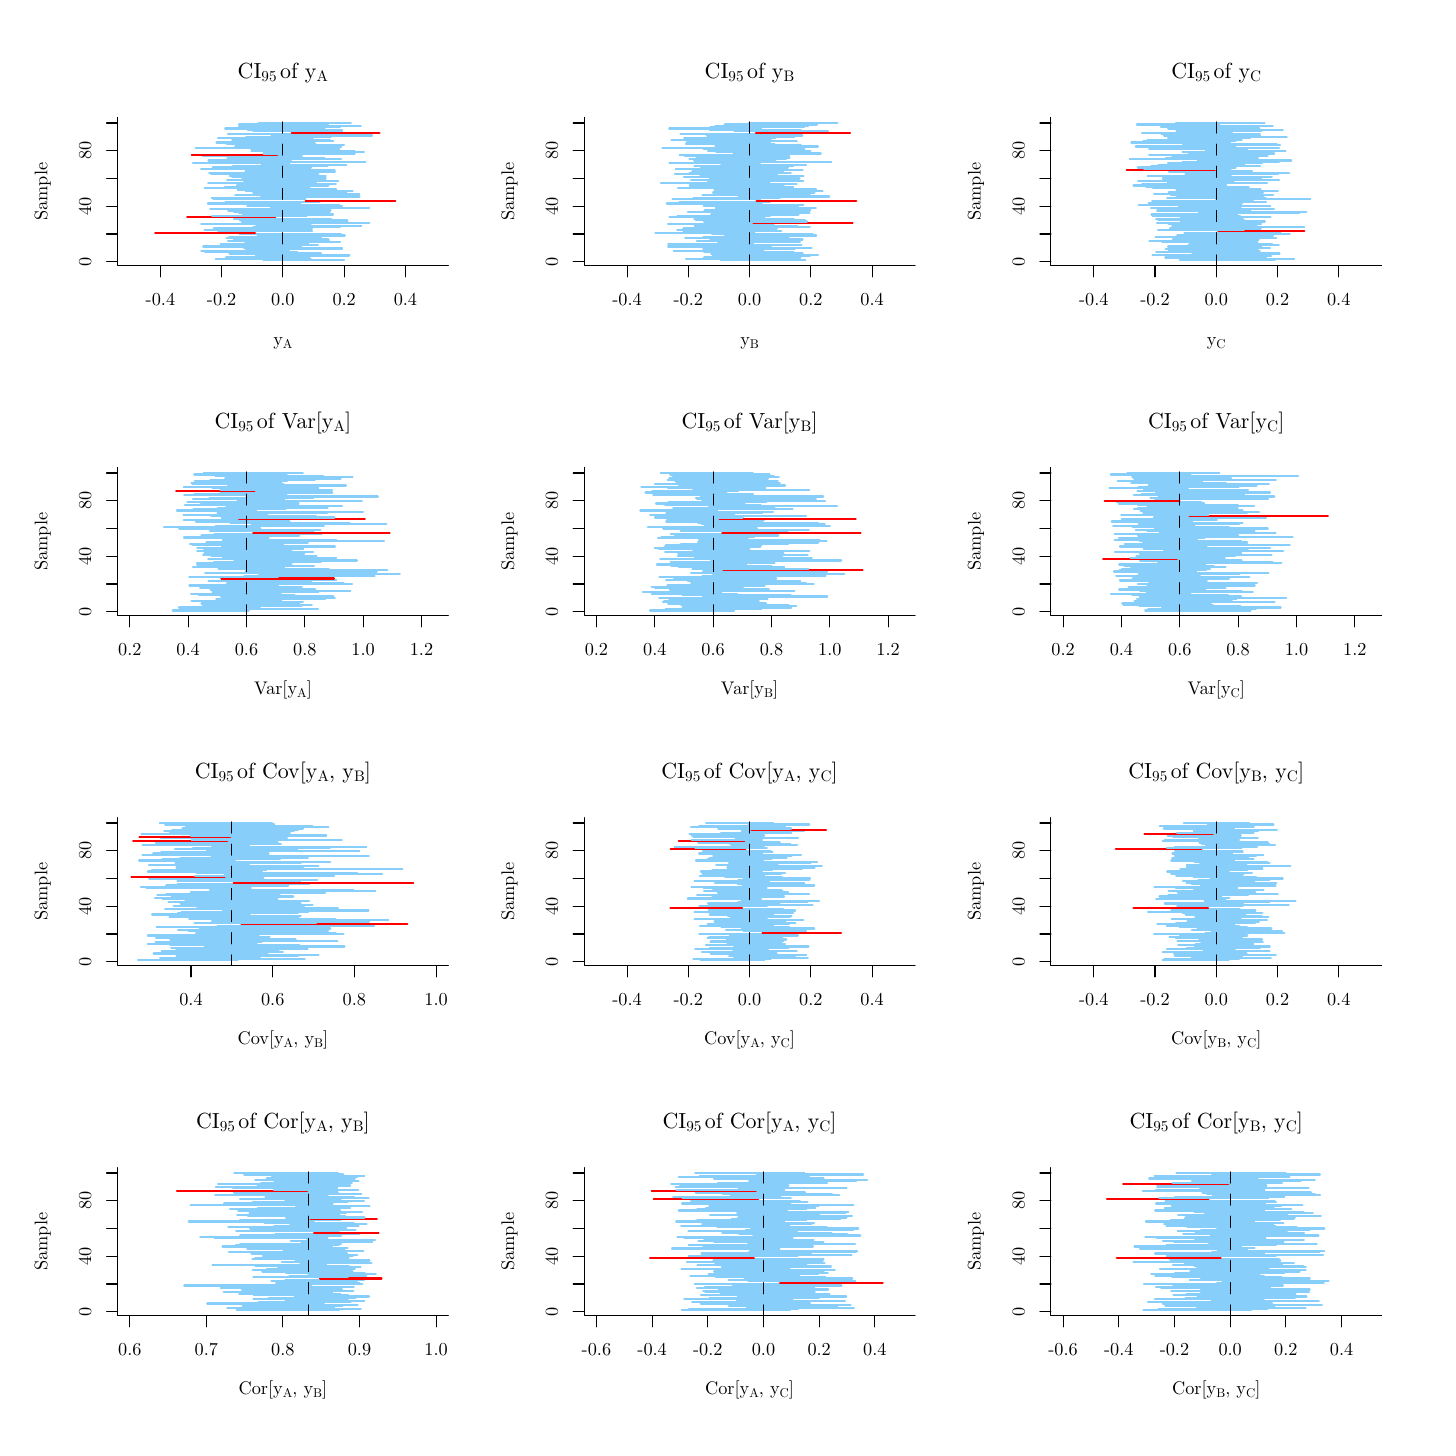
\begin{tikzpicture}[x=1pt,y=1pt]
\definecolor{fillColor}{RGB}{255,255,255}
\path[use as bounding box,fill=fillColor,fill opacity=0.00] (0,0) rectangle (505.89,505.89);
\begin{scope}
\path[clip] ( 32.47,419.81) rectangle (152.00,473.42);
\definecolor{drawColor}{RGB}{0,0,0}

\path[draw=drawColor,line width= 0.4pt,line join=round,line cap=round] (202.91,416.28) circle (  1.49);
\end{scope}
\begin{scope}
\path[clip] (  0.00,  0.00) rectangle (505.89,505.89);
\definecolor{drawColor}{RGB}{0,0,0}

\path[draw=drawColor,line width= 0.4pt,line join=round,line cap=round] ( 47.97,419.81) -- (136.50,419.81);

\path[draw=drawColor,line width= 0.4pt,line join=round,line cap=round] ( 47.97,419.81) -- ( 47.97,415.85);

\path[draw=drawColor,line width= 0.4pt,line join=round,line cap=round] ( 70.10,419.81) -- ( 70.10,415.85);

\path[draw=drawColor,line width= 0.4pt,line join=round,line cap=round] ( 92.23,419.81) -- ( 92.23,415.85);

\path[draw=drawColor,line width= 0.4pt,line join=round,line cap=round] (114.37,419.81) -- (114.37,415.85);

\path[draw=drawColor,line width= 0.4pt,line join=round,line cap=round] (136.50,419.81) -- (136.50,415.85);

\node[text=drawColor,anchor=base,inner sep=0pt, outer sep=0pt, scale=  0.66] at ( 47.97,405.55) {-0.4};

\node[text=drawColor,anchor=base,inner sep=0pt, outer sep=0pt, scale=  0.66] at ( 70.10,405.55) {-0.2};

\node[text=drawColor,anchor=base,inner sep=0pt, outer sep=0pt, scale=  0.66] at ( 92.23,405.55) {0.0};

\node[text=drawColor,anchor=base,inner sep=0pt, outer sep=0pt, scale=  0.66] at (114.37,405.55) {0.2};

\node[text=drawColor,anchor=base,inner sep=0pt, outer sep=0pt, scale=  0.66] at (136.50,405.55) {0.4};

\path[draw=drawColor,line width= 0.4pt,line join=round,line cap=round] ( 32.47,421.29) -- ( 32.47,471.43);

\path[draw=drawColor,line width= 0.4pt,line join=round,line cap=round] ( 32.47,421.29) -- ( 28.51,421.29);

\path[draw=drawColor,line width= 0.4pt,line join=round,line cap=round] ( 32.47,431.32) -- ( 28.51,431.32);

\path[draw=drawColor,line width= 0.4pt,line join=round,line cap=round] ( 32.47,441.35) -- ( 28.51,441.35);

\path[draw=drawColor,line width= 0.4pt,line join=round,line cap=round] ( 32.47,451.38) -- ( 28.51,451.38);

\path[draw=drawColor,line width= 0.4pt,line join=round,line cap=round] ( 32.47,461.40) -- ( 28.51,461.40);

\path[draw=drawColor,line width= 0.4pt,line join=round,line cap=round] ( 32.47,471.43) -- ( 28.51,471.43);

\node[text=drawColor,rotate= 90.00,anchor=base,inner sep=0pt, outer sep=0pt, scale=  0.66] at ( 22.97,421.29) {0};

\node[text=drawColor,rotate= 90.00,anchor=base,inner sep=0pt, outer sep=0pt, scale=  0.66] at ( 22.97,441.35) {40};

\node[text=drawColor,rotate= 90.00,anchor=base,inner sep=0pt, outer sep=0pt, scale=  0.66] at ( 22.97,461.40) {80};

\path[draw=drawColor,line width= 0.4pt,line join=round,line cap=round] ( 32.47,473.42) --
	( 32.47,419.81) --
	(152.00,419.81);
\end{scope}
\begin{scope}
\path[clip] (  0.00,379.42) rectangle (168.63,505.89);
\definecolor{drawColor}{RGB}{0,0,0}

\node[text=drawColor,anchor=base west,inner sep=0pt, outer sep=0pt, scale=  0.79] at ( 75.90,487.67) {CI};

\node[text=drawColor,anchor=base west,inner sep=0pt, outer sep=0pt, scale=  0.55] at ( 84.48,486.48) {95};

\node[text=drawColor,anchor=base west,inner sep=0pt, outer sep=0pt, scale=  0.79] at ( 90.02,487.67) {\hspace{1.5pt}of y};

\node[text=drawColor,anchor=base west,inner sep=0pt, outer sep=0pt, scale=  0.55] at (104.41,486.48) {A};

\node[text=drawColor,anchor=base west,inner sep=0pt, outer sep=0pt, scale=  0.66] at ( 88.76,391.00) {y};

\node[text=drawColor,anchor=base west,inner sep=0pt, outer sep=0pt, scale=  0.46] at ( 92.24,390.00) {A};

\node[text=drawColor,rotate= 90.00,anchor=base,inner sep=0pt, outer sep=0pt, scale=  0.66] at (  7.13,446.61) {Sample};
\end{scope}
\begin{scope}
\path[clip] ( 32.47,419.81) rectangle (152.00,473.42);
\definecolor{drawColor}{RGB}{135,206,250}

\path[draw=drawColor,line width= 0.8pt,line join=round,line cap=round] ( 85.22,421.80) --
	(114.33,421.80);

\path[draw=drawColor,line width= 0.8pt,line join=round,line cap=round] ( 67.93,422.30) --
	(102.27,422.30);

\path[draw=drawColor,line width= 0.8pt,line join=round,line cap=round] ( 71.71,422.80) --
	(101.71,422.80);

\path[draw=drawColor,line width= 0.8pt,line join=round,line cap=round] ( 82.85,423.30) --
	(116.01,423.30);

\path[draw=drawColor,line width= 0.8pt,line join=round,line cap=round] ( 82.39,423.80) --
	(116.29,423.80);

\path[draw=drawColor,line width= 0.8pt,line join=round,line cap=round] ( 72.95,424.30) --
	(105.95,424.30);

\path[draw=drawColor,line width= 0.8pt,line join=round,line cap=round] ( 64.13,424.80) --
	( 97.40,424.80);

\path[draw=drawColor,line width= 0.8pt,line join=round,line cap=round] ( 62.74,425.30) --
	( 94.44,425.30);

\path[draw=drawColor,line width= 0.8pt,line join=round,line cap=round] ( 78.81,425.81) --
	(113.63,425.81);

\path[draw=drawColor,line width= 0.8pt,line join=round,line cap=round] ( 78.10,426.31) --
	(113.59,426.31);

\path[draw=drawColor,line width= 0.8pt,line join=round,line cap=round] ( 63.42,426.81) --
	( 98.81,426.81);

\path[draw=drawColor,line width= 0.8pt,line join=round,line cap=round] ( 72.24,427.31) --
	(104.89,427.31);

\path[draw=drawColor,line width= 0.8pt,line join=round,line cap=round] ( 69.76,427.81) --
	(101.40,427.81);

\path[draw=drawColor,line width= 0.8pt,line join=round,line cap=round] ( 78.57,428.31) --
	(112.93,428.31);

\path[draw=drawColor,line width= 0.8pt,line join=round,line cap=round] ( 72.38,428.81) --
	(108.90,428.81);

\path[draw=drawColor,line width= 0.8pt,line join=round,line cap=round] ( 74.59,429.32) --
	(108.72,429.32);

\path[draw=drawColor,line width= 0.8pt,line join=round,line cap=round] ( 71.86,429.82) --
	(104.67,429.82);

\path[draw=drawColor,line width= 0.8pt,line join=round,line cap=round] ( 72.86,430.32) --
	(106.05,430.32);

\path[draw=drawColor,line width= 0.8pt,line join=round,line cap=round] ( 83.14,430.82) --
	(114.56,430.82);

\path[draw=drawColor,line width= 0.8pt,line join=round,line cap=round] ( 76.55,431.32) --
	(113.19,431.32);
\definecolor{drawColor}{RGB}{255,0,0}

\path[draw=drawColor,line width= 0.8pt,line join=round,line cap=round] ( 46.07,431.82) --
	( 82.13,431.82);
\definecolor{drawColor}{RGB}{135,206,250}

\path[draw=drawColor,line width= 0.8pt,line join=round,line cap=round] ( 68.86,432.32) --
	(102.74,432.32);

\path[draw=drawColor,line width= 0.8pt,line join=round,line cap=round] ( 63.98,432.83) --
	( 99.57,432.83);

\path[draw=drawColor,line width= 0.8pt,line join=round,line cap=round] ( 67.29,433.33) --
	(102.71,433.33);

\path[draw=drawColor,line width= 0.8pt,line join=round,line cap=round] ( 81.47,433.83) --
	(112.88,433.83);

\path[draw=drawColor,line width= 0.8pt,line join=round,line cap=round] ( 82.52,434.33) --
	(120.59,434.33);

\path[draw=drawColor,line width= 0.8pt,line join=round,line cap=round] ( 62.69,434.83) --
	(102.31,434.83);

\path[draw=drawColor,line width= 0.8pt,line join=round,line cap=round] ( 90.01,435.33) --
	(123.47,435.33);

\path[draw=drawColor,line width= 0.8pt,line join=round,line cap=round] ( 77.31,435.83) --
	(115.51,435.83);

\path[draw=drawColor,line width= 0.8pt,line join=round,line cap=round] ( 76.61,436.34) --
	(115.47,436.34);

\path[draw=drawColor,line width= 0.8pt,line join=round,line cap=round] ( 74.53,436.84) --
	(109.60,436.84);
\definecolor{drawColor}{RGB}{255,0,0}

\path[draw=drawColor,line width= 0.8pt,line join=round,line cap=round] ( 57.61,437.34) --
	( 89.50,437.34);
\definecolor{drawColor}{RGB}{135,206,250}

\path[draw=drawColor,line width= 0.8pt,line join=round,line cap=round] ( 66.70,437.84) --
	(100.77,437.84);

\path[draw=drawColor,line width= 0.8pt,line join=round,line cap=round] ( 77.87,438.34) --
	(110.31,438.34);

\path[draw=drawColor,line width= 0.8pt,line join=round,line cap=round] ( 76.43,438.84) --
	(108.83,438.84);

\path[draw=drawColor,line width= 0.8pt,line join=round,line cap=round] ( 74.54,439.34) --
	(109.07,439.34);

\path[draw=drawColor,line width= 0.8pt,line join=round,line cap=round] ( 72.50,439.85) --
	(109.45,439.85);

\path[draw=drawColor,line width= 0.8pt,line join=round,line cap=round] ( 65.98,440.35) --
	( 99.81,440.35);

\path[draw=drawColor,line width= 0.8pt,line join=round,line cap=round] ( 87.84,440.85) --
	(123.42,440.85);

\path[draw=drawColor,line width= 0.8pt,line join=round,line cap=round] ( 79.38,441.35) --
	(113.61,441.35);

\path[draw=drawColor,line width= 0.8pt,line join=round,line cap=round] ( 79.45,441.85) --
	(112.65,441.85);

\path[draw=drawColor,line width= 0.8pt,line join=round,line cap=round] ( 65.13,442.35) --
	( 98.49,442.35);

\path[draw=drawColor,line width= 0.8pt,line join=round,line cap=round] ( 71.49,442.85) --
	(105.48,442.85);
\definecolor{drawColor}{RGB}{255,0,0}

\path[draw=drawColor,line width= 0.8pt,line join=round,line cap=round] (100.43,443.35) --
	(132.87,443.35);
\definecolor{drawColor}{RGB}{135,206,250}

\path[draw=drawColor,line width= 0.8pt,line join=round,line cap=round] ( 67.09,443.86) --
	(100.38,443.86);

\path[draw=drawColor,line width= 0.8pt,line join=round,line cap=round] ( 66.51,444.36) --
	( 98.97,444.36);

\path[draw=drawColor,line width= 0.8pt,line join=round,line cap=round] ( 84.41,444.86) --
	(119.91,444.86);

\path[draw=drawColor,line width= 0.8pt,line join=round,line cap=round] ( 74.97,445.36) --
	(106.81,445.36);

\path[draw=drawColor,line width= 0.8pt,line join=round,line cap=round] ( 88.36,445.86) --
	(119.86,445.86);

\path[draw=drawColor,line width= 0.8pt,line join=round,line cap=round] ( 81.50,446.36) --
	(115.11,446.36);

\path[draw=drawColor,line width= 0.8pt,line join=round,line cap=round] ( 78.75,446.86) --
	(117.40,446.86);

\path[draw=drawColor,line width= 0.8pt,line join=round,line cap=round] ( 75.86,447.37) --
	(111.44,447.37);

\path[draw=drawColor,line width= 0.8pt,line join=round,line cap=round] ( 63.98,447.87) --
	( 94.68,447.87);

\path[draw=drawColor,line width= 0.8pt,line join=round,line cap=round] ( 71.29,448.37) --
	(102.00,448.37);

\path[draw=drawColor,line width= 0.8pt,line join=round,line cap=round] ( 75.64,448.87) --
	(108.63,448.87);

\path[draw=drawColor,line width= 0.8pt,line join=round,line cap=round] ( 76.76,449.37) --
	(111.35,449.37);

\path[draw=drawColor,line width= 0.8pt,line join=round,line cap=round] ( 65.20,449.87) --
	(104.21,449.87);

\path[draw=drawColor,line width= 0.8pt,line join=round,line cap=round] ( 78.17,450.37) --
	(112.20,450.37);

\path[draw=drawColor,line width= 0.8pt,line join=round,line cap=round] ( 72.10,450.88) --
	(106.60,450.88);

\path[draw=drawColor,line width= 0.8pt,line join=round,line cap=round] ( 77.61,451.38) --
	(107.66,451.38);

\path[draw=drawColor,line width= 0.8pt,line join=round,line cap=round] ( 73.90,451.88) --
	(101.71,451.88);

\path[draw=drawColor,line width= 0.8pt,line join=round,line cap=round] ( 73.01,452.38) --
	(107.74,452.38);

\path[draw=drawColor,line width= 0.8pt,line join=round,line cap=round] ( 66.27,452.88) --
	(105.07,452.88);

\path[draw=drawColor,line width= 0.8pt,line join=round,line cap=round] ( 65.61,453.38) --
	(102.08,453.38);

\path[draw=drawColor,line width= 0.8pt,line join=round,line cap=round] ( 78.70,453.88) --
	(110.99,453.88);

\path[draw=drawColor,line width= 0.8pt,line join=round,line cap=round] ( 80.22,454.39) --
	(110.86,454.39);

\path[draw=drawColor,line width= 0.8pt,line join=round,line cap=round] ( 62.65,454.89) --
	(100.10,454.89);

\path[draw=drawColor,line width= 0.8pt,line join=round,line cap=round] ( 66.89,455.39) --
	(102.34,455.39);

\path[draw=drawColor,line width= 0.8pt,line join=round,line cap=round] ( 74.15,455.89) --
	(108.35,455.89);

\path[draw=drawColor,line width= 0.8pt,line join=round,line cap=round] ( 84.49,456.39) --
	(115.11,456.39);

\path[draw=drawColor,line width= 0.8pt,line join=round,line cap=round] ( 59.73,456.89) --
	( 94.68,456.89);

\path[draw=drawColor,line width= 0.8pt,line join=round,line cap=round] ( 84.69,457.39) --
	(122.03,457.39);

\path[draw=drawColor,line width= 0.8pt,line join=round,line cap=round] ( 65.33,457.89) --
	( 95.04,457.89);

\path[draw=drawColor,line width= 0.8pt,line join=round,line cap=round] ( 81.25,458.40) --
	(113.22,458.40);

\path[draw=drawColor,line width= 0.8pt,line join=round,line cap=round] ( 72.18,458.90) --
	(107.19,458.90);

\path[draw=drawColor,line width= 0.8pt,line join=round,line cap=round] ( 63.13,459.40) --
	( 99.11,459.40);
\definecolor{drawColor}{RGB}{255,0,0}

\path[draw=drawColor,line width= 0.8pt,line join=round,line cap=round] ( 59.26,459.90) --
	( 90.08,459.90);
\definecolor{drawColor}{RGB}{135,206,250}

\path[draw=drawColor,line width= 0.8pt,line join=round,line cap=round] ( 85.19,460.40) --
	(118.15,460.40);

\path[draw=drawColor,line width= 0.8pt,line join=round,line cap=round] ( 90.38,460.90) --
	(121.53,460.90);

\path[draw=drawColor,line width= 0.8pt,line join=round,line cap=round] ( 80.85,461.40) --
	(118.12,461.40);

\path[draw=drawColor,line width= 0.8pt,line join=round,line cap=round] ( 80.74,461.91) --
	(112.64,461.91);

\path[draw=drawColor,line width= 0.8pt,line join=round,line cap=round] ( 60.68,462.41) --
	( 94.68,462.41);

\path[draw=drawColor,line width= 0.8pt,line join=round,line cap=round] ( 74.99,462.91) --
	(113.26,462.91);

\path[draw=drawColor,line width= 0.8pt,line join=round,line cap=round] ( 83.63,463.41) --
	(114.35,463.41);

\path[draw=drawColor,line width= 0.8pt,line join=round,line cap=round] ( 71.96,463.91) --
	(104.04,463.91);

\path[draw=drawColor,line width= 0.8pt,line join=round,line cap=round] ( 68.23,464.41) --
	(103.54,464.41);

\path[draw=drawColor,line width= 0.8pt,line join=round,line cap=round] ( 80.83,464.91) --
	(110.43,464.91);

\path[draw=drawColor,line width= 0.8pt,line join=round,line cap=round] ( 73.87,465.42) --
	(109.17,465.42);

\path[draw=drawColor,line width= 0.8pt,line join=round,line cap=round] ( 68.77,465.92) --
	(103.13,465.92);

\path[draw=drawColor,line width= 0.8pt,line join=round,line cap=round] ( 78.92,466.42) --
	(109.56,466.42);

\path[draw=drawColor,line width= 0.8pt,line join=round,line cap=round] ( 88.21,466.92) --
	(124.43,466.92);

\path[draw=drawColor,line width= 0.8pt,line join=round,line cap=round] ( 72.32,467.42) --
	(104.15,467.42);
\definecolor{drawColor}{RGB}{255,0,0}

\path[draw=drawColor,line width= 0.8pt,line join=round,line cap=round] ( 95.43,467.92) --
	(127.12,467.92);
\definecolor{drawColor}{RGB}{135,206,250}

\path[draw=drawColor,line width= 0.8pt,line join=round,line cap=round] ( 81.48,468.42) --
	(113.59,468.42);

\path[draw=drawColor,line width= 0.8pt,line join=round,line cap=round] ( 79.54,468.93) --
	(113.64,468.93);

\path[draw=drawColor,line width= 0.8pt,line join=round,line cap=round] ( 71.37,469.43) --
	(107.25,469.43);

\path[draw=drawColor,line width= 0.8pt,line join=round,line cap=round] ( 76.21,469.93) --
	(112.87,469.93);

\path[draw=drawColor,line width= 0.8pt,line join=round,line cap=round] ( 85.69,470.43) --
	(120.39,470.43);

\path[draw=drawColor,line width= 0.8pt,line join=round,line cap=round] ( 76.35,470.93) --
	(108.42,470.93);

\path[draw=drawColor,line width= 0.8pt,line join=round,line cap=round] ( 83.52,471.43) --
	(116.79,471.43);
\definecolor{drawColor}{RGB}{0,0,0}

\path[draw=drawColor,line width= 0.4pt,dash pattern=on 4pt off 4pt ,line join=round,line cap=round] ( 92.23,419.81) -- ( 92.23,473.42);
\end{scope}
\begin{scope}
\path[clip] (201.10,419.81) rectangle (320.63,473.42);
\definecolor{drawColor}{RGB}{0,0,0}

\path[draw=drawColor,line width= 0.4pt,line join=round,line cap=round] (371.54,416.28) circle (  1.49);
\end{scope}
\begin{scope}
\path[clip] (  0.00,  0.00) rectangle (505.89,505.89);
\definecolor{drawColor}{RGB}{0,0,0}

\path[draw=drawColor,line width= 0.4pt,line join=round,line cap=round] (216.60,419.81) -- (305.13,419.81);

\path[draw=drawColor,line width= 0.4pt,line join=round,line cap=round] (216.60,419.81) -- (216.60,415.85);

\path[draw=drawColor,line width= 0.4pt,line join=round,line cap=round] (238.73,419.81) -- (238.73,415.85);

\path[draw=drawColor,line width= 0.4pt,line join=round,line cap=round] (260.87,419.81) -- (260.87,415.85);

\path[draw=drawColor,line width= 0.4pt,line join=round,line cap=round] (283.00,419.81) -- (283.00,415.85);

\path[draw=drawColor,line width= 0.4pt,line join=round,line cap=round] (305.13,419.81) -- (305.13,415.85);

\node[text=drawColor,anchor=base,inner sep=0pt, outer sep=0pt, scale=  0.66] at (216.60,405.55) {-0.4};

\node[text=drawColor,anchor=base,inner sep=0pt, outer sep=0pt, scale=  0.66] at (238.73,405.55) {-0.2};

\node[text=drawColor,anchor=base,inner sep=0pt, outer sep=0pt, scale=  0.66] at (260.87,405.55) {0.0};

\node[text=drawColor,anchor=base,inner sep=0pt, outer sep=0pt, scale=  0.66] at (283.00,405.55) {0.2};

\node[text=drawColor,anchor=base,inner sep=0pt, outer sep=0pt, scale=  0.66] at (305.13,405.55) {0.4};

\path[draw=drawColor,line width= 0.4pt,line join=round,line cap=round] (201.10,421.29) -- (201.10,471.43);

\path[draw=drawColor,line width= 0.4pt,line join=round,line cap=round] (201.10,421.29) -- (197.14,421.29);

\path[draw=drawColor,line width= 0.4pt,line join=round,line cap=round] (201.10,431.32) -- (197.14,431.32);

\path[draw=drawColor,line width= 0.4pt,line join=round,line cap=round] (201.10,441.35) -- (197.14,441.35);

\path[draw=drawColor,line width= 0.4pt,line join=round,line cap=round] (201.10,451.38) -- (197.14,451.38);

\path[draw=drawColor,line width= 0.4pt,line join=round,line cap=round] (201.10,461.40) -- (197.14,461.40);

\path[draw=drawColor,line width= 0.4pt,line join=round,line cap=round] (201.10,471.43) -- (197.14,471.43);

\node[text=drawColor,rotate= 90.00,anchor=base,inner sep=0pt, outer sep=0pt, scale=  0.66] at (191.60,421.29) {0};

\node[text=drawColor,rotate= 90.00,anchor=base,inner sep=0pt, outer sep=0pt, scale=  0.66] at (191.60,441.35) {40};

\node[text=drawColor,rotate= 90.00,anchor=base,inner sep=0pt, outer sep=0pt, scale=  0.66] at (191.60,461.40) {80};

\path[draw=drawColor,line width= 0.4pt,line join=round,line cap=round] (201.10,473.42) --
	(201.10,419.81) --
	(320.63,419.81);
\end{scope}
\begin{scope}
\path[clip] (168.63,379.42) rectangle (337.26,505.89);
\definecolor{drawColor}{RGB}{0,0,0}

\node[text=drawColor,anchor=base west,inner sep=0pt, outer sep=0pt, scale=  0.79] at (244.65,487.67) {CI};

\node[text=drawColor,anchor=base west,inner sep=0pt, outer sep=0pt, scale=  0.55] at (253.23,486.48) {95};

\node[text=drawColor,anchor=base west,inner sep=0pt, outer sep=0pt, scale=  0.79] at (258.77,487.67) {\hspace{1.5pt}of y};

\node[text=drawColor,anchor=base west,inner sep=0pt, outer sep=0pt, scale=  0.55] at (273.15,486.48) {B};

\node[text=drawColor,anchor=base west,inner sep=0pt, outer sep=0pt, scale=  0.66] at (257.49,391.00) {y};

\node[text=drawColor,anchor=base west,inner sep=0pt, outer sep=0pt, scale=  0.46] at (260.97,390.00) {B};

\node[text=drawColor,rotate= 90.00,anchor=base,inner sep=0pt, outer sep=0pt, scale=  0.66] at (175.76,446.61) {Sample};
\end{scope}
\begin{scope}
\path[clip] (201.10,419.81) rectangle (320.63,473.42);
\definecolor{drawColor}{RGB}{135,206,250}

\path[draw=drawColor,line width= 0.8pt,line join=round,line cap=round] (250.39,421.80) --
	(280.99,421.80);

\path[draw=drawColor,line width= 0.8pt,line join=round,line cap=round] (237.85,422.30) --
	(270.53,422.30);

\path[draw=drawColor,line width= 0.8pt,line join=round,line cap=round] (244.42,422.80) --
	(279.21,422.80);

\path[draw=drawColor,line width= 0.8pt,line join=round,line cap=round] (247.50,423.30) --
	(282.64,423.30);

\path[draw=drawColor,line width= 0.8pt,line join=round,line cap=round] (251.04,423.80) --
	(285.64,423.80);

\path[draw=drawColor,line width= 0.8pt,line join=round,line cap=round] (247.00,424.30) --
	(280.01,424.30);

\path[draw=drawColor,line width= 0.8pt,line join=round,line cap=round] (244.48,424.80) --
	(276.78,424.80);

\path[draw=drawColor,line width= 0.8pt,line join=round,line cap=round] (233.43,425.30) --
	(265.91,425.30);

\path[draw=drawColor,line width= 0.8pt,line join=round,line cap=round] (244.11,425.81) --
	(277.23,425.81);

\path[draw=drawColor,line width= 0.8pt,line join=round,line cap=round] (251.43,426.31) --
	(283.25,426.31);

\path[draw=drawColor,line width= 0.8pt,line join=round,line cap=round] (231.44,426.81) --
	(268.63,426.81);

\path[draw=drawColor,line width= 0.8pt,line join=round,line cap=round] (244.88,427.31) --
	(279.62,427.31);

\path[draw=drawColor,line width= 0.8pt,line join=round,line cap=round] (231.41,427.81) --
	(262.24,427.81);

\path[draw=drawColor,line width= 0.8pt,line join=round,line cap=round] (249.44,428.31) --
	(279.06,428.31);

\path[draw=drawColor,line width= 0.8pt,line join=round,line cap=round] (241.78,428.81) --
	(276.79,428.81);

\path[draw=drawColor,line width= 0.8pt,line join=round,line cap=round] (246.77,429.32) --
	(279.99,429.32);

\path[draw=drawColor,line width= 0.8pt,line join=round,line cap=round] (237.59,429.82) --
	(268.90,429.82);

\path[draw=drawColor,line width= 0.8pt,line join=round,line cap=round] (244.21,430.32) --
	(275.03,430.32);

\path[draw=drawColor,line width= 0.8pt,line join=round,line cap=round] (252.01,430.82) --
	(284.91,430.82);

\path[draw=drawColor,line width= 0.8pt,line join=round,line cap=round] (247.32,431.32) --
	(283.62,431.32);

\path[draw=drawColor,line width= 0.8pt,line join=round,line cap=round] (226.86,431.82) --
	(262.63,431.82);

\path[draw=drawColor,line width= 0.8pt,line join=round,line cap=round] (236.94,432.32) --
	(272.34,432.32);

\path[draw=drawColor,line width= 0.8pt,line join=round,line cap=round] (234.73,432.83) --
	(267.46,432.83);

\path[draw=drawColor,line width= 0.8pt,line join=round,line cap=round] (236.94,433.33) --
	(270.68,433.33);

\path[draw=drawColor,line width= 0.8pt,line join=round,line cap=round] (250.73,433.83) --
	(282.60,433.83);

\path[draw=drawColor,line width= 0.8pt,line join=round,line cap=round] (241.02,434.33) --
	(278.09,434.33);

\path[draw=drawColor,line width= 0.8pt,line join=round,line cap=round] (231.35,434.83) --
	(269.61,434.83);
\definecolor{drawColor}{RGB}{255,0,0}

\path[draw=drawColor,line width= 0.8pt,line join=round,line cap=round] (262.27,435.33) --
	(298.05,435.33);
\definecolor{drawColor}{RGB}{135,206,250}

\path[draw=drawColor,line width= 0.8pt,line join=round,line cap=round] (244.41,435.83) --
	(281.57,435.83);

\path[draw=drawColor,line width= 0.8pt,line join=round,line cap=round] (241.43,436.34) --
	(280.82,436.34);

\path[draw=drawColor,line width= 0.8pt,line join=round,line cap=round] (240.87,436.84) --
	(276.82,436.84);

\path[draw=drawColor,line width= 0.8pt,line join=round,line cap=round] (231.93,437.34) --
	(266.24,437.34);

\path[draw=drawColor,line width= 0.8pt,line join=round,line cap=round] (234.76,437.84) --
	(268.15,437.84);

\path[draw=drawColor,line width= 0.8pt,line join=round,line cap=round] (247.00,438.34) --
	(278.54,438.34);

\path[draw=drawColor,line width= 0.8pt,line join=round,line cap=round] (248.91,438.84) --
	(282.52,438.84);

\path[draw=drawColor,line width= 0.8pt,line join=round,line cap=round] (238.55,439.34) --
	(271.84,439.34);

\path[draw=drawColor,line width= 0.8pt,line join=round,line cap=round] (244.57,439.85) --
	(282.63,439.85);

\path[draw=drawColor,line width= 0.8pt,line join=round,line cap=round] (250.91,440.35) --
	(282.88,440.35);

\path[draw=drawColor,line width= 0.8pt,line join=round,line cap=round] (248.62,440.85) --
	(284.79,440.85);

\path[draw=drawColor,line width= 0.8pt,line join=round,line cap=round] (244.27,441.35) --
	(278.44,441.35);

\path[draw=drawColor,line width= 0.8pt,line join=round,line cap=round] (244.42,441.85) --
	(280.31,441.85);

\path[draw=drawColor,line width= 0.8pt,line join=round,line cap=round] (230.96,442.35) --
	(265.21,442.35);

\path[draw=drawColor,line width= 0.8pt,line join=round,line cap=round] (235.53,442.85) --
	(268.13,442.85);
\definecolor{drawColor}{RGB}{255,0,0}

\path[draw=drawColor,line width= 0.8pt,line join=round,line cap=round] (263.38,443.35) --
	(299.39,443.35);
\definecolor{drawColor}{RGB}{135,206,250}

\path[draw=drawColor,line width= 0.8pt,line join=round,line cap=round] (232.98,443.86) --
	(264.76,443.86);

\path[draw=drawColor,line width= 0.8pt,line join=round,line cap=round] (240.59,444.36) --
	(271.81,444.36);

\path[draw=drawColor,line width= 0.8pt,line join=round,line cap=round] (257.03,444.86) --
	(289.62,444.86);

\path[draw=drawColor,line width= 0.8pt,line join=round,line cap=round] (243.79,445.36) --
	(276.48,445.36);

\path[draw=drawColor,line width= 0.8pt,line join=round,line cap=round] (248.10,445.86) --
	(282.68,445.86);

\path[draw=drawColor,line width= 0.8pt,line join=round,line cap=round] (247.67,446.36) --
	(284.26,446.36);

\path[draw=drawColor,line width= 0.8pt,line join=round,line cap=round] (250.13,446.86) --
	(287.27,446.86);

\path[draw=drawColor,line width= 0.8pt,line join=round,line cap=round] (248.17,447.37) --
	(284.85,447.37);

\path[draw=drawColor,line width= 0.8pt,line join=round,line cap=round] (234.95,447.87) --
	(266.62,447.87);

\path[draw=drawColor,line width= 0.8pt,line join=round,line cap=round] (244.51,448.37) --
	(276.64,448.37);

\path[draw=drawColor,line width= 0.8pt,line join=round,line cap=round] (239.24,448.87) --
	(273.12,448.87);

\path[draw=drawColor,line width= 0.8pt,line join=round,line cap=round] (244.49,449.37) --
	(277.81,449.37);

\path[draw=drawColor,line width= 0.8pt,line join=round,line cap=round] (228.85,449.87) --
	(268.11,449.87);

\path[draw=drawColor,line width= 0.8pt,line join=round,line cap=round] (245.75,450.37) --
	(280.29,450.37);

\path[draw=drawColor,line width= 0.8pt,line join=round,line cap=round] (239.65,450.88) --
	(275.63,450.88);

\path[draw=drawColor,line width= 0.8pt,line join=round,line cap=round] (246.52,451.38) --
	(278.87,451.38);

\path[draw=drawColor,line width= 0.8pt,line join=round,line cap=round] (237.09,451.88) --
	(267.38,451.88);

\path[draw=drawColor,line width= 0.8pt,line join=round,line cap=round] (243.02,452.38) --
	(280.37,452.38);

\path[draw=drawColor,line width= 0.8pt,line join=round,line cap=round] (233.85,452.88) --
	(270.87,452.88);

\path[draw=drawColor,line width= 0.8pt,line join=round,line cap=round] (239.14,453.38) --
	(275.74,453.38);

\path[draw=drawColor,line width= 0.8pt,line join=round,line cap=round] (240.16,453.88) --
	(272.91,453.88);

\path[draw=drawColor,line width= 0.8pt,line join=round,line cap=round] (247.11,454.39) --
	(279.99,454.39);

\path[draw=drawColor,line width= 0.8pt,line join=round,line cap=round] (234.16,454.89) --
	(273.12,454.89);

\path[draw=drawColor,line width= 0.8pt,line join=round,line cap=round] (243.42,455.39) --
	(274.69,455.39);

\path[draw=drawColor,line width= 0.8pt,line join=round,line cap=round] (240.91,455.89) --
	(276.71,455.89);

\path[draw=drawColor,line width= 0.8pt,line join=round,line cap=round] (250.60,456.39) --
	(281.24,456.39);

\path[draw=drawColor,line width= 0.8pt,line join=round,line cap=round] (231.89,456.89) --
	(264.62,456.89);

\path[draw=drawColor,line width= 0.8pt,line join=round,line cap=round] (256.88,457.39) --
	(290.39,457.39);

\path[draw=drawColor,line width= 0.8pt,line join=round,line cap=round] (240.87,457.89) --
	(270.12,457.89);

\path[draw=drawColor,line width= 0.8pt,line join=round,line cap=round] (239.13,458.40) --
	(274.01,458.40);

\path[draw=drawColor,line width= 0.8pt,line join=round,line cap=round] (241.67,458.90) --
	(275.29,458.90);

\path[draw=drawColor,line width= 0.8pt,line join=round,line cap=round] (237.42,459.40) --
	(275.23,459.40);

\path[draw=drawColor,line width= 0.8pt,line join=round,line cap=round] (235.57,459.90) --
	(268.20,459.90);

\path[draw=drawColor,line width= 0.8pt,line join=round,line cap=round] (255.15,460.40) --
	(286.56,460.40);

\path[draw=drawColor,line width= 0.8pt,line join=round,line cap=round] (248.75,460.90) --
	(281.77,460.90);

\path[draw=drawColor,line width= 0.8pt,line join=round,line cap=round] (245.82,461.40) --
	(282.86,461.40);

\path[draw=drawColor,line width= 0.8pt,line join=round,line cap=round] (244.25,461.91) --
	(280.69,461.91);

\path[draw=drawColor,line width= 0.8pt,line join=round,line cap=round] (229.34,462.41) --
	(265.69,462.41);

\path[draw=drawColor,line width= 0.8pt,line join=round,line cap=round] (248.62,462.91) --
	(285.53,462.91);

\path[draw=drawColor,line width= 0.8pt,line join=round,line cap=round] (248.37,463.41) --
	(279.40,463.41);

\path[draw=drawColor,line width= 0.8pt,line join=round,line cap=round] (237.81,463.91) --
	(269.87,463.91);

\path[draw=drawColor,line width= 0.8pt,line join=round,line cap=round] (238.14,464.41) --
	(268.13,464.41);

\path[draw=drawColor,line width= 0.8pt,line join=round,line cap=round] (246.99,464.91) --
	(277.91,464.91);

\path[draw=drawColor,line width= 0.8pt,line join=round,line cap=round] (232.63,465.42) --
	(268.63,465.42);

\path[draw=drawColor,line width= 0.8pt,line join=round,line cap=round] (237.22,465.92) --
	(270.17,465.92);

\path[draw=drawColor,line width= 0.8pt,line join=round,line cap=round] (247.64,466.42) --
	(277.03,466.42);

\path[draw=drawColor,line width= 0.8pt,line join=round,line cap=round] (245.52,466.92) --
	(279.88,466.92);

\path[draw=drawColor,line width= 0.8pt,line join=round,line cap=round] (235.87,467.42) --
	(267.14,467.42);
\definecolor{drawColor}{RGB}{255,0,0}

\path[draw=drawColor,line width= 0.8pt,line join=round,line cap=round] (263.17,467.92) --
	(297.17,467.92);
\definecolor{drawColor}{RGB}{135,206,250}

\path[draw=drawColor,line width= 0.8pt,line join=round,line cap=round] (255.38,468.42) --
	(289.23,468.42);

\path[draw=drawColor,line width= 0.8pt,line join=round,line cap=round] (246.48,468.93) --
	(279.40,468.93);

\path[draw=drawColor,line width= 0.8pt,line join=round,line cap=round] (231.83,469.43) --
	(264.98,469.43);

\path[draw=drawColor,line width= 0.8pt,line join=round,line cap=round] (246.67,469.93) --
	(280.59,469.93);

\path[draw=drawColor,line width= 0.8pt,line join=round,line cap=round] (248.45,470.43) --
	(282.02,470.43);

\path[draw=drawColor,line width= 0.8pt,line join=round,line cap=round] (251.92,470.93) --
	(285.18,470.93);

\path[draw=drawColor,line width= 0.8pt,line join=round,line cap=round] (260.59,471.43) --
	(292.62,471.43);
\definecolor{drawColor}{RGB}{0,0,0}

\path[draw=drawColor,line width= 0.4pt,dash pattern=on 4pt off 4pt ,line join=round,line cap=round] (260.87,419.81) -- (260.87,473.42);
\end{scope}
\begin{scope}
\path[clip] (  0.00,  0.00) rectangle (505.89,505.89);
\definecolor{drawColor}{RGB}{0,0,0}

\path[draw=drawColor,line width= 0.4pt,line join=round,line cap=round] (385.23,419.81) -- (473.76,419.81);

\path[draw=drawColor,line width= 0.4pt,line join=round,line cap=round] (385.23,419.81) -- (385.23,415.85);

\path[draw=drawColor,line width= 0.4pt,line join=round,line cap=round] (407.36,419.81) -- (407.36,415.85);

\path[draw=drawColor,line width= 0.4pt,line join=round,line cap=round] (429.50,419.81) -- (429.50,415.85);

\path[draw=drawColor,line width= 0.4pt,line join=round,line cap=round] (451.63,419.81) -- (451.63,415.85);

\path[draw=drawColor,line width= 0.4pt,line join=round,line cap=round] (473.76,419.81) -- (473.76,415.85);

\node[text=drawColor,anchor=base,inner sep=0pt, outer sep=0pt, scale=  0.66] at (385.23,405.55) {-0.4};

\node[text=drawColor,anchor=base,inner sep=0pt, outer sep=0pt, scale=  0.66] at (407.36,405.55) {-0.2};

\node[text=drawColor,anchor=base,inner sep=0pt, outer sep=0pt, scale=  0.66] at (429.50,405.55) {0.0};

\node[text=drawColor,anchor=base,inner sep=0pt, outer sep=0pt, scale=  0.66] at (451.63,405.55) {0.2};

\node[text=drawColor,anchor=base,inner sep=0pt, outer sep=0pt, scale=  0.66] at (473.76,405.55) {0.4};

\path[draw=drawColor,line width= 0.4pt,line join=round,line cap=round] (369.73,421.29) -- (369.73,471.43);

\path[draw=drawColor,line width= 0.4pt,line join=round,line cap=round] (369.73,421.29) -- (365.77,421.29);

\path[draw=drawColor,line width= 0.4pt,line join=round,line cap=round] (369.73,431.32) -- (365.77,431.32);

\path[draw=drawColor,line width= 0.4pt,line join=round,line cap=round] (369.73,441.35) -- (365.77,441.35);

\path[draw=drawColor,line width= 0.4pt,line join=round,line cap=round] (369.73,451.38) -- (365.77,451.38);

\path[draw=drawColor,line width= 0.4pt,line join=round,line cap=round] (369.73,461.40) -- (365.77,461.40);

\path[draw=drawColor,line width= 0.4pt,line join=round,line cap=round] (369.73,471.43) -- (365.77,471.43);

\node[text=drawColor,rotate= 90.00,anchor=base,inner sep=0pt, outer sep=0pt, scale=  0.66] at (360.23,421.29) {0};

\node[text=drawColor,rotate= 90.00,anchor=base,inner sep=0pt, outer sep=0pt, scale=  0.66] at (360.23,441.35) {40};

\node[text=drawColor,rotate= 90.00,anchor=base,inner sep=0pt, outer sep=0pt, scale=  0.66] at (360.23,461.40) {80};

\path[draw=drawColor,line width= 0.4pt,line join=round,line cap=round] (369.73,473.42) --
	(369.73,419.81) --
	(489.26,419.81);
\end{scope}
\begin{scope}
\path[clip] (337.26,379.42) rectangle (505.89,505.89);
\definecolor{drawColor}{RGB}{0,0,0}

\node[text=drawColor,anchor=base west,inner sep=0pt, outer sep=0pt, scale=  0.79] at (413.24,487.67) {CI};

\node[text=drawColor,anchor=base west,inner sep=0pt, outer sep=0pt, scale=  0.55] at (421.82,486.48) {95};

\node[text=drawColor,anchor=base west,inner sep=0pt, outer sep=0pt, scale=  0.79] at (427.36,487.67) {\hspace{1.5pt}of y};

\node[text=drawColor,anchor=base west,inner sep=0pt, outer sep=0pt, scale=  0.55] at (441.75,486.48) {C};

\node[text=drawColor,anchor=base west,inner sep=0pt, outer sep=0pt, scale=  0.66] at (426.09,391.00) {y};

\node[text=drawColor,anchor=base west,inner sep=0pt, outer sep=0pt, scale=  0.46] at (429.57,390.00) {C};

\node[text=drawColor,rotate= 90.00,anchor=base,inner sep=0pt, outer sep=0pt, scale=  0.66] at (344.39,446.61) {Sample};
\end{scope}
\begin{scope}
\path[clip] (369.73,419.81) rectangle (489.26,473.42);
\definecolor{drawColor}{RGB}{135,206,250}

\path[draw=drawColor,line width= 0.8pt,line join=round,line cap=round] (416.31,421.80) --
	(450.59,421.80);

\path[draw=drawColor,line width= 0.8pt,line join=round,line cap=round] (422.96,422.30) --
	(457.61,422.30);

\path[draw=drawColor,line width= 0.8pt,line join=round,line cap=round] (411.08,422.80) --
	(447.40,422.80);

\path[draw=drawColor,line width= 0.8pt,line join=round,line cap=round] (415.75,423.30) --
	(449.30,423.30);

\path[draw=drawColor,line width= 0.8pt,line join=round,line cap=round] (406.40,423.80) --
	(437.95,423.80);

\path[draw=drawColor,line width= 0.8pt,line join=round,line cap=round] (420.95,424.30) --
	(452.32,424.30);

\path[draw=drawColor,line width= 0.8pt,line join=round,line cap=round] (407.82,424.80) --
	(443.74,424.80);

\path[draw=drawColor,line width= 0.8pt,line join=round,line cap=round] (412.31,425.30) --
	(445.26,425.30);

\path[draw=drawColor,line width= 0.8pt,line join=round,line cap=round] (411.21,425.81) --
	(444.48,425.81);

\path[draw=drawColor,line width= 0.8pt,line join=round,line cap=round] (412.25,426.31) --
	(448.94,426.31);

\path[draw=drawColor,line width= 0.8pt,line join=round,line cap=round] (412.11,426.81) --
	(445.72,426.81);

\path[draw=drawColor,line width= 0.8pt,line join=round,line cap=round] (419.45,427.31) --
	(452.12,427.31);

\path[draw=drawColor,line width= 0.8pt,line join=round,line cap=round] (419.90,427.81) --
	(449.70,427.81);

\path[draw=drawColor,line width= 0.8pt,line join=round,line cap=round] (409.94,428.31) --
	(444.37,428.31);

\path[draw=drawColor,line width= 0.8pt,line join=round,line cap=round] (405.37,428.81) --
	(439.02,428.81);

\path[draw=drawColor,line width= 0.8pt,line join=round,line cap=round] (413.84,429.32) --
	(444.80,429.32);

\path[draw=drawColor,line width= 0.8pt,line join=round,line cap=round] (418.69,429.82) --
	(451.17,429.82);

\path[draw=drawColor,line width= 0.8pt,line join=round,line cap=round] (407.56,430.32) --
	(439.74,430.32);

\path[draw=drawColor,line width= 0.8pt,line join=round,line cap=round] (415.41,430.82) --
	(449.98,430.82);

\path[draw=drawColor,line width= 0.8pt,line join=round,line cap=round] (422.66,431.32) --
	(456.03,431.32);

\path[draw=drawColor,line width= 0.8pt,line join=round,line cap=round] (417.99,431.82) --
	(452.72,431.82);
\definecolor{drawColor}{RGB}{255,0,0}

\path[draw=drawColor,line width= 0.8pt,line join=round,line cap=round] (430.23,432.32) --
	(461.31,432.32);
\definecolor{drawColor}{RGB}{135,206,250}

\path[draw=drawColor,line width= 0.8pt,line join=round,line cap=round] (408.43,432.83) --
	(439.46,432.83);

\path[draw=drawColor,line width= 0.8pt,line join=round,line cap=round] (412.79,433.33) --
	(445.53,433.33);

\path[draw=drawColor,line width= 0.8pt,line join=round,line cap=round] (427.13,433.83) --
	(461.33,433.83);

\path[draw=drawColor,line width= 0.8pt,line join=round,line cap=round] (413.59,434.33) --
	(444.14,434.33);

\path[draw=drawColor,line width= 0.8pt,line join=round,line cap=round] (412.24,434.83) --
	(445.72,434.83);

\path[draw=drawColor,line width= 0.8pt,line join=round,line cap=round] (408.02,435.33) --
	(443.53,435.33);

\path[draw=drawColor,line width= 0.8pt,line join=round,line cap=round] (416.82,435.83) --
	(447.05,435.83);

\path[draw=drawColor,line width= 0.8pt,line join=round,line cap=round] (408.49,436.34) --
	(439.51,436.34);

\path[draw=drawColor,line width= 0.8pt,line join=round,line cap=round] (407.73,436.84) --
	(439.05,436.84);

\path[draw=drawColor,line width= 0.8pt,line join=round,line cap=round] (416.59,437.34) --
	(449.08,437.34);

\path[draw=drawColor,line width= 0.8pt,line join=round,line cap=round] (406.51,437.84) --
	(438.12,437.84);

\path[draw=drawColor,line width= 0.8pt,line join=round,line cap=round] (406.06,438.34) --
	(437.01,438.34);

\path[draw=drawColor,line width= 0.8pt,line join=round,line cap=round] (423.13,438.84) --
	(459.49,438.84);

\path[draw=drawColor,line width= 0.8pt,line join=round,line cap=round] (426.22,439.34) --
	(462.00,439.34);

\path[draw=drawColor,line width= 0.8pt,line join=round,line cap=round] (408.12,439.85) --
	(441.77,439.85);

\path[draw=drawColor,line width= 0.8pt,line join=round,line cap=round] (421.66,440.35) --
	(450.35,440.35);

\path[draw=drawColor,line width= 0.8pt,line join=round,line cap=round] (405.91,440.85) --
	(438.35,440.85);

\path[draw=drawColor,line width= 0.8pt,line join=round,line cap=round] (415.86,441.35) --
	(449.04,441.35);

\path[draw=drawColor,line width= 0.8pt,line join=round,line cap=round] (401.49,441.85) --
	(437.21,441.85);

\path[draw=drawColor,line width= 0.8pt,line join=round,line cap=round] (405.09,442.35) --
	(438.71,442.35);

\path[draw=drawColor,line width= 0.8pt,line join=round,line cap=round] (417.12,442.85) --
	(447.50,442.85);

\path[draw=drawColor,line width= 0.8pt,line join=round,line cap=round] (406.31,443.35) --
	(442.79,443.35);

\path[draw=drawColor,line width= 0.8pt,line join=round,line cap=round] (429.39,443.86) --
	(463.47,443.86);

\path[draw=drawColor,line width= 0.8pt,line join=round,line cap=round] (411.78,444.36) --
	(447.40,444.36);

\path[draw=drawColor,line width= 0.8pt,line join=round,line cap=round] (415.40,444.86) --
	(446.45,444.86);

\path[draw=drawColor,line width= 0.8pt,line join=round,line cap=round] (413.12,445.36) --
	(450.03,445.36);

\path[draw=drawColor,line width= 0.8pt,line join=round,line cap=round] (407.04,445.86) --
	(438.71,445.86);

\path[draw=drawColor,line width= 0.8pt,line join=round,line cap=round] (412.30,446.36) --
	(446.35,446.36);

\path[draw=drawColor,line width= 0.8pt,line join=round,line cap=round] (418.12,446.86) --
	(451.73,446.86);

\path[draw=drawColor,line width= 0.8pt,line join=round,line cap=round] (415.11,447.37) --
	(445.44,447.37);

\path[draw=drawColor,line width= 0.8pt,line join=round,line cap=round] (406.57,447.87) --
	(437.46,447.87);

\path[draw=drawColor,line width= 0.8pt,line join=round,line cap=round] (404.17,448.37) --
	(441.27,448.37);

\path[draw=drawColor,line width= 0.8pt,line join=round,line cap=round] (399.60,448.87) --
	(433.01,448.87);

\path[draw=drawColor,line width= 0.8pt,line join=round,line cap=round] (402.72,449.37) --
	(433.06,449.37);

\path[draw=drawColor,line width= 0.8pt,line join=round,line cap=round] (411.87,449.87) --
	(447.85,449.87);

\path[draw=drawColor,line width= 0.8pt,line join=round,line cap=round] (401.23,450.37) --
	(435.79,450.37);

\path[draw=drawColor,line width= 0.8pt,line join=round,line cap=round] (419.12,450.88) --
	(452.22,450.88);

\path[draw=drawColor,line width= 0.8pt,line join=round,line cap=round] (410.15,451.38) --
	(445.61,451.38);

\path[draw=drawColor,line width= 0.8pt,line join=round,line cap=round] (416.85,451.88) --
	(449.58,451.88);

\path[draw=drawColor,line width= 0.8pt,line join=round,line cap=round] (404.74,452.38) --
	(434.86,452.38);

\path[draw=drawColor,line width= 0.8pt,line join=round,line cap=round] (418.37,452.88) --
	(451.84,452.88);

\path[draw=drawColor,line width= 0.8pt,line join=round,line cap=round] (422.07,453.38) --
	(455.79,453.38);

\path[draw=drawColor,line width= 0.8pt,line join=round,line cap=round] (412.47,453.88) --
	(442.39,453.88);
\definecolor{drawColor}{RGB}{255,0,0}

\path[draw=drawColor,line width= 0.8pt,line join=round,line cap=round] (397.11,454.39) --
	(428.96,454.39);
\definecolor{drawColor}{RGB}{135,206,250}

\path[draw=drawColor,line width= 0.8pt,line join=round,line cap=round] (403.44,454.89) --
	(434.73,454.89);

\path[draw=drawColor,line width= 0.8pt,line join=round,line cap=round] (401.14,455.39) --
	(436.47,455.39);

\path[draw=drawColor,line width= 0.8pt,line join=round,line cap=round] (406.00,455.89) --
	(445.31,455.89);

\path[draw=drawColor,line width= 0.8pt,line join=round,line cap=round] (408.47,456.39) --
	(439.67,456.39);

\path[draw=drawColor,line width= 0.8pt,line join=round,line cap=round] (412.03,456.89) --
	(446.06,456.89);

\path[draw=drawColor,line width= 0.8pt,line join=round,line cap=round] (417.28,457.39) --
	(452.15,457.39);

\path[draw=drawColor,line width= 0.8pt,line join=round,line cap=round] (422.86,457.89) --
	(456.58,457.89);

\path[draw=drawColor,line width= 0.8pt,line join=round,line cap=round] (398.22,458.40) --
	(431.10,458.40);

\path[draw=drawColor,line width= 0.8pt,line join=round,line cap=round] (411.21,458.90) --
	(444.59,458.90);

\path[draw=drawColor,line width= 0.8pt,line join=round,line cap=round] (413.52,459.40) --
	(448.06,459.40);

\path[draw=drawColor,line width= 0.8pt,line join=round,line cap=round] (405.27,459.90) --
	(438.65,459.90);

\path[draw=drawColor,line width= 0.8pt,line join=round,line cap=round] (419.55,460.40) --
	(450.42,460.40);

\path[draw=drawColor,line width= 0.8pt,line join=round,line cap=round] (417.24,460.90) --
	(447.87,460.90);

\path[draw=drawColor,line width= 0.8pt,line join=round,line cap=round] (425.63,461.40) --
	(454.54,461.40);

\path[draw=drawColor,line width= 0.8pt,line join=round,line cap=round] (405.22,461.91) --
	(440.69,461.91);

\path[draw=drawColor,line width= 0.8pt,line join=round,line cap=round] (417.25,462.41) --
	(452.16,462.41);

\path[draw=drawColor,line width= 0.8pt,line join=round,line cap=round] (400.43,462.91) --
	(436.32,462.91);

\path[draw=drawColor,line width= 0.8pt,line join=round,line cap=round] (419.71,463.41) --
	(452.57,463.41);

\path[draw=drawColor,line width= 0.8pt,line join=round,line cap=round] (417.43,463.91) --
	(451.27,463.91);

\path[draw=drawColor,line width= 0.8pt,line join=round,line cap=round] (398.83,464.41) --
	(434.44,464.41);

\path[draw=drawColor,line width= 0.8pt,line join=round,line cap=round] (403.20,464.91) --
	(436.53,464.91);

\path[draw=drawColor,line width= 0.8pt,line join=round,line cap=round] (404.59,465.42) --
	(438.69,465.42);

\path[draw=drawColor,line width= 0.8pt,line join=round,line cap=round] (412.06,465.92) --
	(441.67,465.92);

\path[draw=drawColor,line width= 0.8pt,line join=round,line cap=round] (421.51,466.42) --
	(454.95,466.42);

\path[draw=drawColor,line width= 0.8pt,line join=round,line cap=round] (410.60,466.92) --
	(445.29,466.92);

\path[draw=drawColor,line width= 0.8pt,line join=round,line cap=round] (409.67,467.42) --
	(445.21,467.42);

\path[draw=drawColor,line width= 0.8pt,line join=round,line cap=round] (402.67,467.92) --
	(435.19,467.92);

\path[draw=drawColor,line width= 0.8pt,line join=round,line cap=round] (415.07,468.42) --
	(445.81,468.42);

\path[draw=drawColor,line width= 0.8pt,line join=round,line cap=round] (417.55,468.93) --
	(453.55,468.93);

\path[draw=drawColor,line width= 0.8pt,line join=round,line cap=round] (412.12,469.43) --
	(445.02,469.43);

\path[draw=drawColor,line width= 0.8pt,line join=round,line cap=round] (409.51,469.93) --
	(442.17,469.93);

\path[draw=drawColor,line width= 0.8pt,line join=round,line cap=round] (412.49,470.43) --
	(449.93,470.43);

\path[draw=drawColor,line width= 0.8pt,line join=round,line cap=round] (400.80,470.93) --
	(430.58,470.93);

\path[draw=drawColor,line width= 0.8pt,line join=round,line cap=round] (414.90,471.43) --
	(446.94,471.43);
\definecolor{drawColor}{RGB}{0,0,0}

\path[draw=drawColor,line width= 0.4pt,dash pattern=on 4pt off 4pt ,line join=round,line cap=round] (429.50,419.81) -- (429.50,473.42);
\end{scope}
\begin{scope}
\path[clip] ( 32.47,293.34) rectangle (152.00,346.95);
\definecolor{drawColor}{RGB}{0,0,0}

\path[draw=drawColor,line width= 0.4pt,line join=round,line cap=round] (121.22,289.81) circle (  1.49);
\end{scope}
\begin{scope}
\path[clip] (  0.00,  0.00) rectangle (505.89,505.89);
\definecolor{drawColor}{RGB}{0,0,0}

\path[draw=drawColor,line width= 0.4pt,line join=round,line cap=round] ( 36.90,293.34) -- (142.30,293.34);

\path[draw=drawColor,line width= 0.4pt,line join=round,line cap=round] ( 36.90,293.34) -- ( 36.90,289.38);

\path[draw=drawColor,line width= 0.4pt,line join=round,line cap=round] ( 57.98,293.34) -- ( 57.98,289.38);

\path[draw=drawColor,line width= 0.4pt,line join=round,line cap=round] ( 79.06,293.34) -- ( 79.06,289.38);

\path[draw=drawColor,line width= 0.4pt,line join=round,line cap=round] (100.14,293.34) -- (100.14,289.38);

\path[draw=drawColor,line width= 0.4pt,line join=round,line cap=round] (121.22,293.34) -- (121.22,289.38);

\path[draw=drawColor,line width= 0.4pt,line join=round,line cap=round] (142.30,293.34) -- (142.30,289.38);

\node[text=drawColor,anchor=base,inner sep=0pt, outer sep=0pt, scale=  0.66] at ( 36.90,279.08) {0.2};

\node[text=drawColor,anchor=base,inner sep=0pt, outer sep=0pt, scale=  0.66] at ( 57.98,279.08) {0.4};

\node[text=drawColor,anchor=base,inner sep=0pt, outer sep=0pt, scale=  0.66] at ( 79.06,279.08) {0.6};

\node[text=drawColor,anchor=base,inner sep=0pt, outer sep=0pt, scale=  0.66] at (100.14,279.08) {0.8};

\node[text=drawColor,anchor=base,inner sep=0pt, outer sep=0pt, scale=  0.66] at (121.22,279.08) {1.0};

\node[text=drawColor,anchor=base,inner sep=0pt, outer sep=0pt, scale=  0.66] at (142.30,279.08) {1.2};

\path[draw=drawColor,line width= 0.4pt,line join=round,line cap=round] ( 32.47,294.82) -- ( 32.47,344.96);

\path[draw=drawColor,line width= 0.4pt,line join=round,line cap=round] ( 32.47,294.82) -- ( 28.51,294.82);

\path[draw=drawColor,line width= 0.4pt,line join=round,line cap=round] ( 32.47,304.85) -- ( 28.51,304.85);

\path[draw=drawColor,line width= 0.4pt,line join=round,line cap=round] ( 32.47,314.88) -- ( 28.51,314.88);

\path[draw=drawColor,line width= 0.4pt,line join=round,line cap=round] ( 32.47,324.90) -- ( 28.51,324.90);

\path[draw=drawColor,line width= 0.4pt,line join=round,line cap=round] ( 32.47,334.93) -- ( 28.51,334.93);

\path[draw=drawColor,line width= 0.4pt,line join=round,line cap=round] ( 32.47,344.96) -- ( 28.51,344.96);

\node[text=drawColor,rotate= 90.00,anchor=base,inner sep=0pt, outer sep=0pt, scale=  0.66] at ( 22.97,294.82) {0};

\node[text=drawColor,rotate= 90.00,anchor=base,inner sep=0pt, outer sep=0pt, scale=  0.66] at ( 22.97,314.88) {40};

\node[text=drawColor,rotate= 90.00,anchor=base,inner sep=0pt, outer sep=0pt, scale=  0.66] at ( 22.97,334.93) {80};

\path[draw=drawColor,line width= 0.4pt,line join=round,line cap=round] ( 32.47,346.95) --
	( 32.47,293.34) --
	(152.00,293.34);
\end{scope}
\begin{scope}
\path[clip] (  0.00,252.94) rectangle (168.63,379.42);
\definecolor{drawColor}{RGB}{0,0,0}

\node[text=drawColor,anchor=base west,inner sep=0pt, outer sep=0pt, scale=  0.79] at ( 67.53,361.20) {CI};

\node[text=drawColor,anchor=base west,inner sep=0pt, outer sep=0pt, scale=  0.55] at ( 76.11,360.01) {95};

\node[text=drawColor,anchor=base west,inner sep=0pt, outer sep=0pt, scale=  0.79] at ( 81.66,361.20) {\hspace{1.5pt}of Var[y};

\node[text=drawColor,anchor=base west,inner sep=0pt, outer sep=0pt, scale=  0.55] at (110.58,360.01) {A};

\node[text=drawColor,anchor=base west,inner sep=0pt, outer sep=0pt, scale=  0.79] at (114.74,361.20) {]};

\node[text=drawColor,anchor=base west,inner sep=0pt, outer sep=0pt, scale=  0.66] at ( 81.79,264.89) {Var[y};

\node[text=drawColor,anchor=base west,inner sep=0pt, outer sep=0pt, scale=  0.46] at ( 97.39,263.90) {A};

\node[text=drawColor,anchor=base west,inner sep=0pt, outer sep=0pt, scale=  0.66] at (100.85,264.89) {]};

\node[text=drawColor,rotate= 90.00,anchor=base,inner sep=0pt, outer sep=0pt, scale=  0.66] at (  7.13,320.14) {Sample};
\end{scope}
\begin{scope}
\path[clip] ( 32.47,293.34) rectangle (152.00,346.95);
\definecolor{drawColor}{RGB}{135,206,250}

\path[draw=drawColor,line width= 0.8pt,line join=round,line cap=round] ( 79.88,295.32) --
	( 52.41,295.32);

\path[draw=drawColor,line width= 0.8pt,line join=round,line cap=round] (104.94,295.82) --
	( 66.73,295.82);

\path[draw=drawColor,line width= 0.8pt,line join=round,line cap=round] ( 83.82,296.33) --
	( 54.67,296.33);

\path[draw=drawColor,line width= 0.8pt,line join=round,line cap=round] ( 98.92,296.83) --
	( 63.29,296.83);

\path[draw=drawColor,line width= 0.8pt,line join=round,line cap=round] (102.66,297.33) --
	( 65.43,297.33);

\path[draw=drawColor,line width= 0.8pt,line join=round,line cap=round] ( 98.09,297.83) --
	( 62.81,297.83);

\path[draw=drawColor,line width= 0.8pt,line join=round,line cap=round] ( 99.47,298.33) --
	( 63.60,298.33);

\path[draw=drawColor,line width= 0.8pt,line join=round,line cap=round] ( 91.77,298.83) --
	( 59.21,298.83);

\path[draw=drawColor,line width= 0.8pt,line join=round,line cap=round] (107.45,299.33) --
	( 68.16,299.33);

\path[draw=drawColor,line width= 0.8pt,line join=round,line cap=round] (110.97,299.83) --
	( 70.17,299.83);

\path[draw=drawColor,line width= 0.8pt,line join=round,line cap=round] (110.46,300.34) --
	( 69.89,300.34);

\path[draw=drawColor,line width= 0.8pt,line join=round,line cap=round] ( 96.39,300.84) --
	( 61.85,300.84);

\path[draw=drawColor,line width= 0.8pt,line join=round,line cap=round] ( 91.47,301.34) --
	( 59.03,301.34);

\path[draw=drawColor,line width= 0.8pt,line join=round,line cap=round] (105.04,301.84) --
	( 66.79,301.84);

\path[draw=drawColor,line width= 0.8pt,line join=round,line cap=round] (116.60,302.34) --
	( 73.39,302.34);

\path[draw=drawColor,line width= 0.8pt,line join=round,line cap=round] (103.88,302.84) --
	( 66.12,302.84);

\path[draw=drawColor,line width= 0.8pt,line join=round,line cap=round] ( 97.17,303.34) --
	( 62.29,303.34);

\path[draw=drawColor,line width= 0.8pt,line join=round,line cap=round] ( 99.08,303.85) --
	( 63.38,303.85);

\path[draw=drawColor,line width= 0.8pt,line join=round,line cap=round] ( 90.41,304.35) --
	( 58.43,304.35);

\path[draw=drawColor,line width= 0.8pt,line join=round,line cap=round] (117.25,304.85) --
	( 73.76,304.85);

\path[draw=drawColor,line width= 0.8pt,line join=round,line cap=round] (114.12,305.35) --
	( 71.97,305.35);

\path[draw=drawColor,line width= 0.8pt,line join=round,line cap=round] (102.53,305.85) --
	( 65.35,305.85);

\path[draw=drawColor,line width= 0.8pt,line join=round,line cap=round] (111.52,306.35) --
	( 70.49,306.35);
\definecolor{drawColor}{RGB}{255,0,0}

\path[draw=drawColor,line width= 0.8pt,line join=round,line cap=round] (110.65,306.85) --
	( 69.99,306.85);
\definecolor{drawColor}{RGB}{135,206,250}

\path[draw=drawColor,line width= 0.8pt,line join=round,line cap=round] ( 90.36,307.36) --
	( 58.40,307.36);

\path[draw=drawColor,line width= 0.8pt,line join=round,line cap=round] (125.36,307.86) --
	( 78.39,307.86);

\path[draw=drawColor,line width= 0.8pt,line join=round,line cap=round] (134.47,308.36) --
	( 83.60,308.36);

\path[draw=drawColor,line width= 0.8pt,line join=round,line cap=round] (100.47,308.86) --
	( 64.17,308.86);

\path[draw=drawColor,line width= 0.8pt,line join=round,line cap=round] (126.10,309.36) --
	( 78.81,309.36);

\path[draw=drawColor,line width= 0.8pt,line join=round,line cap=round] (129.93,309.86) --
	( 81.00,309.86);

\path[draw=drawColor,line width= 0.8pt,line join=round,line cap=round] (108.80,310.36) --
	( 68.93,310.36);

\path[draw=drawColor,line width= 0.8pt,line join=round,line cap=round] ( 92.71,310.87) --
	( 59.74,310.87);

\path[draw=drawColor,line width= 0.8pt,line join=round,line cap=round] (103.51,311.37) --
	( 65.91,311.37);

\path[draw=drawColor,line width= 0.8pt,line join=round,line cap=round] ( 95.35,311.87) --
	( 61.25,311.87);

\path[draw=drawColor,line width= 0.8pt,line join=round,line cap=round] ( 95.16,312.37) --
	( 61.14,312.37);

\path[draw=drawColor,line width= 0.8pt,line join=round,line cap=round] (105.92,312.87) --
	( 67.29,312.87);

\path[draw=drawColor,line width= 0.8pt,line join=round,line cap=round] (118.98,313.37) --
	( 74.75,313.37);

\path[draw=drawColor,line width= 0.8pt,line join=round,line cap=round] (102.30,313.87) --
	( 65.22,313.87);

\path[draw=drawColor,line width= 0.8pt,line join=round,line cap=round] (111.51,314.38) --
	( 70.48,314.38);

\path[draw=drawColor,line width= 0.8pt,line join=round,line cap=round] (104.38,314.88) --
	( 66.41,314.88);

\path[draw=drawColor,line width= 0.8pt,line join=round,line cap=round] ( 99.08,315.38) --
	( 63.38,315.38);

\path[draw=drawColor,line width= 0.8pt,line join=round,line cap=round] ( 99.90,315.88) --
	( 63.85,315.88);

\path[draw=drawColor,line width= 0.8pt,line join=round,line cap=round] (103.14,316.38) --
	( 65.70,316.38);

\path[draw=drawColor,line width= 0.8pt,line join=round,line cap=round] ( 95.33,316.88) --
	( 61.24,316.88);

\path[draw=drawColor,line width= 0.8pt,line join=round,line cap=round] ( 99.61,317.38) --
	( 63.69,317.38);

\path[draw=drawColor,line width= 0.8pt,line join=round,line cap=round] ( 95.45,317.88) --
	( 61.31,317.88);

\path[draw=drawColor,line width= 0.8pt,line join=round,line cap=round] (111.02,318.39) --
	( 70.20,318.39);

\path[draw=drawColor,line width= 0.8pt,line join=round,line cap=round] ( 92.41,318.89) --
	( 59.57,318.89);

\path[draw=drawColor,line width= 0.8pt,line join=round,line cap=round] ( 90.81,319.39) --
	( 58.65,319.39);

\path[draw=drawColor,line width= 0.8pt,line join=round,line cap=round] (101.18,319.89) --
	( 64.58,319.89);

\path[draw=drawColor,line width= 0.8pt,line join=round,line cap=round] (128.75,320.39) --
	( 80.33,320.39);

\path[draw=drawColor,line width= 0.8pt,line join=round,line cap=round] (111.49,320.89) --
	( 70.47,320.89);

\path[draw=drawColor,line width= 0.8pt,line join=round,line cap=round] ( 87.06,321.39) --
	( 56.51,321.39);

\path[draw=drawColor,line width= 0.8pt,line join=round,line cap=round] ( 87.05,321.90) --
	( 56.51,321.90);

\path[draw=drawColor,line width= 0.8pt,line join=round,line cap=round] ( 98.07,322.40) --
	( 62.80,322.40);

\path[draw=drawColor,line width= 0.8pt,line join=round,line cap=round] (106.22,322.90) --
	( 67.46,322.90);
\definecolor{drawColor}{RGB}{255,0,0}

\path[draw=drawColor,line width= 0.8pt,line join=round,line cap=round] (130.80,323.40) --
	( 81.50,323.40);
\definecolor{drawColor}{RGB}{135,206,250}

\path[draw=drawColor,line width= 0.8pt,line join=round,line cap=round] (103.35,323.90) --
	( 65.82,323.90);

\path[draw=drawColor,line width= 0.8pt,line join=round,line cap=round] (105.79,324.40) --
	( 67.22,324.40);

\path[draw=drawColor,line width= 0.8pt,line join=round,line cap=round] ( 84.06,324.90) --
	( 54.80,324.90);

\path[draw=drawColor,line width= 0.8pt,line join=round,line cap=round] ( 74.25,325.41) --
	( 49.20,325.41);

\path[draw=drawColor,line width= 0.8pt,line join=round,line cap=round] (107.02,325.91) --
	( 67.92,325.91);

\path[draw=drawColor,line width= 0.8pt,line join=round,line cap=round] (129.60,326.41) --
	( 80.82,326.41);

\path[draw=drawColor,line width= 0.8pt,line join=round,line cap=round] (116.33,326.91) --
	( 73.24,326.91);

\path[draw=drawColor,line width= 0.8pt,line join=round,line cap=round] ( 94.63,327.41) --
	( 60.84,327.41);

\path[draw=drawColor,line width= 0.8pt,line join=round,line cap=round] ( 86.76,327.91) --
	( 56.34,327.91);
\definecolor{drawColor}{RGB}{255,0,0}

\path[draw=drawColor,line width= 0.8pt,line join=round,line cap=round] (121.81,328.41) --
	( 76.37,328.41);
\definecolor{drawColor}{RGB}{135,206,250}

\path[draw=drawColor,line width= 0.8pt,line join=round,line cap=round] (110.80,328.92) --
	( 70.08,328.92);

\path[draw=drawColor,line width= 0.8pt,line join=round,line cap=round] (104.23,329.42) --
	( 66.32,329.42);

\path[draw=drawColor,line width= 0.8pt,line join=round,line cap=round] ( 86.68,329.92) --
	( 56.30,329.92);

\path[draw=drawColor,line width= 0.8pt,line join=round,line cap=round] (108.16,330.42) --
	( 68.57,330.42);

\path[draw=drawColor,line width= 0.8pt,line join=round,line cap=round] (121.17,330.92) --
	( 76.00,330.92);

\path[draw=drawColor,line width= 0.8pt,line join=round,line cap=round] ( 82.50,331.42) --
	( 53.91,331.42);

\path[draw=drawColor,line width= 0.8pt,line join=round,line cap=round] ( 93.08,331.92) --
	( 59.95,331.92);

\path[draw=drawColor,line width= 0.8pt,line join=round,line cap=round] (108.40,332.43) --
	( 68.71,332.43);

\path[draw=drawColor,line width= 0.8pt,line join=round,line cap=round] (113.64,332.93) --
	( 71.70,332.93);

\path[draw=drawColor,line width= 0.8pt,line join=round,line cap=round] ( 87.62,333.43) --
	( 56.83,333.43);

\path[draw=drawColor,line width= 0.8pt,line join=round,line cap=round] ( 97.89,333.93) --
	( 62.70,333.93);

\path[draw=drawColor,line width= 0.8pt,line join=round,line cap=round] ( 89.16,334.43) --
	( 57.71,334.43);

\path[draw=drawColor,line width= 0.8pt,line join=round,line cap=round] (120.78,334.93) --
	( 75.78,334.93);

\path[draw=drawColor,line width= 0.8pt,line join=round,line cap=round] ( 92.71,335.43) --
	( 59.74,335.43);

\path[draw=drawColor,line width= 0.8pt,line join=round,line cap=round] (103.19,335.94) --
	( 65.73,335.94);

\path[draw=drawColor,line width= 0.8pt,line join=round,line cap=round] (126.53,336.44) --
	( 79.06,336.44);

\path[draw=drawColor,line width= 0.8pt,line join=round,line cap=round] ( 87.13,336.94) --
	( 56.55,336.94);

\path[draw=drawColor,line width= 0.8pt,line join=round,line cap=round] ( 93.58,337.44) --
	( 60.24,337.44);

\path[draw=drawColor,line width= 0.8pt,line join=round,line cap=round] (110.05,337.94) --
	( 69.65,337.94);
\definecolor{drawColor}{RGB}{255,0,0}

\path[draw=drawColor,line width= 0.8pt,line join=round,line cap=round] ( 82.01,338.44) --
	( 53.63,338.44);
\definecolor{drawColor}{RGB}{135,206,250}

\path[draw=drawColor,line width= 0.8pt,line join=round,line cap=round] (110.02,338.94) --
	( 69.63,338.94);

\path[draw=drawColor,line width= 0.8pt,line join=round,line cap=round] (105.04,339.44) --
	( 66.79,339.44);

\path[draw=drawColor,line width= 0.8pt,line join=round,line cap=round] ( 86.80,339.95) --
	( 56.37,339.95);

\path[draw=drawColor,line width= 0.8pt,line join=round,line cap=round] (115.00,340.45) --
	( 72.47,340.45);

\path[draw=drawColor,line width= 0.8pt,line join=round,line cap=round] ( 92.39,340.95) --
	( 59.56,340.95);

\path[draw=drawColor,line width= 0.8pt,line join=round,line cap=round] ( 91.75,341.45) --
	( 59.20,341.45);

\path[draw=drawColor,line width= 0.8pt,line join=round,line cap=round] ( 93.74,341.95) --
	( 60.33,341.95);

\path[draw=drawColor,line width= 0.8pt,line join=round,line cap=round] (103.73,342.45) --
	( 66.04,342.45);

\path[draw=drawColor,line width= 0.8pt,line join=round,line cap=round] (113.08,342.95) --
	( 71.38,342.95);

\path[draw=drawColor,line width= 0.8pt,line join=round,line cap=round] (117.38,343.46) --
	( 73.83,343.46);

\path[draw=drawColor,line width= 0.8pt,line join=round,line cap=round] (106.83,343.96) --
	( 67.81,343.96);

\path[draw=drawColor,line width= 0.8pt,line join=round,line cap=round] ( 93.54,344.46) --
	( 60.22,344.46);

\path[draw=drawColor,line width= 0.8pt,line join=round,line cap=round] ( 99.45,344.96) --
	( 63.59,344.96);
\definecolor{drawColor}{RGB}{0,0,0}

\path[draw=drawColor,line width= 0.4pt,dash pattern=on 4pt off 4pt ,line join=round,line cap=round] ( 79.06,293.34) -- ( 79.06,346.95);
\end{scope}
\begin{scope}
\path[clip] (201.10,293.34) rectangle (320.63,346.95);
\definecolor{drawColor}{RGB}{0,0,0}

\path[draw=drawColor,line width= 0.4pt,line join=round,line cap=round] (289.85,289.81) circle (  1.49);
\end{scope}
\begin{scope}
\path[clip] (  0.00,  0.00) rectangle (505.89,505.89);
\definecolor{drawColor}{RGB}{0,0,0}

\path[draw=drawColor,line width= 0.4pt,line join=round,line cap=round] (205.53,293.34) -- (310.93,293.34);

\path[draw=drawColor,line width= 0.4pt,line join=round,line cap=round] (205.53,293.34) -- (205.53,289.38);

\path[draw=drawColor,line width= 0.4pt,line join=round,line cap=round] (226.61,293.34) -- (226.61,289.38);

\path[draw=drawColor,line width= 0.4pt,line join=round,line cap=round] (247.69,293.34) -- (247.69,289.38);

\path[draw=drawColor,line width= 0.4pt,line join=round,line cap=round] (268.77,293.34) -- (268.77,289.38);

\path[draw=drawColor,line width= 0.4pt,line join=round,line cap=round] (289.85,293.34) -- (289.85,289.38);

\path[draw=drawColor,line width= 0.4pt,line join=round,line cap=round] (310.93,293.34) -- (310.93,289.38);

\node[text=drawColor,anchor=base,inner sep=0pt, outer sep=0pt, scale=  0.66] at (205.53,279.08) {0.2};

\node[text=drawColor,anchor=base,inner sep=0pt, outer sep=0pt, scale=  0.66] at (226.61,279.08) {0.4};

\node[text=drawColor,anchor=base,inner sep=0pt, outer sep=0pt, scale=  0.66] at (247.69,279.08) {0.6};

\node[text=drawColor,anchor=base,inner sep=0pt, outer sep=0pt, scale=  0.66] at (268.77,279.08) {0.8};

\node[text=drawColor,anchor=base,inner sep=0pt, outer sep=0pt, scale=  0.66] at (289.85,279.08) {1.0};

\node[text=drawColor,anchor=base,inner sep=0pt, outer sep=0pt, scale=  0.66] at (310.93,279.08) {1.2};

\path[draw=drawColor,line width= 0.4pt,line join=round,line cap=round] (201.10,294.82) -- (201.10,344.96);

\path[draw=drawColor,line width= 0.4pt,line join=round,line cap=round] (201.10,294.82) -- (197.14,294.82);

\path[draw=drawColor,line width= 0.4pt,line join=round,line cap=round] (201.10,304.85) -- (197.14,304.85);

\path[draw=drawColor,line width= 0.4pt,line join=round,line cap=round] (201.10,314.88) -- (197.14,314.88);

\path[draw=drawColor,line width= 0.4pt,line join=round,line cap=round] (201.10,324.90) -- (197.14,324.90);

\path[draw=drawColor,line width= 0.4pt,line join=round,line cap=round] (201.10,334.93) -- (197.14,334.93);

\path[draw=drawColor,line width= 0.4pt,line join=round,line cap=round] (201.10,344.96) -- (197.14,344.96);

\node[text=drawColor,rotate= 90.00,anchor=base,inner sep=0pt, outer sep=0pt, scale=  0.66] at (191.60,294.82) {0};

\node[text=drawColor,rotate= 90.00,anchor=base,inner sep=0pt, outer sep=0pt, scale=  0.66] at (191.60,314.88) {40};

\node[text=drawColor,rotate= 90.00,anchor=base,inner sep=0pt, outer sep=0pt, scale=  0.66] at (191.60,334.93) {80};

\path[draw=drawColor,line width= 0.4pt,line join=round,line cap=round] (201.10,346.95) --
	(201.10,293.34) --
	(320.63,293.34);
\end{scope}
\begin{scope}
\path[clip] (168.63,252.94) rectangle (337.26,379.42);
\definecolor{drawColor}{RGB}{0,0,0}

\node[text=drawColor,anchor=base west,inner sep=0pt, outer sep=0pt, scale=  0.79] at (236.28,361.20) {CI};

\node[text=drawColor,anchor=base west,inner sep=0pt, outer sep=0pt, scale=  0.55] at (244.86,360.01) {95};

\node[text=drawColor,anchor=base west,inner sep=0pt, outer sep=0pt, scale=  0.79] at (250.40,361.20) {\hspace{1.5pt}of Var[y};

\node[text=drawColor,anchor=base west,inner sep=0pt, outer sep=0pt, scale=  0.55] at (279.32,360.01) {B};

\node[text=drawColor,anchor=base west,inner sep=0pt, outer sep=0pt, scale=  0.79] at (283.25,361.20) {]};

\node[text=drawColor,anchor=base west,inner sep=0pt, outer sep=0pt, scale=  0.66] at (250.51,264.89) {Var[y};

\node[text=drawColor,anchor=base west,inner sep=0pt, outer sep=0pt, scale=  0.46] at (266.11,263.90) {B};

\node[text=drawColor,anchor=base west,inner sep=0pt, outer sep=0pt, scale=  0.66] at (269.38,264.89) {]};

\node[text=drawColor,rotate= 90.00,anchor=base,inner sep=0pt, outer sep=0pt, scale=  0.66] at (175.76,320.14) {Sample};
\end{scope}
\begin{scope}
\path[clip] (201.10,293.34) rectangle (320.63,346.95);
\definecolor{drawColor}{RGB}{135,206,250}

\path[draw=drawColor,line width= 0.8pt,line join=round,line cap=round] (255.22,295.32) --
	(224.87,295.32);

\path[draw=drawColor,line width= 0.8pt,line join=round,line cap=round] (265.18,295.82) --
	(230.57,295.82);

\path[draw=drawColor,line width= 0.8pt,line join=round,line cap=round] (275.89,296.33) --
	(236.68,296.33);

\path[draw=drawColor,line width= 0.8pt,line join=round,line cap=round] (277.76,296.83) --
	(237.75,296.83);

\path[draw=drawColor,line width= 0.8pt,line join=round,line cap=round] (274.95,297.33) --
	(236.15,297.33);

\path[draw=drawColor,line width= 0.8pt,line join=round,line cap=round] (266.78,297.83) --
	(231.48,297.83);

\path[draw=drawColor,line width= 0.8pt,line join=round,line cap=round] (263.31,298.33) --
	(229.50,298.33);

\path[draw=drawColor,line width= 0.8pt,line join=round,line cap=round] (264.18,298.83) --
	(229.99,298.83);

\path[draw=drawColor,line width= 0.8pt,line join=round,line cap=round] (267.36,299.33) --
	(231.81,299.33);

\path[draw=drawColor,line width= 0.8pt,line join=round,line cap=round] (260.97,299.83) --
	(228.16,299.83);

\path[draw=drawColor,line width= 0.8pt,line join=round,line cap=round] (288.93,300.34) --
	(244.13,300.34);

\path[draw=drawColor,line width= 0.8pt,line join=round,line cap=round] (275.65,300.84) --
	(236.55,300.84);

\path[draw=drawColor,line width= 0.8pt,line join=round,line cap=round] (256.30,301.34) --
	(225.49,301.34);

\path[draw=drawColor,line width= 0.8pt,line join=round,line cap=round] (250.75,301.84) --
	(222.32,301.84);

\path[draw=drawColor,line width= 0.8pt,line join=round,line cap=round] (277.04,302.34) --
	(237.34,302.34);

\path[draw=drawColor,line width= 0.8pt,line join=round,line cap=round] (267.81,302.84) --
	(232.07,302.84);

\path[draw=drawColor,line width= 0.8pt,line join=round,line cap=round] (258.50,303.34) --
	(226.75,303.34);

\path[draw=drawColor,line width= 0.8pt,line join=round,line cap=round] (256.21,303.85) --
	(225.44,303.85);

\path[draw=drawColor,line width= 0.8pt,line join=round,line cap=round] (266.26,304.35) --
	(231.18,304.35);

\path[draw=drawColor,line width= 0.8pt,line join=round,line cap=round] (284.03,304.85) --
	(241.34,304.85);

\path[draw=drawColor,line width= 0.8pt,line join=round,line cap=round] (281.19,305.35) --
	(239.71,305.35);

\path[draw=drawColor,line width= 0.8pt,line join=round,line cap=round] (279.17,305.85) --
	(238.56,305.85);

\path[draw=drawColor,line width= 0.8pt,line join=round,line cap=round] (265.37,306.35) --
	(230.68,306.35);

\path[draw=drawColor,line width= 0.8pt,line join=round,line cap=round] (270.51,306.85) --
	(233.61,306.85);

\path[draw=drawColor,line width= 0.8pt,line join=round,line cap=round] (261.19,307.36) --
	(228.29,307.36);

\path[draw=drawColor,line width= 0.8pt,line join=round,line cap=round] (288.33,307.86) --
	(243.79,307.86);

\path[draw=drawColor,line width= 0.8pt,line join=round,line cap=round] (295.07,308.36) --
	(247.64,308.36);

\path[draw=drawColor,line width= 0.8pt,line join=round,line cap=round] (281.18,308.86) --
	(239.71,308.86);

\path[draw=drawColor,line width= 0.8pt,line join=round,line cap=round] (288.82,309.36) --
	(244.07,309.36);
\definecolor{drawColor}{RGB}{255,0,0}

\path[draw=drawColor,line width= 0.8pt,line join=round,line cap=round] (301.71,309.86) --
	(251.43,309.86);
\definecolor{drawColor}{RGB}{135,206,250}

\path[draw=drawColor,line width= 0.8pt,line join=round,line cap=round] (282.12,310.36) --
	(240.24,310.36);

\path[draw=drawColor,line width= 0.8pt,line join=round,line cap=round] (273.42,310.87) --
	(235.28,310.87);

\path[draw=drawColor,line width= 0.8pt,line join=round,line cap=round] (268.74,311.37) --
	(232.60,311.37);

\path[draw=drawColor,line width= 0.8pt,line join=round,line cap=round] (259.61,311.87) --
	(227.39,311.87);

\path[draw=drawColor,line width= 0.8pt,line join=round,line cap=round] (269.86,312.37) --
	(233.24,312.37);

\path[draw=drawColor,line width= 0.8pt,line join=round,line cap=round] (268.22,312.87) --
	(232.30,312.87);

\path[draw=drawColor,line width= 0.8pt,line join=round,line cap=round] (293.93,313.37) --
	(246.99,313.37);

\path[draw=drawColor,line width= 0.8pt,line join=round,line cap=round] (261.68,313.87) --
	(228.57,313.87);

\path[draw=drawColor,line width= 0.8pt,line join=round,line cap=round] (283.31,314.38) --
	(240.92,314.38);

\path[draw=drawColor,line width= 0.8pt,line join=round,line cap=round] (272.70,314.88) --
	(234.86,314.88);

\path[draw=drawColor,line width= 0.8pt,line join=round,line cap=round] (281.84,315.38) --
	(240.08,315.38);

\path[draw=drawColor,line width= 0.8pt,line join=round,line cap=round] (273.11,315.88) --
	(235.10,315.88);

\path[draw=drawColor,line width= 0.8pt,line join=round,line cap=round] (264.74,316.38) --
	(230.32,316.38);

\path[draw=drawColor,line width= 0.8pt,line join=round,line cap=round] (282.44,316.88) --
	(240.43,316.88);

\path[draw=drawColor,line width= 0.8pt,line join=round,line cap=round] (260.79,317.38) --
	(228.06,317.38);

\path[draw=drawColor,line width= 0.8pt,line join=round,line cap=round] (258.14,317.88) --
	(226.54,317.88);

\path[draw=drawColor,line width= 0.8pt,line join=round,line cap=round] (264.74,318.39) --
	(230.32,318.39);

\path[draw=drawColor,line width= 0.8pt,line join=round,line cap=round] (265.23,318.89) --
	(230.60,318.89);

\path[draw=drawColor,line width= 0.8pt,line join=round,line cap=round] (274.80,319.39) --
	(236.06,319.39);

\path[draw=drawColor,line width= 0.8pt,line join=round,line cap=round] (285.65,319.89) --
	(242.26,319.89);

\path[draw=drawColor,line width= 0.8pt,line join=round,line cap=round] (288.67,320.39) --
	(243.99,320.39);

\path[draw=drawColor,line width= 0.8pt,line join=round,line cap=round] (286.12,320.89) --
	(242.53,320.89);

\path[draw=drawColor,line width= 0.8pt,line join=round,line cap=round] (260.26,321.39) --
	(227.76,321.39);

\path[draw=drawColor,line width= 0.8pt,line join=round,line cap=round] (262.50,321.90) --
	(229.03,321.90);

\path[draw=drawColor,line width= 0.8pt,line join=round,line cap=round] (271.18,322.40) --
	(233.99,322.40);

\path[draw=drawColor,line width= 0.8pt,line join=round,line cap=round] (268.38,322.90) --
	(232.39,322.90);
\definecolor{drawColor}{RGB}{255,0,0}

\path[draw=drawColor,line width= 0.8pt,line join=round,line cap=round] (300.95,323.40) --
	(251.00,323.40);
\definecolor{drawColor}{RGB}{135,206,250}

\path[draw=drawColor,line width= 0.8pt,line join=round,line cap=round] (274.63,323.90) --
	(235.96,323.90);

\path[draw=drawColor,line width= 0.8pt,line join=round,line cap=round] (282.28,324.40) --
	(240.33,324.40);

\path[draw=drawColor,line width= 0.8pt,line join=round,line cap=round] (263.55,324.90) --
	(229.64,324.90);

\path[draw=drawColor,line width= 0.8pt,line join=round,line cap=round] (253.82,325.41) --
	(224.08,325.41);

\path[draw=drawColor,line width= 0.8pt,line join=round,line cap=round] (289.83,325.91) --
	(244.65,325.91);

\path[draw=drawColor,line width= 0.8pt,line join=round,line cap=round] (288.07,326.41) --
	(243.64,326.41);

\path[draw=drawColor,line width= 0.8pt,line join=round,line cap=round] (285.70,326.91) --
	(242.29,326.91);

\path[draw=drawColor,line width= 0.8pt,line join=round,line cap=round] (265.52,327.41) --
	(230.76,327.41);

\path[draw=drawColor,line width= 0.8pt,line join=round,line cap=round] (266.12,327.91) --
	(231.11,327.91);
\definecolor{drawColor}{RGB}{255,0,0}

\path[draw=drawColor,line width= 0.8pt,line join=round,line cap=round] (299.20,328.41) --
	(250.00,328.41);
\definecolor{drawColor}{RGB}{135,206,250}

\path[draw=drawColor,line width= 0.8pt,line join=round,line cap=round] (258.37,328.92) --
	(226.68,328.92);

\path[draw=drawColor,line width= 0.8pt,line join=round,line cap=round] (281.29,329.42) --
	(239.77,329.42);

\path[draw=drawColor,line width= 0.8pt,line join=round,line cap=round] (255.37,329.92) --
	(224.96,329.92);

\path[draw=drawColor,line width= 0.8pt,line join=round,line cap=round] (265.43,330.42) --
	(230.71,330.42);

\path[draw=drawColor,line width= 0.8pt,line join=round,line cap=round] (269.31,330.92) --
	(232.92,330.92);

\path[draw=drawColor,line width= 0.8pt,line join=round,line cap=round] (249.09,331.42) --
	(221.38,331.42);

\path[draw=drawColor,line width= 0.8pt,line join=round,line cap=round] (276.36,331.92) --
	(236.96,331.92);

\path[draw=drawColor,line width= 0.8pt,line join=round,line cap=round] (269.87,332.43) --
	(233.24,332.43);

\path[draw=drawColor,line width= 0.8pt,line join=round,line cap=round] (292.51,332.93) --
	(246.18,332.93);

\path[draw=drawColor,line width= 0.8pt,line join=round,line cap=round] (264.87,333.43) --
	(230.39,333.43);

\path[draw=drawColor,line width= 0.8pt,line join=round,line cap=round] (259.03,333.93) --
	(227.05,333.93);

\path[draw=drawColor,line width= 0.8pt,line join=round,line cap=round] (266.85,334.43) --
	(231.52,334.43);

\path[draw=drawColor,line width= 0.8pt,line join=round,line cap=round] (288.13,334.93) --
	(243.68,334.93);

\path[draw=drawColor,line width= 0.8pt,line join=round,line cap=round] (284.84,335.43) --
	(241.80,335.43);

\path[draw=drawColor,line width= 0.8pt,line join=round,line cap=round] (284.30,335.94) --
	(241.49,335.94);

\path[draw=drawColor,line width= 0.8pt,line join=round,line cap=round] (287.42,336.44) --
	(243.27,336.44);

\path[draw=drawColor,line width= 0.8pt,line join=round,line cap=round] (257.21,336.94) --
	(226.01,336.94);

\path[draw=drawColor,line width= 0.8pt,line join=round,line cap=round] (262.13,337.44) --
	(228.83,337.44);

\path[draw=drawColor,line width= 0.8pt,line join=round,line cap=round] (252.41,337.94) --
	(223.27,337.94);

\path[draw=drawColor,line width= 0.8pt,line join=round,line cap=round] (256.68,338.44) --
	(225.71,338.44);

\path[draw=drawColor,line width= 0.8pt,line join=round,line cap=round] (282.40,338.94) --
	(240.40,338.94);

\path[draw=drawColor,line width= 0.8pt,line join=round,line cap=round] (266.54,339.44) --
	(231.34,339.44);

\path[draw=drawColor,line width= 0.8pt,line join=round,line cap=round] (249.71,339.95) --
	(221.73,339.95);

\path[draw=drawColor,line width= 0.8pt,line join=round,line cap=round] (273.69,340.45) --
	(235.43,340.45);

\path[draw=drawColor,line width= 0.8pt,line join=round,line cap=round] (258.35,340.95) --
	(226.66,340.95);

\path[draw=drawColor,line width= 0.8pt,line join=round,line cap=round] (271.82,341.45) --
	(234.36,341.45);

\path[draw=drawColor,line width= 0.8pt,line join=round,line cap=round] (271.07,341.95) --
	(233.93,341.95);

\path[draw=drawColor,line width= 0.8pt,line join=round,line cap=round] (266.35,342.45) --
	(231.24,342.45);

\path[draw=drawColor,line width= 0.8pt,line join=round,line cap=round] (267.46,342.95) --
	(231.87,342.95);

\path[draw=drawColor,line width= 0.8pt,line join=round,line cap=round] (271.39,343.46) --
	(234.11,343.46);

\path[draw=drawColor,line width= 0.8pt,line join=round,line cap=round] (269.63,343.96) --
	(233.11,343.96);

\path[draw=drawColor,line width= 0.8pt,line join=round,line cap=round] (268.06,344.46) --
	(232.21,344.46);

\path[draw=drawColor,line width= 0.8pt,line join=round,line cap=round] (261.99,344.96) --
	(228.74,344.96);
\definecolor{drawColor}{RGB}{0,0,0}

\path[draw=drawColor,line width= 0.4pt,dash pattern=on 4pt off 4pt ,line join=round,line cap=round] (247.69,293.34) -- (247.69,346.95);
\end{scope}
\begin{scope}
\path[clip] (369.73,293.34) rectangle (489.26,346.95);
\definecolor{drawColor}{RGB}{0,0,0}

\path[draw=drawColor,line width= 0.4pt,line join=round,line cap=round] (458.48,289.81) circle (  1.49);
\end{scope}
\begin{scope}
\path[clip] (  0.00,  0.00) rectangle (505.89,505.89);
\definecolor{drawColor}{RGB}{0,0,0}

\path[draw=drawColor,line width= 0.4pt,line join=round,line cap=round] (374.16,293.34) -- (479.56,293.34);

\path[draw=drawColor,line width= 0.4pt,line join=round,line cap=round] (374.16,293.34) -- (374.16,289.38);

\path[draw=drawColor,line width= 0.4pt,line join=round,line cap=round] (395.24,293.34) -- (395.24,289.38);

\path[draw=drawColor,line width= 0.4pt,line join=round,line cap=round] (416.32,293.34) -- (416.32,289.38);

\path[draw=drawColor,line width= 0.4pt,line join=round,line cap=round] (437.40,293.34) -- (437.40,289.38);

\path[draw=drawColor,line width= 0.4pt,line join=round,line cap=round] (458.48,293.34) -- (458.48,289.38);

\path[draw=drawColor,line width= 0.4pt,line join=round,line cap=round] (479.56,293.34) -- (479.56,289.38);

\node[text=drawColor,anchor=base,inner sep=0pt, outer sep=0pt, scale=  0.66] at (374.16,279.08) {0.2};

\node[text=drawColor,anchor=base,inner sep=0pt, outer sep=0pt, scale=  0.66] at (395.24,279.08) {0.4};

\node[text=drawColor,anchor=base,inner sep=0pt, outer sep=0pt, scale=  0.66] at (416.32,279.08) {0.6};

\node[text=drawColor,anchor=base,inner sep=0pt, outer sep=0pt, scale=  0.66] at (437.40,279.08) {0.8};

\node[text=drawColor,anchor=base,inner sep=0pt, outer sep=0pt, scale=  0.66] at (458.48,279.08) {1.0};

\node[text=drawColor,anchor=base,inner sep=0pt, outer sep=0pt, scale=  0.66] at (479.56,279.08) {1.2};

\path[draw=drawColor,line width= 0.4pt,line join=round,line cap=round] (369.73,294.82) -- (369.73,344.96);

\path[draw=drawColor,line width= 0.4pt,line join=round,line cap=round] (369.73,294.82) -- (365.77,294.82);

\path[draw=drawColor,line width= 0.4pt,line join=round,line cap=round] (369.73,304.85) -- (365.77,304.85);

\path[draw=drawColor,line width= 0.4pt,line join=round,line cap=round] (369.73,314.88) -- (365.77,314.88);

\path[draw=drawColor,line width= 0.4pt,line join=round,line cap=round] (369.73,324.90) -- (365.77,324.90);

\path[draw=drawColor,line width= 0.4pt,line join=round,line cap=round] (369.73,334.93) -- (365.77,334.93);

\path[draw=drawColor,line width= 0.4pt,line join=round,line cap=round] (369.73,344.96) -- (365.77,344.96);

\node[text=drawColor,rotate= 90.00,anchor=base,inner sep=0pt, outer sep=0pt, scale=  0.66] at (360.23,294.82) {0};

\node[text=drawColor,rotate= 90.00,anchor=base,inner sep=0pt, outer sep=0pt, scale=  0.66] at (360.23,314.88) {40};

\node[text=drawColor,rotate= 90.00,anchor=base,inner sep=0pt, outer sep=0pt, scale=  0.66] at (360.23,334.93) {80};

\path[draw=drawColor,line width= 0.4pt,line join=round,line cap=round] (369.73,346.95) --
	(369.73,293.34) --
	(489.26,293.34);
\end{scope}
\begin{scope}
\path[clip] (337.26,252.94) rectangle (505.89,379.42);
\definecolor{drawColor}{RGB}{0,0,0}

\node[text=drawColor,anchor=base west,inner sep=0pt, outer sep=0pt, scale=  0.79] at (404.87,361.20) {CI};

\node[text=drawColor,anchor=base west,inner sep=0pt, outer sep=0pt, scale=  0.55] at (413.45,360.01) {95};

\node[text=drawColor,anchor=base west,inner sep=0pt, outer sep=0pt, scale=  0.79] at (418.99,361.20) {\hspace{1.5pt}of Var[y};

\node[text=drawColor,anchor=base west,inner sep=0pt, outer sep=0pt, scale=  0.55] at (447.92,360.01) {C};

\node[text=drawColor,anchor=base west,inner sep=0pt, outer sep=0pt, scale=  0.79] at (451.92,361.20) {]};

\node[text=drawColor,anchor=base west,inner sep=0pt, outer sep=0pt, scale=  0.66] at (419.11,264.89) {Var[y};

\node[text=drawColor,anchor=base west,inner sep=0pt, outer sep=0pt, scale=  0.46] at (434.71,263.90) {C};

\node[text=drawColor,anchor=base west,inner sep=0pt, outer sep=0pt, scale=  0.66] at (438.05,264.89) {]};

\node[text=drawColor,rotate= 90.00,anchor=base,inner sep=0pt, outer sep=0pt, scale=  0.66] at (344.39,320.14) {Sample};
\end{scope}
\begin{scope}
\path[clip] (369.73,293.34) rectangle (489.26,346.95);
\definecolor{drawColor}{RGB}{135,206,250}

\path[draw=drawColor,line width= 0.8pt,line join=round,line cap=round] (441.88,295.32) --
	(403.81,295.32);

\path[draw=drawColor,line width= 0.8pt,line join=round,line cap=round] (443.78,295.82) --
	(404.89,295.82);

\path[draw=drawColor,line width= 0.8pt,line join=round,line cap=round] (452.74,296.33) --
	(410.01,296.33);

\path[draw=drawColor,line width= 0.8pt,line join=round,line cap=round] (438.16,296.83) --
	(401.68,296.83);

\path[draw=drawColor,line width= 0.8pt,line join=round,line cap=round] (428.29,297.33) --
	(396.04,297.33);

\path[draw=drawColor,line width= 0.8pt,line join=round,line cap=round] (427.43,297.83) --
	(395.55,297.83);

\path[draw=drawColor,line width= 0.8pt,line join=round,line cap=round] (450.56,298.33) --
	(408.76,298.33);

\path[draw=drawColor,line width= 0.8pt,line join=round,line cap=round] (435.15,298.83) --
	(399.96,298.83);

\path[draw=drawColor,line width= 0.8pt,line join=round,line cap=round] (436.72,299.33) --
	(400.86,299.33);

\path[draw=drawColor,line width= 0.8pt,line join=round,line cap=round] (454.80,299.83) --
	(411.19,299.83);

\path[draw=drawColor,line width= 0.8pt,line join=round,line cap=round] (438.45,300.34) --
	(401.85,300.34);

\path[draw=drawColor,line width= 0.8pt,line join=round,line cap=round] (433.72,300.84) --
	(399.15,300.84);

\path[draw=drawColor,line width= 0.8pt,line join=round,line cap=round] (420.18,301.34) --
	(391.41,301.34);

\path[draw=drawColor,line width= 0.8pt,line join=round,line cap=round] (442.66,301.84) --
	(404.25,301.84);

\path[draw=drawColor,line width= 0.8pt,line join=round,line cap=round] (438.68,302.34) --
	(401.98,302.34);

\path[draw=drawColor,line width= 0.8pt,line join=round,line cap=round] (425.49,302.84) --
	(394.44,302.84);

\path[draw=drawColor,line width= 0.8pt,line join=round,line cap=round] (432.82,303.34) --
	(398.63,303.34);

\path[draw=drawColor,line width= 0.8pt,line join=round,line cap=round] (431.38,303.85) --
	(397.81,303.85);

\path[draw=drawColor,line width= 0.8pt,line join=round,line cap=round] (443.39,304.35) --
	(404.67,304.35);

\path[draw=drawColor,line width= 0.8pt,line join=round,line cap=round] (437.23,304.85) --
	(401.15,304.85);

\path[draw=drawColor,line width= 0.8pt,line join=round,line cap=round] (444.25,305.35) --
	(405.16,305.35);

\path[draw=drawColor,line width= 0.8pt,line join=round,line cap=round] (426.07,305.85) --
	(394.78,305.85);

\path[draw=drawColor,line width= 0.8pt,line join=round,line cap=round] (425.83,306.35) --
	(394.64,306.35);

\path[draw=drawColor,line width= 0.8pt,line join=round,line cap=round] (434.05,306.85) --
	(399.34,306.85);

\path[draw=drawColor,line width= 0.8pt,line join=round,line cap=round] (441.48,307.36) --
	(403.58,307.36);

\path[draw=drawColor,line width= 0.8pt,line join=round,line cap=round] (423.62,307.86) --
	(393.37,307.86);

\path[draw=drawColor,line width= 0.8pt,line join=round,line cap=round] (437.81,308.36) --
	(401.48,308.36);

\path[draw=drawColor,line width= 0.8pt,line join=round,line cap=round] (448.34,308.86) --
	(407.49,308.86);

\path[draw=drawColor,line width= 0.8pt,line join=round,line cap=round] (422.13,309.36) --
	(392.52,309.36);

\path[draw=drawColor,line width= 0.8pt,line join=round,line cap=round] (425.79,309.86) --
	(394.62,309.86);

\path[draw=drawColor,line width= 0.8pt,line join=round,line cap=round] (427.22,310.36) --
	(395.43,310.36);

\path[draw=drawColor,line width= 0.8pt,line join=round,line cap=round] (432.87,310.87) --
	(398.66,310.87);

\path[draw=drawColor,line width= 0.8pt,line join=round,line cap=round] (428.62,311.37) --
	(396.23,311.37);

\path[draw=drawColor,line width= 0.8pt,line join=round,line cap=round] (425.47,311.87) --
	(394.43,311.87);

\path[draw=drawColor,line width= 0.8pt,line join=round,line cap=round] (453.03,312.37) --
	(410.17,312.37);

\path[draw=drawColor,line width= 0.8pt,line join=round,line cap=round] (449.82,312.87) --
	(408.34,312.87);

\path[draw=drawColor,line width= 0.8pt,line join=round,line cap=round] (438.63,313.37) --
	(401.95,313.37);
\definecolor{drawColor}{RGB}{255,0,0}

\path[draw=drawColor,line width= 0.8pt,line join=round,line cap=round] (415.26,313.87) --
	(388.60,313.87);
\definecolor{drawColor}{RGB}{135,206,250}

\path[draw=drawColor,line width= 0.8pt,line join=round,line cap=round] (432.62,314.38) --
	(398.52,314.38);

\path[draw=drawColor,line width= 0.8pt,line join=round,line cap=round] (436.26,314.88) --
	(400.60,314.88);

\path[draw=drawColor,line width= 0.8pt,line join=round,line cap=round] (449.50,315.38) --
	(408.16,315.38);

\path[draw=drawColor,line width= 0.8pt,line join=round,line cap=round] (438.51,315.88) --
	(401.88,315.88);

\path[draw=drawColor,line width= 0.8pt,line join=round,line cap=round] (422.79,316.38) --
	(392.90,316.38);

\path[draw=drawColor,line width= 0.8pt,line join=round,line cap=round] (453.67,316.88) --
	(410.54,316.88);

\path[draw=drawColor,line width= 0.8pt,line join=round,line cap=round] (440.88,317.38) --
	(403.23,317.38);

\path[draw=drawColor,line width= 0.8pt,line join=round,line cap=round] (448.97,317.88) --
	(407.86,317.88);

\path[draw=drawColor,line width= 0.8pt,line join=round,line cap=round] (425.91,318.39) --
	(394.68,318.39);

\path[draw=drawColor,line width= 0.8pt,line join=round,line cap=round] (456.03,318.89) --
	(411.89,318.89);

\path[draw=drawColor,line width= 0.8pt,line join=round,line cap=round] (428.88,319.39) --
	(396.38,319.39);

\path[draw=drawColor,line width= 0.8pt,line join=round,line cap=round] (440.69,319.89) --
	(403.13,319.89);

\path[draw=drawColor,line width= 0.8pt,line join=round,line cap=round] (438.44,320.39) --
	(401.84,320.39);

\path[draw=drawColor,line width= 0.8pt,line join=round,line cap=round] (422.60,320.89) --
	(392.79,320.89);

\path[draw=drawColor,line width= 0.8pt,line join=round,line cap=round] (425.22,321.39) --
	(394.29,321.39);

\path[draw=drawColor,line width= 0.8pt,line join=round,line cap=round] (457.10,321.90) --
	(412.50,321.90);

\path[draw=drawColor,line width= 0.8pt,line join=round,line cap=round] (437.44,322.40) --
	(401.27,322.40);

\path[draw=drawColor,line width= 0.8pt,line join=round,line cap=round] (422.63,322.90) --
	(392.81,322.90);

\path[draw=drawColor,line width= 0.8pt,line join=round,line cap=round] (450.93,323.40) --
	(408.97,323.40);

\path[draw=drawColor,line width= 0.8pt,line join=round,line cap=round] (443.31,323.90) --
	(404.63,323.90);

\path[draw=drawColor,line width= 0.8pt,line join=round,line cap=round] (435.85,324.40) --
	(400.36,324.40);

\path[draw=drawColor,line width= 0.8pt,line join=round,line cap=round] (448.11,324.90) --
	(407.37,324.90);

\path[draw=drawColor,line width= 0.8pt,line join=round,line cap=round] (434.00,325.41) --
	(399.30,325.41);

\path[draw=drawColor,line width= 0.8pt,line join=round,line cap=round] (421.62,325.91) --
	(392.23,325.91);

\path[draw=drawColor,line width= 0.8pt,line join=round,line cap=round] (437.74,326.41) --
	(401.44,326.41);

\path[draw=drawColor,line width= 0.8pt,line join=round,line cap=round] (439.01,326.91) --
	(402.17,326.91);

\path[draw=drawColor,line width= 0.8pt,line join=round,line cap=round] (420.71,327.41) --
	(391.71,327.41);

\path[draw=drawColor,line width= 0.8pt,line join=round,line cap=round] (429.72,327.91) --
	(396.86,327.91);

\path[draw=drawColor,line width= 0.8pt,line join=round,line cap=round] (427.07,328.41) --
	(395.34,328.41);

\path[draw=drawColor,line width= 0.8pt,line join=round,line cap=round] (447.42,328.92) --
	(406.97,328.92);
\definecolor{drawColor}{RGB}{255,0,0}

\path[draw=drawColor,line width= 0.8pt,line join=round,line cap=round] (469.84,329.42) --
	(419.78,329.42);
\definecolor{drawColor}{RGB}{135,206,250}

\path[draw=drawColor,line width= 0.8pt,line join=round,line cap=round] (426.65,329.92) --
	(395.10,329.92);

\path[draw=drawColor,line width= 0.8pt,line join=round,line cap=round] (440.55,330.42) --
	(403.05,330.42);

\path[draw=drawColor,line width= 0.8pt,line join=round,line cap=round] (444.97,330.92) --
	(405.57,330.92);

\path[draw=drawColor,line width= 0.8pt,line join=round,line cap=round] (438.99,331.42) --
	(402.16,331.42);

\path[draw=drawColor,line width= 0.8pt,line join=round,line cap=round] (434.79,331.92) --
	(399.75,331.92);

\path[draw=drawColor,line width= 0.8pt,line join=round,line cap=round] (437.28,332.43) --
	(401.18,332.43);

\path[draw=drawColor,line width= 0.8pt,line join=round,line cap=round] (443.21,332.93) --
	(404.57,332.93);

\path[draw=drawColor,line width= 0.8pt,line join=round,line cap=round] (437.29,333.43) --
	(401.18,333.43);

\path[draw=drawColor,line width= 0.8pt,line join=round,line cap=round] (425.11,333.93) --
	(394.23,333.93);

\path[draw=drawColor,line width= 0.8pt,line join=round,line cap=round] (423.99,334.43) --
	(393.59,334.43);
\definecolor{drawColor}{RGB}{255,0,0}

\path[draw=drawColor,line width= 0.8pt,line join=round,line cap=round] (416.24,334.93) --
	(389.16,334.93);
\definecolor{drawColor}{RGB}{135,206,250}

\path[draw=drawColor,line width= 0.8pt,line join=round,line cap=round] (448.19,335.43) --
	(407.41,335.43);

\path[draw=drawColor,line width= 0.8pt,line join=round,line cap=round] (445.17,335.94) --
	(405.68,335.94);

\path[draw=drawColor,line width= 0.8pt,line join=round,line cap=round] (450.44,336.44) --
	(408.70,336.44);

\path[draw=drawColor,line width= 0.8pt,line join=round,line cap=round] (434.67,336.94) --
	(399.69,336.94);

\path[draw=drawColor,line width= 0.8pt,line join=round,line cap=round] (439.63,337.44) --
	(402.52,337.44);

\path[draw=drawColor,line width= 0.8pt,line join=round,line cap=round] (448.92,337.94) --
	(407.83,337.94);

\path[draw=drawColor,line width= 0.8pt,line join=round,line cap=round] (437.03,338.44) --
	(401.03,338.44);

\path[draw=drawColor,line width= 0.8pt,line join=round,line cap=round] (440.95,338.94) --
	(403.28,338.94);

\path[draw=drawColor,line width= 0.8pt,line join=round,line cap=round] (419.32,339.44) --
	(390.92,339.44);

\path[draw=drawColor,line width= 0.8pt,line join=round,line cap=round] (437.58,339.95) --
	(401.35,339.95);

\path[draw=drawColor,line width= 0.8pt,line join=round,line cap=round] (444.05,340.45) --
	(405.05,340.45);

\path[draw=drawColor,line width= 0.8pt,line join=round,line cap=round] (448.52,340.95) --
	(407.60,340.95);

\path[draw=drawColor,line width= 0.8pt,line join=round,line cap=round] (433.01,341.45) --
	(398.74,341.45);

\path[draw=drawColor,line width= 0.8pt,line join=round,line cap=round] (424.49,341.95) --
	(393.87,341.95);

\path[draw=drawColor,line width= 0.8pt,line join=round,line cap=round] (451.00,342.45) --
	(409.02,342.45);

\path[draw=drawColor,line width= 0.8pt,line join=round,line cap=round] (434.85,342.95) --
	(399.79,342.95);

\path[draw=drawColor,line width= 0.8pt,line join=round,line cap=round] (433.68,343.46) --
	(399.12,343.46);

\path[draw=drawColor,line width= 0.8pt,line join=round,line cap=round] (459.05,343.96) --
	(413.61,343.96);

\path[draw=drawColor,line width= 0.8pt,line join=round,line cap=round] (420.12,344.46) --
	(391.37,344.46);

\path[draw=drawColor,line width= 0.8pt,line join=round,line cap=round] (430.62,344.96) --
	(397.38,344.96);
\definecolor{drawColor}{RGB}{0,0,0}

\path[draw=drawColor,line width= 0.4pt,dash pattern=on 4pt off 4pt ,line join=round,line cap=round] (416.32,293.34) -- (416.32,346.95);
\end{scope}
\begin{scope}
\path[clip] ( 32.47,166.86) rectangle (152.00,220.47);
\definecolor{drawColor}{RGB}{0,0,0}

\path[draw=drawColor,line width= 0.4pt,line join=round,line cap=round] (147.57,163.33) circle (  1.49);
\end{scope}
\begin{scope}
\path[clip] (  0.00,  0.00) rectangle (505.89,505.89);
\definecolor{drawColor}{RGB}{0,0,0}

\path[draw=drawColor,line width= 0.4pt,line join=round,line cap=round] ( 59.03,166.86) -- (147.57,166.86);

\path[draw=drawColor,line width= 0.4pt,line join=round,line cap=round] ( 59.03,166.86) -- ( 59.03,162.90);

\path[draw=drawColor,line width= 0.4pt,line join=round,line cap=round] ( 88.55,166.86) -- ( 88.55,162.90);

\path[draw=drawColor,line width= 0.4pt,line join=round,line cap=round] (118.06,166.86) -- (118.06,162.90);

\path[draw=drawColor,line width= 0.4pt,line join=round,line cap=round] (147.57,166.86) -- (147.57,162.90);

\node[text=drawColor,anchor=base,inner sep=0pt, outer sep=0pt, scale=  0.66] at ( 59.03,152.61) {0.4};

\node[text=drawColor,anchor=base,inner sep=0pt, outer sep=0pt, scale=  0.66] at ( 88.55,152.61) {0.6};

\node[text=drawColor,anchor=base,inner sep=0pt, outer sep=0pt, scale=  0.66] at (118.06,152.61) {0.8};

\node[text=drawColor,anchor=base,inner sep=0pt, outer sep=0pt, scale=  0.66] at (147.57,152.61) {1.0};

\path[draw=drawColor,line width= 0.4pt,line join=round,line cap=round] ( 32.47,168.35) -- ( 32.47,218.49);

\path[draw=drawColor,line width= 0.4pt,line join=round,line cap=round] ( 32.47,168.35) -- ( 28.51,168.35);

\path[draw=drawColor,line width= 0.4pt,line join=round,line cap=round] ( 32.47,178.38) -- ( 28.51,178.38);

\path[draw=drawColor,line width= 0.4pt,line join=round,line cap=round] ( 32.47,188.40) -- ( 28.51,188.40);

\path[draw=drawColor,line width= 0.4pt,line join=round,line cap=round] ( 32.47,198.43) -- ( 28.51,198.43);

\path[draw=drawColor,line width= 0.4pt,line join=round,line cap=round] ( 32.47,208.46) -- ( 28.51,208.46);

\path[draw=drawColor,line width= 0.4pt,line join=round,line cap=round] ( 32.47,218.49) -- ( 28.51,218.49);

\node[text=drawColor,rotate= 90.00,anchor=base,inner sep=0pt, outer sep=0pt, scale=  0.66] at ( 22.97,168.35) {0};

\node[text=drawColor,rotate= 90.00,anchor=base,inner sep=0pt, outer sep=0pt, scale=  0.66] at ( 22.97,188.40) {40};

\node[text=drawColor,rotate= 90.00,anchor=base,inner sep=0pt, outer sep=0pt, scale=  0.66] at ( 22.97,208.46) {80};

\path[draw=drawColor,line width= 0.4pt,line join=round,line cap=round] ( 32.47,220.47) --
	( 32.47,166.86) --
	(152.00,166.86);
\end{scope}
\begin{scope}
\path[clip] (  0.00,126.47) rectangle (168.63,252.94);
\definecolor{drawColor}{RGB}{0,0,0}

\node[text=drawColor,anchor=base west,inner sep=0pt, outer sep=0pt, scale=  0.79] at ( 60.41,234.73) {CI};

\node[text=drawColor,anchor=base west,inner sep=0pt, outer sep=0pt, scale=  0.55] at ( 68.99,233.54) {95};

\node[text=drawColor,anchor=base west,inner sep=0pt, outer sep=0pt, scale=  0.79] at ( 74.53,234.73) {\hspace{1.5pt}of Cov[y};

\node[text=drawColor,anchor=base west,inner sep=0pt, outer sep=0pt, scale=  0.55] at (104.76,233.54) {A};

\node[text=drawColor,anchor=base west,inner sep=0pt, outer sep=0pt, scale=  0.79] at (108.91,234.73) {, y};

\node[text=drawColor,anchor=base west,inner sep=0pt, outer sep=0pt, scale=  0.55] at (117.93,233.54) {B};

\node[text=drawColor,anchor=base west,inner sep=0pt, outer sep=0pt, scale=  0.79] at (121.86,234.73) {]};

\node[text=drawColor,anchor=base west,inner sep=0pt, outer sep=0pt, scale=  0.66] at ( 75.85,138.42) {Cov[y};

\node[text=drawColor,anchor=base west,inner sep=0pt, outer sep=0pt, scale=  0.46] at ( 92.53,137.42) {A};

\node[text=drawColor,anchor=base west,inner sep=0pt, outer sep=0pt, scale=  0.66] at ( 96.00,138.42) {, y};

\node[text=drawColor,anchor=base west,inner sep=0pt, outer sep=0pt, scale=  0.46] at (103.51,137.42) {B};

\node[text=drawColor,anchor=base west,inner sep=0pt, outer sep=0pt, scale=  0.66] at (106.78,138.42) {]};

\node[text=drawColor,rotate= 90.00,anchor=base,inner sep=0pt, outer sep=0pt, scale=  0.66] at (  7.13,193.67) {Sample};
\end{scope}
\begin{scope}
\path[clip] ( 32.47,166.86) rectangle (152.00,220.47);
\definecolor{drawColor}{RGB}{135,206,250}

\path[draw=drawColor,line width= 0.8pt,line join=round,line cap=round] ( 39.87,168.85) --
	( 75.76,168.85);

\path[draw=drawColor,line width= 0.8pt,line join=round,line cap=round] ( 52.75,169.35) --
	(100.11,169.35);

\path[draw=drawColor,line width= 0.8pt,line join=round,line cap=round] ( 47.84,169.85) --
	( 83.99,169.85);

\path[draw=drawColor,line width= 0.8pt,line join=round,line cap=round] ( 53.78,170.35) --
	( 97.62,170.35);

\path[draw=drawColor,line width= 0.8pt,line join=round,line cap=round] ( 55.19,170.86) --
	(105.11,170.86);

\path[draw=drawColor,line width= 0.8pt,line join=round,line cap=round] ( 45.51,171.36) --
	( 86.60,171.36);

\path[draw=drawColor,line width= 0.8pt,line join=round,line cap=round] ( 50.70,171.86) --
	( 92.23,171.86);

\path[draw=drawColor,line width= 0.8pt,line join=round,line cap=round] ( 48.42,172.36) --
	( 90.71,172.36);

\path[draw=drawColor,line width= 0.8pt,line join=round,line cap=round] ( 53.68,172.86) --
	(101.15,172.86);

\path[draw=drawColor,line width= 0.8pt,line join=round,line cap=round] ( 51.82,173.36) --
	( 94.52,173.36);

\path[draw=drawColor,line width= 0.8pt,line join=round,line cap=round] ( 64.11,173.86) --
	(114.48,173.86);

\path[draw=drawColor,line width= 0.8pt,line join=round,line cap=round] ( 51.49,174.37) --
	( 98.14,174.37);

\path[draw=drawColor,line width= 0.8pt,line join=round,line cap=round] ( 43.40,174.87) --
	( 82.78,174.87);

\path[draw=drawColor,line width= 0.8pt,line join=round,line cap=round] ( 46.20,175.37) --
	( 84.52,175.37);

\path[draw=drawColor,line width= 0.8pt,line join=round,line cap=round] ( 57.38,175.87) --
	(111.93,175.87);

\path[draw=drawColor,line width= 0.8pt,line join=round,line cap=round] ( 51.57,176.37) --
	( 96.82,176.37);

\path[draw=drawColor,line width= 0.8pt,line join=round,line cap=round] ( 46.38,176.87) --
	( 84.49,176.87);

\path[draw=drawColor,line width= 0.8pt,line join=round,line cap=round] ( 48.44,177.37) --
	( 87.42,177.37);

\path[draw=drawColor,line width= 0.8pt,line join=round,line cap=round] ( 43.44,177.88) --
	( 83.38,177.88);

\path[draw=drawColor,line width= 0.8pt,line join=round,line cap=round] ( 65.78,178.38) --
	(114.11,178.38);

\path[draw=drawColor,line width= 0.8pt,line join=round,line cap=round] ( 60.83,178.88) --
	(111.31,178.88);

\path[draw=drawColor,line width= 0.8pt,line join=round,line cap=round] ( 58.11,179.38) --
	(108.57,179.38);

\path[draw=drawColor,line width= 0.8pt,line join=round,line cap=round] ( 54.33,179.88) --
	(102.96,179.88);

\path[draw=drawColor,line width= 0.8pt,line join=round,line cap=round] ( 62.28,180.38) --
	(109.34,180.38);

\path[draw=drawColor,line width= 0.8pt,line join=round,line cap=round] ( 46.59,180.88) --
	( 85.07,180.88);

\path[draw=drawColor,line width= 0.8pt,line join=round,line cap=round] ( 68.59,181.38) --
	(125.18,181.38);
\definecolor{drawColor}{RGB}{255,0,0}

\path[draw=drawColor,line width= 0.8pt,line join=round,line cap=round] ( 77.24,181.89) --
	(137.17,181.89);
\definecolor{drawColor}{RGB}{135,206,250}

\path[draw=drawColor,line width= 0.8pt,line join=round,line cap=round] ( 60.24,182.39) --
	(104.18,182.39);

\path[draw=drawColor,line width= 0.8pt,line join=round,line cap=round] ( 66.58,182.89) --
	(123.30,182.89);

\path[draw=drawColor,line width= 0.8pt,line join=round,line cap=round] ( 70.56,183.39) --
	(130.29,183.39);

\path[draw=drawColor,line width= 0.8pt,line join=round,line cap=round] ( 58.37,183.89) --
	(111.26,183.89);

\path[draw=drawColor,line width= 0.8pt,line join=round,line cap=round] ( 51.24,184.39) --
	( 97.94,184.39);

\path[draw=drawColor,line width= 0.8pt,line join=round,line cap=round] ( 52.64,184.89) --
	( 98.73,184.89);

\path[draw=drawColor,line width= 0.8pt,line join=round,line cap=round] ( 44.96,185.40) --
	( 80.27,185.40);

\path[draw=drawColor,line width= 0.8pt,line join=round,line cap=round] ( 54.28,185.90) --
	( 97.59,185.90);

\path[draw=drawColor,line width= 0.8pt,line join=round,line cap=round] ( 55.60,186.40) --
	(101.35,186.40);

\path[draw=drawColor,line width= 0.8pt,line join=round,line cap=round] ( 70.69,186.90) --
	(123.13,186.90);

\path[draw=drawColor,line width= 0.8pt,line join=round,line cap=round] ( 49.64,187.40) --
	( 92.04,187.40);

\path[draw=drawColor,line width= 0.8pt,line join=round,line cap=round] ( 61.25,187.90) --
	(112.12,187.90);

\path[draw=drawColor,line width= 0.8pt,line join=round,line cap=round] ( 52.79,188.40) --
	( 99.86,188.40);

\path[draw=drawColor,line width= 0.8pt,line join=round,line cap=round] ( 56.57,188.91) --
	(102.95,188.91);

\path[draw=drawColor,line width= 0.8pt,line join=round,line cap=round] ( 55.28,189.41) --
	( 98.62,189.41);

\path[draw=drawColor,line width= 0.8pt,line join=round,line cap=round] ( 50.89,189.91) --
	( 89.27,189.91);

\path[draw=drawColor,line width= 0.8pt,line join=round,line cap=round] ( 56.96,190.41) --
	(101.66,190.41);

\path[draw=drawColor,line width= 0.8pt,line join=round,line cap=round] ( 48.79,190.91) --
	( 90.32,190.91);

\path[draw=drawColor,line width= 0.8pt,line join=round,line cap=round] ( 45.97,191.41) --
	( 86.31,191.41);

\path[draw=drawColor,line width= 0.8pt,line join=round,line cap=round] ( 52.17,191.91) --
	( 95.94,191.91);

\path[draw=drawColor,line width= 0.8pt,line join=round,line cap=round] ( 46.84,192.42) --
	( 87.54,192.42);

\path[draw=drawColor,line width= 0.8pt,line join=round,line cap=round] ( 50.10,192.92) --
	( 91.06,192.92);

\path[draw=drawColor,line width= 0.8pt,line join=round,line cap=round] ( 58.96,193.42) --
	(107.48,193.42);

\path[draw=drawColor,line width= 0.8pt,line join=round,line cap=round] ( 71.82,193.92) --
	(125.60,193.92);

\path[draw=drawColor,line width= 0.8pt,line join=round,line cap=round] ( 65.86,194.42) --
	(117.73,194.42);

\path[draw=drawColor,line width= 0.8pt,line join=round,line cap=round] ( 42.95,194.92) --
	( 80.65,194.92);

\path[draw=drawColor,line width= 0.8pt,line join=round,line cap=round] ( 40.93,195.42) --
	( 79.90,195.42);

\path[draw=drawColor,line width= 0.8pt,line join=round,line cap=round] ( 50.08,195.93) --
	( 94.11,195.93);

\path[draw=drawColor,line width= 0.8pt,line join=round,line cap=round] ( 54.20,196.43) --
	(101.72,196.43);
\definecolor{drawColor}{RGB}{255,0,0}

\path[draw=drawColor,line width= 0.8pt,line join=round,line cap=round] ( 74.45,196.93) --
	(139.33,196.93);
\definecolor{drawColor}{RGB}{135,206,250}

\path[draw=drawColor,line width= 0.8pt,line join=round,line cap=round] ( 54.09,197.43) --
	( 98.50,197.43);

\path[draw=drawColor,line width= 0.8pt,line join=round,line cap=round] ( 58.93,197.93) --
	(104.61,197.93);

\path[draw=drawColor,line width= 0.8pt,line join=round,line cap=round] ( 43.94,198.43) --
	( 85.15,198.43);
\definecolor{drawColor}{RGB}{255,0,0}

\path[draw=drawColor,line width= 0.8pt,line join=round,line cap=round] ( 37.49,198.93) --
	( 71.18,198.93);
\definecolor{drawColor}{RGB}{135,206,250}

\path[draw=drawColor,line width= 0.8pt,line join=round,line cap=round] ( 60.49,199.43) --
	(110.69,199.43);

\path[draw=drawColor,line width= 0.8pt,line join=round,line cap=round] ( 71.05,199.94) --
	(128.03,199.94);

\path[draw=drawColor,line width= 0.8pt,line join=round,line cap=round] ( 61.03,200.44) --
	(119.05,200.44);

\path[draw=drawColor,line width= 0.8pt,line join=round,line cap=round] ( 43.41,200.94) --
	( 84.60,200.94);

\path[draw=drawColor,line width= 0.8pt,line join=round,line cap=round] ( 44.88,201.44) --
	( 86.21,201.44);

\path[draw=drawColor,line width= 0.8pt,line join=round,line cap=round] ( 72.25,201.94) --
	(135.42,201.94);

\path[draw=drawColor,line width= 0.8pt,line join=round,line cap=round] ( 53.75,202.44) --
	( 99.39,202.44);

\path[draw=drawColor,line width= 0.8pt,line join=round,line cap=round] ( 56.20,202.94) --
	(105.06,202.94);

\path[draw=drawColor,line width= 0.8pt,line join=round,line cap=round] ( 43.83,203.45) --
	( 79.96,203.45);

\path[draw=drawColor,line width= 0.8pt,line join=round,line cap=round] ( 53.37,203.95) --
	( 98.66,203.95);

\path[draw=drawColor,line width= 0.8pt,line join=round,line cap=round] ( 57.71,204.45) --
	(109.32,204.45);

\path[draw=drawColor,line width= 0.8pt,line join=round,line cap=round] ( 40.28,204.95) --
	( 74.82,204.95);

\path[draw=drawColor,line width= 0.8pt,line join=round,line cap=round] ( 48.76,205.45) --
	( 91.17,205.45);

\path[draw=drawColor,line width= 0.8pt,line join=round,line cap=round] ( 55.13,205.95) --
	(101.26,205.95);

\path[draw=drawColor,line width= 0.8pt,line join=round,line cap=round] ( 66.37,206.45) --
	(123.28,206.45);

\path[draw=drawColor,line width= 0.8pt,line join=round,line cap=round] ( 41.48,206.96) --
	( 81.49,206.96);

\path[draw=drawColor,line width= 0.8pt,line join=round,line cap=round] ( 45.37,207.46) --
	( 87.06,207.46);

\path[draw=drawColor,line width= 0.8pt,line join=round,line cap=round] ( 48.29,207.96) --
	( 85.67,207.96);

\path[draw=drawColor,line width= 0.8pt,line join=round,line cap=round] ( 64.66,208.46) --
	(119.83,208.46);

\path[draw=drawColor,line width= 0.8pt,line join=round,line cap=round] ( 53.22,208.96) --
	( 97.50,208.96);

\path[draw=drawColor,line width= 0.8pt,line join=round,line cap=round] ( 59.72,209.46) --
	(109.14,209.46);

\path[draw=drawColor,line width= 0.8pt,line join=round,line cap=round] ( 66.56,209.96) --
	(122.39,209.96);

\path[draw=drawColor,line width= 0.8pt,line join=round,line cap=round] ( 41.56,210.47) --
	( 80.09,210.47);

\path[draw=drawColor,line width= 0.8pt,line join=round,line cap=round] ( 49.21,210.97) --
	( 91.52,210.97);

\path[draw=drawColor,line width= 0.8pt,line join=round,line cap=round] ( 46.29,211.47) --
	( 90.34,211.47);
\definecolor{drawColor}{RGB}{255,0,0}

\path[draw=drawColor,line width= 0.8pt,line join=round,line cap=round] ( 38.12,211.97) --
	( 72.15,211.97);
\definecolor{drawColor}{RGB}{135,206,250}

\path[draw=drawColor,line width= 0.8pt,line join=round,line cap=round] ( 59.26,212.47) --
	(113.49,212.47);

\path[draw=drawColor,line width= 0.8pt,line join=round,line cap=round] ( 48.18,212.97) --
	( 93.77,212.97);
\definecolor{drawColor}{RGB}{255,0,0}

\path[draw=drawColor,line width= 0.8pt,line join=round,line cap=round] ( 40.40,213.47) --
	( 73.18,213.47);
\definecolor{drawColor}{RGB}{135,206,250}

\path[draw=drawColor,line width= 0.8pt,line join=round,line cap=round] ( 58.96,213.98) --
	(107.91,213.98);

\path[draw=drawColor,line width= 0.8pt,line join=round,line cap=round] ( 41.11,214.48) --
	( 80.54,214.48);

\path[draw=drawColor,line width= 0.8pt,line join=round,line cap=round] ( 51.28,214.98) --
	( 94.78,214.98);

\path[draw=drawColor,line width= 0.8pt,line join=round,line cap=round] ( 49.30,215.48) --
	( 96.15,215.48);

\path[draw=drawColor,line width= 0.8pt,line join=round,line cap=round] ( 52.18,215.98) --
	( 97.67,215.98);

\path[draw=drawColor,line width= 0.8pt,line join=round,line cap=round] ( 55.96,216.48) --
	( 99.47,216.48);

\path[draw=drawColor,line width= 0.8pt,line join=round,line cap=round] ( 59.95,216.98) --
	(108.67,216.98);

\path[draw=drawColor,line width= 0.8pt,line join=round,line cap=round] ( 57.10,217.48) --
	(102.83,217.48);

\path[draw=drawColor,line width= 0.8pt,line join=round,line cap=round] ( 49.72,217.99) --
	( 89.06,217.99);

\path[draw=drawColor,line width= 0.8pt,line join=round,line cap=round] ( 47.70,218.49) --
	( 88.28,218.49);
\definecolor{drawColor}{RGB}{0,0,0}

\path[draw=drawColor,line width= 0.4pt,dash pattern=on 4pt off 4pt ,line join=round,line cap=round] ( 73.79,166.86) -- ( 73.79,220.47);
\end{scope}
\begin{scope}
\path[clip] (201.10,166.86) rectangle (320.63,220.47);
\definecolor{drawColor}{RGB}{0,0,0}

\path[draw=drawColor,line width= 0.4pt,line join=round,line cap=round] (371.54,163.33) circle (  1.49);
\end{scope}
\begin{scope}
\path[clip] (  0.00,  0.00) rectangle (505.89,505.89);
\definecolor{drawColor}{RGB}{0,0,0}

\path[draw=drawColor,line width= 0.4pt,line join=round,line cap=round] (216.60,166.86) -- (305.13,166.86);

\path[draw=drawColor,line width= 0.4pt,line join=round,line cap=round] (216.60,166.86) -- (216.60,162.90);

\path[draw=drawColor,line width= 0.4pt,line join=round,line cap=round] (238.73,166.86) -- (238.73,162.90);

\path[draw=drawColor,line width= 0.4pt,line join=round,line cap=round] (260.87,166.86) -- (260.87,162.90);

\path[draw=drawColor,line width= 0.4pt,line join=round,line cap=round] (283.00,166.86) -- (283.00,162.90);

\path[draw=drawColor,line width= 0.4pt,line join=round,line cap=round] (305.13,166.86) -- (305.13,162.90);

\node[text=drawColor,anchor=base,inner sep=0pt, outer sep=0pt, scale=  0.66] at (216.60,152.61) {-0.4};

\node[text=drawColor,anchor=base,inner sep=0pt, outer sep=0pt, scale=  0.66] at (238.73,152.61) {-0.2};

\node[text=drawColor,anchor=base,inner sep=0pt, outer sep=0pt, scale=  0.66] at (260.87,152.61) {0.0};

\node[text=drawColor,anchor=base,inner sep=0pt, outer sep=0pt, scale=  0.66] at (283.00,152.61) {0.2};

\node[text=drawColor,anchor=base,inner sep=0pt, outer sep=0pt, scale=  0.66] at (305.13,152.61) {0.4};

\path[draw=drawColor,line width= 0.4pt,line join=round,line cap=round] (201.10,168.35) -- (201.10,218.49);

\path[draw=drawColor,line width= 0.4pt,line join=round,line cap=round] (201.10,168.35) -- (197.14,168.35);

\path[draw=drawColor,line width= 0.4pt,line join=round,line cap=round] (201.10,178.38) -- (197.14,178.38);

\path[draw=drawColor,line width= 0.4pt,line join=round,line cap=round] (201.10,188.40) -- (197.14,188.40);

\path[draw=drawColor,line width= 0.4pt,line join=round,line cap=round] (201.10,198.43) -- (197.14,198.43);

\path[draw=drawColor,line width= 0.4pt,line join=round,line cap=round] (201.10,208.46) -- (197.14,208.46);

\path[draw=drawColor,line width= 0.4pt,line join=round,line cap=round] (201.10,218.49) -- (197.14,218.49);

\node[text=drawColor,rotate= 90.00,anchor=base,inner sep=0pt, outer sep=0pt, scale=  0.66] at (191.60,168.35) {0};

\node[text=drawColor,rotate= 90.00,anchor=base,inner sep=0pt, outer sep=0pt, scale=  0.66] at (191.60,188.40) {40};

\node[text=drawColor,rotate= 90.00,anchor=base,inner sep=0pt, outer sep=0pt, scale=  0.66] at (191.60,208.46) {80};

\path[draw=drawColor,line width= 0.4pt,line join=round,line cap=round] (201.10,220.47) --
	(201.10,166.86) --
	(320.63,166.86);
\end{scope}
\begin{scope}
\path[clip] (168.63,126.47) rectangle (337.26,252.94);
\definecolor{drawColor}{RGB}{0,0,0}

\node[text=drawColor,anchor=base west,inner sep=0pt, outer sep=0pt, scale=  0.79] at (229.01,234.73) {CI};

\node[text=drawColor,anchor=base west,inner sep=0pt, outer sep=0pt, scale=  0.55] at (237.58,233.54) {95};

\node[text=drawColor,anchor=base west,inner sep=0pt, outer sep=0pt, scale=  0.79] at (243.13,234.73) {\hspace{1.5pt}of Cov[y};

\node[text=drawColor,anchor=base west,inner sep=0pt, outer sep=0pt, scale=  0.55] at (273.35,233.54) {A};

\node[text=drawColor,anchor=base west,inner sep=0pt, outer sep=0pt, scale=  0.79] at (277.50,234.73) {, y};

\node[text=drawColor,anchor=base west,inner sep=0pt, outer sep=0pt, scale=  0.55] at (286.52,233.54) {C};

\node[text=drawColor,anchor=base west,inner sep=0pt, outer sep=0pt, scale=  0.79] at (290.53,234.73) {]};

\node[text=drawColor,anchor=base west,inner sep=0pt, outer sep=0pt, scale=  0.66] at (244.45,138.42) {Cov[y};

\node[text=drawColor,anchor=base west,inner sep=0pt, outer sep=0pt, scale=  0.46] at (261.13,137.42) {A};

\node[text=drawColor,anchor=base west,inner sep=0pt, outer sep=0pt, scale=  0.66] at (264.59,138.42) {, y};

\node[text=drawColor,anchor=base west,inner sep=0pt, outer sep=0pt, scale=  0.46] at (272.11,137.42) {C};

\node[text=drawColor,anchor=base west,inner sep=0pt, outer sep=0pt, scale=  0.66] at (275.45,138.42) {]};

\node[text=drawColor,rotate= 90.00,anchor=base,inner sep=0pt, outer sep=0pt, scale=  0.66] at (175.76,193.67) {Sample};
\end{scope}
\begin{scope}
\path[clip] (201.10,166.86) rectangle (320.63,220.47);
\definecolor{drawColor}{RGB}{135,206,250}

\path[draw=drawColor,line width= 0.8pt,line join=round,line cap=round] (243.11,168.85) --
	(266.18,168.85);

\path[draw=drawColor,line width= 0.8pt,line join=round,line cap=round] (240.52,169.35) --
	(268.48,169.35);

\path[draw=drawColor,line width= 0.8pt,line join=round,line cap=round] (255.20,169.85) --
	(281.88,169.85);

\path[draw=drawColor,line width= 0.8pt,line join=round,line cap=round] (253.49,170.35) --
	(277.38,170.35);

\path[draw=drawColor,line width= 0.8pt,line join=round,line cap=round] (256.20,170.86) --
	(281.34,170.86);

\path[draw=drawColor,line width= 0.8pt,line join=round,line cap=round] (246.86,171.36) --
	(270.58,171.36);

\path[draw=drawColor,line width= 0.8pt,line join=round,line cap=round] (243.59,171.86) --
	(270.44,171.86);

\path[draw=drawColor,line width= 0.8pt,line join=round,line cap=round] (254.88,172.36) --
	(277.94,172.36);

\path[draw=drawColor,line width= 0.8pt,line join=round,line cap=round] (241.18,172.86) --
	(267.57,172.86);

\path[draw=drawColor,line width= 0.8pt,line join=round,line cap=round] (246.55,173.36) --
	(274.85,173.36);

\path[draw=drawColor,line width= 0.8pt,line join=round,line cap=round] (255.32,173.86) --
	(282.17,173.86);

\path[draw=drawColor,line width= 0.8pt,line join=round,line cap=round] (245.08,174.37) --
	(270.35,174.37);

\path[draw=drawColor,line width= 0.8pt,line join=round,line cap=round] (252.78,174.87) --
	(273.70,174.87);

\path[draw=drawColor,line width= 0.8pt,line join=round,line cap=round] (246.72,175.37) --
	(272.52,175.37);

\path[draw=drawColor,line width= 0.8pt,line join=round,line cap=round] (246.88,175.87) --
	(273.03,175.87);

\path[draw=drawColor,line width= 0.8pt,line join=round,line cap=round] (252.59,176.37) --
	(274.08,176.37);

\path[draw=drawColor,line width= 0.8pt,line join=round,line cap=round] (245.63,176.87) --
	(269.44,176.87);

\path[draw=drawColor,line width= 0.8pt,line join=round,line cap=round] (246.23,177.37) --
	(272.73,177.37);

\path[draw=drawColor,line width= 0.8pt,line join=round,line cap=round] (253.78,177.88) --
	(278.35,177.88);

\path[draw=drawColor,line width= 0.8pt,line join=round,line cap=round] (242.68,178.38) --
	(270.20,178.38);
\definecolor{drawColor}{RGB}{255,0,0}

\path[draw=drawColor,line width= 0.8pt,line join=round,line cap=round] (265.50,178.88) --
	(293.92,178.88);
\definecolor{drawColor}{RGB}{135,206,250}

\path[draw=drawColor,line width= 0.8pt,line join=round,line cap=round] (258.62,179.38) --
	(281.29,179.38);

\path[draw=drawColor,line width= 0.8pt,line join=round,line cap=round] (252.27,179.88) --
	(278.57,179.88);

\path[draw=drawColor,line width= 0.8pt,line join=round,line cap=round] (258.12,180.38) --
	(284.24,180.38);

\path[draw=drawColor,line width= 0.8pt,line join=round,line cap=round] (250.67,180.88) --
	(275.22,180.88);

\path[draw=drawColor,line width= 0.8pt,line join=round,line cap=round] (242.91,181.38) --
	(269.46,181.38);

\path[draw=drawColor,line width= 0.8pt,line join=round,line cap=round] (245.70,181.89) --
	(275.09,181.89);

\path[draw=drawColor,line width= 0.8pt,line join=round,line cap=round] (249.85,182.39) --
	(277.41,182.39);

\path[draw=drawColor,line width= 0.8pt,line join=round,line cap=round] (248.17,182.89) --
	(273.70,182.89);

\path[draw=drawColor,line width= 0.8pt,line join=round,line cap=round] (251.86,183.39) --
	(280.29,183.39);

\path[draw=drawColor,line width= 0.8pt,line join=round,line cap=round] (240.98,183.89) --
	(267.21,183.89);

\path[draw=drawColor,line width= 0.8pt,line join=round,line cap=round] (253.90,184.39) --
	(275.48,184.39);

\path[draw=drawColor,line width= 0.8pt,line join=round,line cap=round] (253.06,184.89) --
	(276.04,184.89);

\path[draw=drawColor,line width= 0.8pt,line join=round,line cap=round] (246.45,185.40) --
	(269.32,185.40);

\path[draw=drawColor,line width= 0.8pt,line join=round,line cap=round] (248.21,185.90) --
	(276.68,185.90);

\path[draw=drawColor,line width= 0.8pt,line join=round,line cap=round] (240.95,186.40) --
	(268.98,186.40);

\path[draw=drawColor,line width= 0.8pt,line join=round,line cap=round] (246.08,186.90) --
	(277.32,186.90);

\path[draw=drawColor,line width= 0.8pt,line join=round,line cap=round] (250.04,187.40) --
	(272.98,187.40);
\definecolor{drawColor}{RGB}{255,0,0}

\path[draw=drawColor,line width= 0.8pt,line join=round,line cap=round] (232.28,187.90) --
	(258.16,187.90);
\definecolor{drawColor}{RGB}{135,206,250}

\path[draw=drawColor,line width= 0.8pt,line join=round,line cap=round] (242.71,188.40) --
	(267.11,188.40);

\path[draw=drawColor,line width= 0.8pt,line join=round,line cap=round] (258.35,188.91) --
	(283.62,188.91);

\path[draw=drawColor,line width= 0.8pt,line join=round,line cap=round] (245.81,189.41) --
	(271.62,189.41);

\path[draw=drawColor,line width= 0.8pt,line join=round,line cap=round] (256.84,189.91) --
	(281.80,189.91);

\path[draw=drawColor,line width= 0.8pt,line join=round,line cap=round] (257.91,190.41) --
	(285.96,190.41);

\path[draw=drawColor,line width= 0.8pt,line join=round,line cap=round] (238.53,190.91) --
	(265.02,190.91);

\path[draw=drawColor,line width= 0.8pt,line join=round,line cap=round] (238.63,191.41) --
	(263.93,191.41);

\path[draw=drawColor,line width= 0.8pt,line join=round,line cap=round] (247.51,191.91) --
	(273.31,191.91);

\path[draw=drawColor,line width= 0.8pt,line join=round,line cap=round] (241.87,192.42) --
	(268.73,192.42);

\path[draw=drawColor,line width= 0.8pt,line join=round,line cap=round] (257.83,192.92) --
	(282.33,192.92);

\path[draw=drawColor,line width= 0.8pt,line join=round,line cap=round] (249.40,193.42) --
	(274.70,193.42);

\path[draw=drawColor,line width= 0.8pt,line join=round,line cap=round] (244.40,193.92) --
	(272.78,193.92);

\path[draw=drawColor,line width= 0.8pt,line join=round,line cap=round] (247.60,194.42) --
	(272.36,194.42);

\path[draw=drawColor,line width= 0.8pt,line join=round,line cap=round] (244.28,194.92) --
	(267.03,194.92);

\path[draw=drawColor,line width= 0.8pt,line join=round,line cap=round] (239.83,195.42) --
	(266.28,195.42);

\path[draw=drawColor,line width= 0.8pt,line join=round,line cap=round] (258.36,195.93) --
	(284.24,195.93);

\path[draw=drawColor,line width= 0.8pt,line join=round,line cap=round] (256.51,196.43) --
	(280.40,196.43);

\path[draw=drawColor,line width= 0.8pt,line join=round,line cap=round] (248.30,196.93) --
	(280.67,196.93);

\path[draw=drawColor,line width= 0.8pt,line join=round,line cap=round] (240.93,197.43) --
	(267.93,197.43);

\path[draw=drawColor,line width= 0.8pt,line join=round,line cap=round] (256.75,197.93) --
	(282.33,197.93);

\path[draw=drawColor,line width= 0.8pt,line join=round,line cap=round] (258.71,198.43) --
	(282.72,198.43);

\path[draw=drawColor,line width= 0.8pt,line join=round,line cap=round] (252.07,198.93) --
	(272.50,198.93);

\path[draw=drawColor,line width= 0.8pt,line join=round,line cap=round] (242.81,199.43) --
	(266.15,199.43);

\path[draw=drawColor,line width= 0.8pt,line join=round,line cap=round] (243.86,199.94) --
	(272.21,199.94);

\path[draw=drawColor,line width= 0.8pt,line join=round,line cap=round] (246.37,200.44) --
	(273.65,200.44);

\path[draw=drawColor,line width= 0.8pt,line join=round,line cap=round] (243.26,200.94) --
	(265.24,200.94);

\path[draw=drawColor,line width= 0.8pt,line join=round,line cap=round] (247.40,201.44) --
	(268.99,201.44);

\path[draw=drawColor,line width= 0.8pt,line join=round,line cap=round] (253.42,201.94) --
	(279.76,201.94);

\path[draw=drawColor,line width= 0.8pt,line join=round,line cap=round] (252.85,202.44) --
	(284.34,202.44);

\path[draw=drawColor,line width= 0.8pt,line join=round,line cap=round] (256.94,202.94) --
	(286.99,202.94);

\path[draw=drawColor,line width= 0.8pt,line join=round,line cap=round] (248.78,203.45) --
	(271.02,203.45);

\path[draw=drawColor,line width= 0.8pt,line join=round,line cap=round] (253.36,203.95) --
	(282.86,203.95);

\path[draw=drawColor,line width= 0.8pt,line join=round,line cap=round] (256.21,204.45) --
	(285.27,204.45);

\path[draw=drawColor,line width= 0.8pt,line join=round,line cap=round] (241.48,204.95) --
	(265.71,204.95);

\path[draw=drawColor,line width= 0.8pt,line join=round,line cap=round] (245.71,205.45) --
	(268.83,205.45);

\path[draw=drawColor,line width= 0.8pt,line join=round,line cap=round] (246.35,205.95) --
	(274.26,205.95);

\path[draw=drawColor,line width= 0.8pt,line join=round,line cap=round] (247.67,206.45) --
	(276.03,206.45);

\path[draw=drawColor,line width= 0.8pt,line join=round,line cap=round] (257.48,206.96) --
	(279.43,206.96);

\path[draw=drawColor,line width= 0.8pt,line join=round,line cap=round] (242.64,207.46) --
	(265.44,207.46);

\path[draw=drawColor,line width= 0.8pt,line join=round,line cap=round] (247.14,207.96) --
	(269.17,207.96);

\path[draw=drawColor,line width= 0.8pt,line join=round,line cap=round] (243.98,208.46) --
	(268.49,208.46);
\definecolor{drawColor}{RGB}{255,0,0}

\path[draw=drawColor,line width= 0.8pt,line join=round,line cap=round] (232.37,208.96) --
	(259.36,208.96);
\definecolor{drawColor}{RGB}{135,206,250}

\path[draw=drawColor,line width= 0.8pt,line join=round,line cap=round] (241.25,209.46) --
	(267.12,209.46);

\path[draw=drawColor,line width= 0.8pt,line join=round,line cap=round] (233.79,209.96) --
	(266.11,209.96);

\path[draw=drawColor,line width= 0.8pt,line join=round,line cap=round] (254.34,210.47) --
	(278.02,210.47);

\path[draw=drawColor,line width= 0.8pt,line join=round,line cap=round] (253.77,210.97) --
	(275.60,210.97);

\path[draw=drawColor,line width= 0.8pt,line join=round,line cap=round] (242.31,211.47) --
	(271.73,211.47);
\definecolor{drawColor}{RGB}{255,0,0}

\path[draw=drawColor,line width= 0.8pt,line join=round,line cap=round] (235.27,211.97) --
	(258.97,211.97);
\definecolor{drawColor}{RGB}{135,206,250}

\path[draw=drawColor,line width= 0.8pt,line join=round,line cap=round] (239.94,212.47) --
	(265.37,212.47);

\path[draw=drawColor,line width= 0.8pt,line join=round,line cap=round] (255.73,212.97) --
	(278.42,212.97);

\path[draw=drawColor,line width= 0.8pt,line join=round,line cap=round] (240.54,213.47) --
	(265.54,213.47);

\path[draw=drawColor,line width= 0.8pt,line join=round,line cap=round] (240.08,213.98) --
	(266.10,213.98);

\path[draw=drawColor,line width= 0.8pt,line join=round,line cap=round] (239.13,214.48) --
	(263.88,214.48);

\path[draw=drawColor,line width= 0.8pt,line join=round,line cap=round] (250.55,214.98) --
	(275.94,214.98);

\path[draw=drawColor,line width= 0.8pt,line join=round,line cap=round] (257.99,215.48) --
	(280.52,215.48);
\definecolor{drawColor}{RGB}{255,0,0}

\path[draw=drawColor,line width= 0.8pt,line join=round,line cap=round] (261.56,215.98) --
	(288.51,215.98);
\definecolor{drawColor}{RGB}{135,206,250}

\path[draw=drawColor,line width= 0.8pt,line join=round,line cap=round] (249.57,216.48) --
	(275.87,216.48);

\path[draw=drawColor,line width= 0.8pt,line join=round,line cap=round] (239.65,216.98) --
	(266.18,216.98);

\path[draw=drawColor,line width= 0.8pt,line join=round,line cap=round] (242.63,217.48) --
	(273.70,217.48);

\path[draw=drawColor,line width= 0.8pt,line join=round,line cap=round] (260.50,217.99) --
	(282.42,217.99);

\path[draw=drawColor,line width= 0.8pt,line join=round,line cap=round] (245.18,218.49) --
	(269.36,218.49);
\definecolor{drawColor}{RGB}{0,0,0}

\path[draw=drawColor,line width= 0.4pt,dash pattern=on 4pt off 4pt ,line join=round,line cap=round] (260.87,166.86) -- (260.87,220.47);
\end{scope}
\begin{scope}
\path[clip] (  0.00,  0.00) rectangle (505.89,505.89);
\definecolor{drawColor}{RGB}{0,0,0}

\path[draw=drawColor,line width= 0.4pt,line join=round,line cap=round] (385.23,166.86) -- (473.76,166.86);

\path[draw=drawColor,line width= 0.4pt,line join=round,line cap=round] (385.23,166.86) -- (385.23,162.90);

\path[draw=drawColor,line width= 0.4pt,line join=round,line cap=round] (407.36,166.86) -- (407.36,162.90);

\path[draw=drawColor,line width= 0.4pt,line join=round,line cap=round] (429.50,166.86) -- (429.50,162.90);

\path[draw=drawColor,line width= 0.4pt,line join=round,line cap=round] (451.63,166.86) -- (451.63,162.90);

\path[draw=drawColor,line width= 0.4pt,line join=round,line cap=round] (473.76,166.86) -- (473.76,162.90);

\node[text=drawColor,anchor=base,inner sep=0pt, outer sep=0pt, scale=  0.66] at (385.23,152.61) {-0.4};

\node[text=drawColor,anchor=base,inner sep=0pt, outer sep=0pt, scale=  0.66] at (407.36,152.61) {-0.2};

\node[text=drawColor,anchor=base,inner sep=0pt, outer sep=0pt, scale=  0.66] at (429.50,152.61) {0.0};

\node[text=drawColor,anchor=base,inner sep=0pt, outer sep=0pt, scale=  0.66] at (451.63,152.61) {0.2};

\node[text=drawColor,anchor=base,inner sep=0pt, outer sep=0pt, scale=  0.66] at (473.76,152.61) {0.4};

\path[draw=drawColor,line width= 0.4pt,line join=round,line cap=round] (369.73,168.35) -- (369.73,218.49);

\path[draw=drawColor,line width= 0.4pt,line join=round,line cap=round] (369.73,168.35) -- (365.77,168.35);

\path[draw=drawColor,line width= 0.4pt,line join=round,line cap=round] (369.73,178.38) -- (365.77,178.38);

\path[draw=drawColor,line width= 0.4pt,line join=round,line cap=round] (369.73,188.40) -- (365.77,188.40);

\path[draw=drawColor,line width= 0.4pt,line join=round,line cap=round] (369.73,198.43) -- (365.77,198.43);

\path[draw=drawColor,line width= 0.4pt,line join=round,line cap=round] (369.73,208.46) -- (365.77,208.46);

\path[draw=drawColor,line width= 0.4pt,line join=round,line cap=round] (369.73,218.49) -- (365.77,218.49);

\node[text=drawColor,rotate= 90.00,anchor=base,inner sep=0pt, outer sep=0pt, scale=  0.66] at (360.23,168.35) {0};

\node[text=drawColor,rotate= 90.00,anchor=base,inner sep=0pt, outer sep=0pt, scale=  0.66] at (360.23,188.40) {40};

\node[text=drawColor,rotate= 90.00,anchor=base,inner sep=0pt, outer sep=0pt, scale=  0.66] at (360.23,208.46) {80};

\path[draw=drawColor,line width= 0.4pt,line join=round,line cap=round] (369.73,220.47) --
	(369.73,166.86) --
	(489.26,166.86);
\end{scope}
\begin{scope}
\path[clip] (337.26,126.47) rectangle (505.89,252.94);
\definecolor{drawColor}{RGB}{0,0,0}

\node[text=drawColor,anchor=base west,inner sep=0pt, outer sep=0pt, scale=  0.79] at (397.75,234.73) {CI};

\node[text=drawColor,anchor=base west,inner sep=0pt, outer sep=0pt, scale=  0.55] at (406.33,233.54) {95};

\node[text=drawColor,anchor=base west,inner sep=0pt, outer sep=0pt, scale=  0.79] at (411.87,234.73) {\hspace{1.5pt}of Cov[y};

\node[text=drawColor,anchor=base west,inner sep=0pt, outer sep=0pt, scale=  0.55] at (442.09,233.54) {B};

\node[text=drawColor,anchor=base west,inner sep=0pt, outer sep=0pt, scale=  0.79] at (446.02,234.73) {, y};

\node[text=drawColor,anchor=base west,inner sep=0pt, outer sep=0pt, scale=  0.55] at (455.04,233.54) {C};

\node[text=drawColor,anchor=base west,inner sep=0pt, outer sep=0pt, scale=  0.79] at (459.04,234.73) {]};

\node[text=drawColor,anchor=base west,inner sep=0pt, outer sep=0pt, scale=  0.66] at (413.18,138.42) {Cov[y};

\node[text=drawColor,anchor=base west,inner sep=0pt, outer sep=0pt, scale=  0.46] at (429.86,137.42) {B};

\node[text=drawColor,anchor=base west,inner sep=0pt, outer sep=0pt, scale=  0.66] at (433.13,138.42) {, y};

\node[text=drawColor,anchor=base west,inner sep=0pt, outer sep=0pt, scale=  0.46] at (440.64,137.42) {C};

\node[text=drawColor,anchor=base west,inner sep=0pt, outer sep=0pt, scale=  0.66] at (443.98,138.42) {]};

\node[text=drawColor,rotate= 90.00,anchor=base,inner sep=0pt, outer sep=0pt, scale=  0.66] at (344.39,193.67) {Sample};
\end{scope}
\begin{scope}
\path[clip] (369.73,166.86) rectangle (489.26,220.47);
\definecolor{drawColor}{RGB}{135,206,250}

\path[draw=drawColor,line width= 0.8pt,line join=round,line cap=round] (410.15,168.85) --
	(433.98,168.85);

\path[draw=drawColor,line width= 0.8pt,line join=round,line cap=round] (410.77,169.35) --
	(437.70,169.35);

\path[draw=drawColor,line width= 0.8pt,line join=round,line cap=round] (420.61,169.85) --
	(449.23,169.85);

\path[draw=drawColor,line width= 0.8pt,line join=round,line cap=round] (414.51,170.35) --
	(438.87,170.35);

\path[draw=drawColor,line width= 0.8pt,line join=round,line cap=round] (426.56,170.86) --
	(451.05,170.86);

\path[draw=drawColor,line width= 0.8pt,line join=round,line cap=round] (414.26,171.36) --
	(440.40,171.36);

\path[draw=drawColor,line width= 0.8pt,line join=round,line cap=round] (410.16,171.86) --
	(435.72,171.86);

\path[draw=drawColor,line width= 0.8pt,line join=round,line cap=round] (424.83,172.36) --
	(448.74,172.36);

\path[draw=drawColor,line width= 0.8pt,line join=round,line cap=round] (411.64,172.86) --
	(436.22,172.86);

\path[draw=drawColor,line width= 0.8pt,line join=round,line cap=round] (418.91,173.36) --
	(445.31,173.36);

\path[draw=drawColor,line width= 0.8pt,line join=round,line cap=round] (421.91,173.86) --
	(448.82,173.86);

\path[draw=drawColor,line width= 0.8pt,line join=round,line cap=round] (415.78,174.37) --
	(441.31,174.37);

\path[draw=drawColor,line width= 0.8pt,line join=round,line cap=round] (422.04,174.87) --
	(442.89,174.87);

\path[draw=drawColor,line width= 0.8pt,line join=round,line cap=round] (424.02,175.37) --
	(446.28,175.37);

\path[draw=drawColor,line width= 0.8pt,line join=round,line cap=round] (415.48,175.87) --
	(441.83,175.87);

\path[draw=drawColor,line width= 0.8pt,line join=round,line cap=round] (423.44,176.37) --
	(446.04,176.37);

\path[draw=drawColor,line width= 0.8pt,line join=round,line cap=round] (414.87,176.87) --
	(438.84,176.87);

\path[draw=drawColor,line width= 0.8pt,line join=round,line cap=round] (412.57,177.37) --
	(436.70,177.37);

\path[draw=drawColor,line width= 0.8pt,line join=round,line cap=round] (416.49,177.88) --
	(440.68,177.88);

\path[draw=drawColor,line width= 0.8pt,line join=round,line cap=round] (407.01,178.38) --
	(433.50,178.38);

\path[draw=drawColor,line width= 0.8pt,line join=round,line cap=round] (425.54,178.88) --
	(454.06,178.88);

\path[draw=drawColor,line width= 0.8pt,line join=round,line cap=round] (427.72,179.38) --
	(453.27,179.38);

\path[draw=drawColor,line width= 0.8pt,line join=round,line cap=round] (420.65,179.88) --
	(444.51,179.88);

\path[draw=drawColor,line width= 0.8pt,line join=round,line cap=round] (422.81,180.38) --
	(449.39,180.38);

\path[draw=drawColor,line width= 0.8pt,line join=round,line cap=round] (416.24,180.88) --
	(440.57,180.88);

\path[draw=drawColor,line width= 0.8pt,line join=round,line cap=round] (411.61,181.38) --
	(437.68,181.38);

\path[draw=drawColor,line width= 0.8pt,line join=round,line cap=round] (408.20,181.89) --
	(436.15,181.89);

\path[draw=drawColor,line width= 0.8pt,line join=round,line cap=round] (415.01,182.39) --
	(443.50,182.39);

\path[draw=drawColor,line width= 0.8pt,line join=round,line cap=round] (419.09,182.89) --
	(444.87,182.89);

\path[draw=drawColor,line width= 0.8pt,line join=round,line cap=round] (421.66,183.39) --
	(447.85,183.39);

\path[draw=drawColor,line width= 0.8pt,line join=round,line cap=round] (413.40,183.89) --
	(438.38,183.89);

\path[draw=drawColor,line width= 0.8pt,line join=round,line cap=round] (421.89,184.39) --
	(448.31,184.39);

\path[draw=drawColor,line width= 0.8pt,line join=round,line cap=round] (422.49,184.89) --
	(445.84,184.89);

\path[draw=drawColor,line width= 0.8pt,line join=round,line cap=round] (418.42,185.40) --
	(439.84,185.40);

\path[draw=drawColor,line width= 0.8pt,line join=round,line cap=round] (417.46,185.90) --
	(446.18,185.90);

\path[draw=drawColor,line width= 0.8pt,line join=round,line cap=round] (404.81,186.40) --
	(434.06,186.40);

\path[draw=drawColor,line width= 0.8pt,line join=round,line cap=round] (413.26,186.90) --
	(443.64,186.90);

\path[draw=drawColor,line width= 0.8pt,line join=round,line cap=round] (417.22,187.40) --
	(437.90,187.40);
\definecolor{drawColor}{RGB}{255,0,0}

\path[draw=drawColor,line width= 0.8pt,line join=round,line cap=round] (399.60,187.90) --
	(426.56,187.90);
\definecolor{drawColor}{RGB}{135,206,250}

\path[draw=drawColor,line width= 0.8pt,line join=round,line cap=round] (415.39,188.40) --
	(439.00,188.40);

\path[draw=drawColor,line width= 0.8pt,line join=round,line cap=round] (428.12,188.91) --
	(455.66,188.91);

\path[draw=drawColor,line width= 0.8pt,line join=round,line cap=round] (410.88,189.41) --
	(439.09,189.41);

\path[draw=drawColor,line width= 0.8pt,line join=round,line cap=round] (425.63,189.91) --
	(448.79,189.91);

\path[draw=drawColor,line width= 0.8pt,line join=round,line cap=round] (425.25,190.41) --
	(458.17,190.41);

\path[draw=drawColor,line width= 0.8pt,line join=round,line cap=round] (407.76,190.91) --
	(432.90,190.91);

\path[draw=drawColor,line width= 0.8pt,line join=round,line cap=round] (409.93,191.41) --
	(434.25,191.41);

\path[draw=drawColor,line width= 0.8pt,line join=round,line cap=round] (408.97,191.91) --
	(431.29,191.91);

\path[draw=drawColor,line width= 0.8pt,line join=round,line cap=round] (412.18,192.42) --
	(440.99,192.42);

\path[draw=drawColor,line width= 0.8pt,line join=round,line cap=round] (425.24,192.92) --
	(451.69,192.92);

\path[draw=drawColor,line width= 0.8pt,line join=round,line cap=round] (415.60,193.42) --
	(443.58,193.42);

\path[draw=drawColor,line width= 0.8pt,line join=round,line cap=round] (412.26,193.92) --
	(440.43,193.92);

\path[draw=drawColor,line width= 0.8pt,line join=round,line cap=round] (421.39,194.42) --
	(446.56,194.42);

\path[draw=drawColor,line width= 0.8pt,line join=round,line cap=round] (414.94,194.92) --
	(437.07,194.92);

\path[draw=drawColor,line width= 0.8pt,line join=round,line cap=round] (407.12,195.42) --
	(435.03,195.42);

\path[draw=drawColor,line width= 0.8pt,line join=round,line cap=round] (423.95,195.93) --
	(450.91,195.93);

\path[draw=drawColor,line width= 0.8pt,line join=round,line cap=round] (420.62,196.43) --
	(443.28,196.43);

\path[draw=drawColor,line width= 0.8pt,line join=round,line cap=round] (418.71,196.93) --
	(451.18,196.93);

\path[draw=drawColor,line width= 0.8pt,line join=round,line cap=round] (417.44,197.43) --
	(443.31,197.43);

\path[draw=drawColor,line width= 0.8pt,line join=round,line cap=round] (423.03,197.93) --
	(448.66,197.93);

\path[draw=drawColor,line width= 0.8pt,line join=round,line cap=round] (427.42,198.43) --
	(453.48,198.43);

\path[draw=drawColor,line width= 0.8pt,line join=round,line cap=round] (421.33,198.93) --
	(443.85,198.93);

\path[draw=drawColor,line width= 0.8pt,line join=round,line cap=round] (415.00,199.43) --
	(438.95,199.43);

\path[draw=drawColor,line width= 0.8pt,line join=round,line cap=round] (413.16,199.94) --
	(439.48,199.94);

\path[draw=drawColor,line width= 0.8pt,line join=round,line cap=round] (416.39,200.44) --
	(442.39,200.44);

\path[draw=drawColor,line width= 0.8pt,line join=round,line cap=round] (411.76,200.94) --
	(433.95,200.94);

\path[draw=drawColor,line width= 0.8pt,line join=round,line cap=round] (416.49,201.44) --
	(440.74,201.44);

\path[draw=drawColor,line width= 0.8pt,line join=round,line cap=round] (416.58,201.94) --
	(446.19,201.94);

\path[draw=drawColor,line width= 0.8pt,line join=round,line cap=round] (418.82,202.44) --
	(445.99,202.44);

\path[draw=drawColor,line width= 0.8pt,line join=round,line cap=round] (425.77,202.94) --
	(456.28,202.94);

\path[draw=drawColor,line width= 0.8pt,line join=round,line cap=round] (418.80,203.45) --
	(440.43,203.45);

\path[draw=drawColor,line width= 0.8pt,line join=round,line cap=round] (423.62,203.95) --
	(448.74,203.95);

\path[draw=drawColor,line width= 0.8pt,line join=round,line cap=round] (421.64,204.45) --
	(447.97,204.45);

\path[draw=drawColor,line width= 0.8pt,line join=round,line cap=round] (413.21,204.95) --
	(435.89,204.95);

\path[draw=drawColor,line width= 0.8pt,line join=round,line cap=round] (418.39,205.45) --
	(442.95,205.45);

\path[draw=drawColor,line width= 0.8pt,line join=round,line cap=round] (413.58,205.95) --
	(441.18,205.95);

\path[draw=drawColor,line width= 0.8pt,line join=round,line cap=round] (414.56,206.45) --
	(443.90,206.45);

\path[draw=drawColor,line width= 0.8pt,line join=round,line cap=round] (422.50,206.96) --
	(446.50,206.96);

\path[draw=drawColor,line width= 0.8pt,line join=round,line cap=round] (413.65,207.46) --
	(435.15,207.46);

\path[draw=drawColor,line width= 0.8pt,line join=round,line cap=round] (414.87,207.96) --
	(439.08,207.96);

\path[draw=drawColor,line width= 0.8pt,line join=round,line cap=round] (414.59,208.46) --
	(438.88,208.46);
\definecolor{drawColor}{RGB}{255,0,0}

\path[draw=drawColor,line width= 0.8pt,line join=round,line cap=round] (393.19,208.96) --
	(424.13,208.96);
\definecolor{drawColor}{RGB}{135,206,250}

\path[draw=drawColor,line width= 0.8pt,line join=round,line cap=round] (411.64,209.46) --
	(438.62,209.46);

\path[draw=drawColor,line width= 0.8pt,line join=round,line cap=round] (414.36,209.96) --
	(444.22,209.96);

\path[draw=drawColor,line width= 0.8pt,line join=round,line cap=round] (425.72,210.47) --
	(450.71,210.47);

\path[draw=drawColor,line width= 0.8pt,line join=round,line cap=round] (424.30,210.97) --
	(448.76,210.97);

\path[draw=drawColor,line width= 0.8pt,line join=round,line cap=round] (423.46,211.47) --
	(448.10,211.47);

\path[draw=drawColor,line width= 0.8pt,line join=round,line cap=round] (410.09,211.97) --
	(433.37,211.97);

\path[draw=drawColor,line width= 0.8pt,line join=round,line cap=round] (410.83,212.47) --
	(437.72,212.47);

\path[draw=drawColor,line width= 0.8pt,line join=round,line cap=round] (423.27,212.97) --
	(444.48,212.97);

\path[draw=drawColor,line width= 0.8pt,line join=round,line cap=round] (414.00,213.47) --
	(436.33,213.47);

\path[draw=drawColor,line width= 0.8pt,line join=round,line cap=round] (411.95,213.98) --
	(438.31,213.98);
\definecolor{drawColor}{RGB}{255,0,0}

\path[draw=drawColor,line width= 0.8pt,line join=round,line cap=round] (403.52,214.48) --
	(428.25,214.48);
\definecolor{drawColor}{RGB}{135,206,250}

\path[draw=drawColor,line width= 0.8pt,line join=round,line cap=round] (415.32,214.98) --
	(443.01,214.98);

\path[draw=drawColor,line width= 0.8pt,line join=round,line cap=round] (421.31,215.48) --
	(444.64,215.48);

\path[draw=drawColor,line width= 0.8pt,line join=round,line cap=round] (424.61,215.98) --
	(451.39,215.98);

\path[draw=drawColor,line width= 0.8pt,line join=round,line cap=round] (410.54,216.48) --
	(435.78,216.48);

\path[draw=drawColor,line width= 0.8pt,line join=round,line cap=round] (418.47,216.98) --
	(443.09,216.98);

\path[draw=drawColor,line width= 0.8pt,line join=round,line cap=round] (409.03,217.48) --
	(438.60,217.48);

\path[draw=drawColor,line width= 0.8pt,line join=round,line cap=round] (426.48,217.99) --
	(450.15,217.99);

\path[draw=drawColor,line width= 0.8pt,line join=round,line cap=round] (417.75,218.49) --
	(441.35,218.49);
\definecolor{drawColor}{RGB}{0,0,0}

\path[draw=drawColor,line width= 0.4pt,dash pattern=on 4pt off 4pt ,line join=round,line cap=round] (429.50,166.86) -- (429.50,220.47);
\end{scope}
\begin{scope}
\path[clip] ( 32.47, 40.39) rectangle (152.00, 94.00);
\definecolor{drawColor}{RGB}{0,0,0}

\path[draw=drawColor,line width= 0.4pt,line join=round,line cap=round] (147.57, 36.86) circle (  1.49);
\end{scope}
\begin{scope}
\path[clip] (  0.00,  0.00) rectangle (505.89,505.89);
\definecolor{drawColor}{RGB}{0,0,0}

\path[draw=drawColor,line width= 0.4pt,line join=round,line cap=round] ( 36.90, 40.39) -- (147.57, 40.39);

\path[draw=drawColor,line width= 0.4pt,line join=round,line cap=round] ( 36.90, 40.39) -- ( 36.90, 36.43);

\path[draw=drawColor,line width= 0.4pt,line join=round,line cap=round] ( 64.57, 40.39) -- ( 64.57, 36.43);

\path[draw=drawColor,line width= 0.4pt,line join=round,line cap=round] ( 92.23, 40.39) -- ( 92.23, 36.43);

\path[draw=drawColor,line width= 0.4pt,line join=round,line cap=round] (119.90, 40.39) -- (119.90, 36.43);

\path[draw=drawColor,line width= 0.4pt,line join=round,line cap=round] (147.57, 40.39) -- (147.57, 36.43);

\node[text=drawColor,anchor=base,inner sep=0pt, outer sep=0pt, scale=  0.66] at ( 36.90, 26.14) {0.6};

\node[text=drawColor,anchor=base,inner sep=0pt, outer sep=0pt, scale=  0.66] at ( 64.57, 26.14) {0.7};

\node[text=drawColor,anchor=base,inner sep=0pt, outer sep=0pt, scale=  0.66] at ( 92.23, 26.14) {0.8};

\node[text=drawColor,anchor=base,inner sep=0pt, outer sep=0pt, scale=  0.66] at (119.90, 26.14) {0.9};

\node[text=drawColor,anchor=base,inner sep=0pt, outer sep=0pt, scale=  0.66] at (147.57, 26.14) {1.0};

\path[draw=drawColor,line width= 0.4pt,line join=round,line cap=round] ( 32.47, 41.88) -- ( 32.47, 92.02);

\path[draw=drawColor,line width= 0.4pt,line join=round,line cap=round] ( 32.47, 41.88) -- ( 28.51, 41.88);

\path[draw=drawColor,line width= 0.4pt,line join=round,line cap=round] ( 32.47, 51.90) -- ( 28.51, 51.90);

\path[draw=drawColor,line width= 0.4pt,line join=round,line cap=round] ( 32.47, 61.93) -- ( 28.51, 61.93);

\path[draw=drawColor,line width= 0.4pt,line join=round,line cap=round] ( 32.47, 71.96) -- ( 28.51, 71.96);

\path[draw=drawColor,line width= 0.4pt,line join=round,line cap=round] ( 32.47, 81.99) -- ( 28.51, 81.99);

\path[draw=drawColor,line width= 0.4pt,line join=round,line cap=round] ( 32.47, 92.02) -- ( 28.51, 92.02);

\node[text=drawColor,rotate= 90.00,anchor=base,inner sep=0pt, outer sep=0pt, scale=  0.66] at ( 22.97, 41.88) {0};

\node[text=drawColor,rotate= 90.00,anchor=base,inner sep=0pt, outer sep=0pt, scale=  0.66] at ( 22.97, 61.93) {40};

\node[text=drawColor,rotate= 90.00,anchor=base,inner sep=0pt, outer sep=0pt, scale=  0.66] at ( 22.97, 81.99) {80};

\path[draw=drawColor,line width= 0.4pt,line join=round,line cap=round] ( 32.47, 94.00) --
	( 32.47, 40.39) --
	(152.00, 40.39);
\end{scope}
\begin{scope}
\path[clip] (  0.00,  0.00) rectangle (168.63,126.47);
\definecolor{drawColor}{RGB}{0,0,0}

\node[text=drawColor,anchor=base west,inner sep=0pt, outer sep=0pt, scale=  0.79] at ( 60.84,108.26) {CI};

\node[text=drawColor,anchor=base west,inner sep=0pt, outer sep=0pt, scale=  0.55] at ( 69.42,107.06) {95};

\node[text=drawColor,anchor=base west,inner sep=0pt, outer sep=0pt, scale=  0.79] at ( 74.96,108.26) {\hspace{1.5pt}of Cor[y};

\node[text=drawColor,anchor=base west,inner sep=0pt, outer sep=0pt, scale=  0.55] at (104.33,107.06) {A};

\node[text=drawColor,anchor=base west,inner sep=0pt, outer sep=0pt, scale=  0.79] at (108.48,108.26) {, y};

\node[text=drawColor,anchor=base west,inner sep=0pt, outer sep=0pt, scale=  0.55] at (117.50,107.06) {B};

\node[text=drawColor,anchor=base west,inner sep=0pt, outer sep=0pt, scale=  0.79] at (121.43,108.26) {]};

\node[text=drawColor,anchor=base west,inner sep=0pt, outer sep=0pt, scale=  0.66] at ( 76.21, 11.95) {Cor[y};

\node[text=drawColor,anchor=base west,inner sep=0pt, outer sep=0pt, scale=  0.46] at ( 92.18, 10.95) {A};

\node[text=drawColor,anchor=base west,inner sep=0pt, outer sep=0pt, scale=  0.66] at ( 95.64, 11.95) {, y};

\node[text=drawColor,anchor=base west,inner sep=0pt, outer sep=0pt, scale=  0.46] at (103.15, 10.95) {B};

\node[text=drawColor,anchor=base west,inner sep=0pt, outer sep=0pt, scale=  0.66] at (106.43, 11.95) {]};

\node[text=drawColor,rotate= 90.00,anchor=base,inner sep=0pt, outer sep=0pt, scale=  0.66] at (  7.13, 67.20) {Sample};
\end{scope}
\begin{scope}
\path[clip] ( 32.47, 40.39) rectangle (152.00, 94.00);
\definecolor{drawColor}{RGB}{135,206,250}

\path[draw=drawColor,line width= 0.8pt,line join=round,line cap=round] ( 75.49, 42.38) --
	(112.55, 42.38);

\path[draw=drawColor,line width= 0.8pt,line join=round,line cap=round] ( 90.65, 42.88) --
	(120.36, 42.88);

\path[draw=drawColor,line width= 0.8pt,line join=round,line cap=round] ( 72.13, 43.38) --
	(110.78, 43.38);

\path[draw=drawColor,line width= 0.8pt,line join=round,line cap=round] ( 77.71, 43.88) --
	(113.71, 43.88);

\path[draw=drawColor,line width= 0.8pt,line join=round,line cap=round] ( 88.45, 44.38) --
	(119.24, 44.38);

\path[draw=drawColor,line width= 0.8pt,line join=round,line cap=round] ( 64.87, 44.88) --
	(106.93, 44.88);

\path[draw=drawColor,line width= 0.8pt,line join=round,line cap=round] ( 83.54, 45.39) --
	(116.73, 45.39);

\path[draw=drawColor,line width= 0.8pt,line join=round,line cap=round] ( 93.17, 45.89) --
	(121.63, 45.89);

\path[draw=drawColor,line width= 0.8pt,line join=round,line cap=round] ( 81.58, 46.39) --
	(115.72, 46.39);

\path[draw=drawColor,line width= 0.8pt,line join=round,line cap=round] ( 87.02, 46.89) --
	(118.51, 46.89);

\path[draw=drawColor,line width= 0.8pt,line join=round,line cap=round] ( 96.54, 47.39) --
	(123.32, 47.39);

\path[draw=drawColor,line width= 0.8pt,line join=round,line cap=round] ( 81.67, 47.89) --
	(115.76, 47.89);

\path[draw=drawColor,line width= 0.8pt,line join=round,line cap=round] ( 76.43, 48.39) --
	(113.04, 48.39);

\path[draw=drawColor,line width= 0.8pt,line join=round,line cap=round] ( 70.81, 48.90) --
	(110.09, 48.90);

\path[draw=drawColor,line width= 0.8pt,line join=round,line cap=round] ( 85.36, 49.40) --
	(117.66, 49.40);

\path[draw=drawColor,line width= 0.8pt,line join=round,line cap=round] ( 77.40, 49.90) --
	(113.55, 49.90);

\path[draw=drawColor,line width= 0.8pt,line join=round,line cap=round] ( 69.78, 50.40) --
	(109.54, 50.40);

\path[draw=drawColor,line width= 0.8pt,line join=round,line cap=round] ( 85.67, 50.90) --
	(117.82, 50.90);

\path[draw=drawColor,line width= 0.8pt,line join=round,line cap=round] ( 56.59, 51.40) --
	(102.46, 51.40);

\path[draw=drawColor,line width= 0.8pt,line join=round,line cap=round] ( 91.83, 51.90) --
	(120.95, 51.90);

\path[draw=drawColor,line width= 0.8pt,line join=round,line cap=round] ( 89.75, 52.41) --
	(119.90, 52.41);

\path[draw=drawColor,line width= 0.8pt,line join=round,line cap=round] ( 88.09, 52.91) --
	(119.06, 52.91);

\path[draw=drawColor,line width= 0.8pt,line join=round,line cap=round] ( 93.11, 53.41) --
	(121.60, 53.41);
\definecolor{drawColor}{RGB}{255,0,0}

\path[draw=drawColor,line width= 0.8pt,line join=round,line cap=round] (105.66, 53.91) --
	(127.84, 53.91);
\definecolor{drawColor}{RGB}{135,206,250}

\path[draw=drawColor,line width= 0.8pt,line join=round,line cap=round] ( 81.53, 54.41) --
	(115.69, 54.41);

\path[draw=drawColor,line width= 0.8pt,line join=round,line cap=round] ( 94.61, 54.91) --
	(122.36, 54.91);

\path[draw=drawColor,line width= 0.8pt,line join=round,line cap=round] (101.43, 55.41) --
	(125.76, 55.41);

\path[draw=drawColor,line width= 0.8pt,line join=round,line cap=round] ( 93.45, 55.91) --
	(121.77, 55.91);

\path[draw=drawColor,line width= 0.8pt,line join=round,line cap=round] ( 84.75, 56.42) --
	(117.35, 56.42);

\path[draw=drawColor,line width= 0.8pt,line join=round,line cap=round] ( 81.31, 56.92) --
	(115.58, 56.92);

\path[draw=drawColor,line width= 0.8pt,line join=round,line cap=round] ( 86.45, 57.42) --
	(118.22, 57.42);

\path[draw=drawColor,line width= 0.8pt,line join=round,line cap=round] ( 90.47, 57.92) --
	(120.26, 57.92);

\path[draw=drawColor,line width= 0.8pt,line join=round,line cap=round] ( 82.27, 58.42) --
	(116.07, 58.42);

\path[draw=drawColor,line width= 0.8pt,line join=round,line cap=round] ( 66.74, 58.92) --
	(107.93, 58.92);

\path[draw=drawColor,line width= 0.8pt,line join=round,line cap=round] ( 98.43, 59.42) --
	(124.26, 59.42);

\path[draw=drawColor,line width= 0.8pt,line join=round,line cap=round] ( 91.76, 59.93) --
	(120.92, 59.93);

\path[draw=drawColor,line width= 0.8pt,line join=round,line cap=round] ( 96.85, 60.43) --
	(123.48, 60.43);

\path[draw=drawColor,line width= 0.8pt,line join=round,line cap=round] ( 81.24, 60.93) --
	(115.54, 60.93);

\path[draw=drawColor,line width= 0.8pt,line join=round,line cap=round] ( 82.25, 61.43) --
	(116.06, 61.43);

\path[draw=drawColor,line width= 0.8pt,line join=round,line cap=round] ( 84.96, 61.93) --
	(117.46, 61.93);

\path[draw=drawColor,line width= 0.8pt,line join=round,line cap=round] ( 88.15, 62.43) --
	(119.09, 62.43);

\path[draw=drawColor,line width= 0.8pt,line join=round,line cap=round] ( 80.88, 62.93) --
	(115.36, 62.93);

\path[draw=drawColor,line width= 0.8pt,line join=round,line cap=round] ( 72.69, 63.44) --
	(111.08, 63.44);

\path[draw=drawColor,line width= 0.8pt,line join=round,line cap=round] ( 92.44, 63.94) --
	(121.26, 63.94);

\path[draw=drawColor,line width= 0.8pt,line join=round,line cap=round] ( 79.32, 64.44) --
	(114.55, 64.44);

\path[draw=drawColor,line width= 0.8pt,line join=round,line cap=round] ( 81.31, 64.94) --
	(115.58, 64.94);

\path[draw=drawColor,line width= 0.8pt,line join=round,line cap=round] ( 70.42, 65.44) --
	(109.88, 65.44);

\path[draw=drawColor,line width= 0.8pt,line join=round,line cap=round] ( 75.23, 65.94) --
	(112.41, 65.94);

\path[draw=drawColor,line width= 0.8pt,line join=round,line cap=round] ( 76.80, 66.44) --
	(113.24, 66.44);

\path[draw=drawColor,line width= 0.8pt,line join=round,line cap=round] ( 98.94, 66.95) --
	(124.52, 66.95);

\path[draw=drawColor,line width= 0.8pt,line join=round,line cap=round] ( 95.03, 67.45) --
	(122.56, 67.45);

\path[draw=drawColor,line width= 0.8pt,line join=round,line cap=round] (100.96, 67.95) --
	(125.52, 67.95);

\path[draw=drawColor,line width= 0.8pt,line join=round,line cap=round] ( 67.59, 68.45) --
	(108.38, 68.45);

\path[draw=drawColor,line width= 0.8pt,line join=round,line cap=round] ( 62.37, 68.95) --
	(105.59, 68.95);

\path[draw=drawColor,line width= 0.8pt,line join=round,line cap=round] ( 76.83, 69.45) --
	(113.25, 69.45);

\path[draw=drawColor,line width= 0.8pt,line join=round,line cap=round] ( 89.52, 69.95) --
	(119.78, 69.95);
\definecolor{drawColor}{RGB}{255,0,0}

\path[draw=drawColor,line width= 0.8pt,line join=round,line cap=round] (103.48, 70.46) --
	(126.77, 70.46);
\definecolor{drawColor}{RGB}{135,206,250}

\path[draw=drawColor,line width= 0.8pt,line join=round,line cap=round] ( 75.36, 70.96) --
	(112.48, 70.96);

\path[draw=drawColor,line width= 0.8pt,line join=round,line cap=round] ( 86.95, 71.46) --
	(118.47, 71.46);

\path[draw=drawColor,line width= 0.8pt,line join=round,line cap=round] ( 80.40, 71.96) --
	(115.11, 71.96);

\path[draw=drawColor,line width= 0.8pt,line join=round,line cap=round] ( 72.50, 72.46) --
	(110.98, 72.46);

\path[draw=drawColor,line width= 0.8pt,line join=round,line cap=round] ( 89.07, 72.96) --
	(119.55, 72.96);

\path[draw=drawColor,line width= 0.8pt,line join=round,line cap=round] ( 94.81, 73.46) --
	(122.45, 73.46);

\path[draw=drawColor,line width= 0.8pt,line join=round,line cap=round] ( 85.64, 73.97) --
	(117.81, 73.97);

\path[draw=drawColor,line width= 0.8pt,line join=round,line cap=round] ( 58.18, 74.47) --
	(103.32, 74.47);

\path[draw=drawColor,line width= 0.8pt,line join=round,line cap=round] ( 76.74, 74.97) --
	(113.20, 74.97);
\definecolor{drawColor}{RGB}{255,0,0}

\path[draw=drawColor,line width= 0.8pt,line join=round,line cap=round] (102.19, 75.47) --
	(126.14, 75.47);
\definecolor{drawColor}{RGB}{135,206,250}

\path[draw=drawColor,line width= 0.8pt,line join=round,line cap=round] ( 93.34, 75.97) --
	(121.72, 75.97);

\path[draw=drawColor,line width= 0.8pt,line join=round,line cap=round] ( 79.60, 76.47) --
	(114.69, 76.47);

\path[draw=drawColor,line width= 0.8pt,line join=round,line cap=round] ( 75.68, 76.97) --
	(112.65, 76.97);

\path[draw=drawColor,line width= 0.8pt,line join=round,line cap=round] ( 80.12, 77.47) --
	(114.96, 77.47);

\path[draw=drawColor,line width= 0.8pt,line join=round,line cap=round] ( 91.57, 77.98) --
	(120.82, 77.98);

\path[draw=drawColor,line width= 0.8pt,line join=round,line cap=round] ( 76.13, 78.48) --
	(112.89, 78.48);

\path[draw=drawColor,line width= 0.8pt,line join=round,line cap=round] ( 73.09, 78.98) --
	(111.29, 78.98);

\path[draw=drawColor,line width= 0.8pt,line join=round,line cap=round] ( 83.17, 79.48) --
	(116.54, 79.48);

\path[draw=drawColor,line width= 0.8pt,line join=round,line cap=round] ( 96.97, 79.98) --
	(123.54, 79.98);

\path[draw=drawColor,line width= 0.8pt,line join=round,line cap=round] ( 58.86, 80.48) --
	(103.69, 80.48);

\path[draw=drawColor,line width= 0.8pt,line join=round,line cap=round] ( 70.98, 80.98) --
	(110.18, 80.98);

\path[draw=drawColor,line width= 0.8pt,line join=round,line cap=round] ( 81.28, 81.49) --
	(115.56, 81.49);

\path[draw=drawColor,line width= 0.8pt,line join=round,line cap=round] ( 93.04, 81.99) --
	(121.57, 81.99);

\path[draw=drawColor,line width= 0.8pt,line join=round,line cap=round] ( 76.74, 82.49) --
	(113.20, 82.49);

\path[draw=drawColor,line width= 0.8pt,line join=round,line cap=round] ( 96.24, 82.99) --
	(123.17, 82.99);

\path[draw=drawColor,line width= 0.8pt,line join=round,line cap=round] ( 85.88, 83.49) --
	(117.93, 83.49);

\path[draw=drawColor,line width= 0.8pt,line join=round,line cap=round] ( 67.73, 83.99) --
	(108.45, 83.99);

\path[draw=drawColor,line width= 0.8pt,line join=round,line cap=round] ( 91.10, 84.49) --
	(120.59, 84.49);

\path[draw=drawColor,line width= 0.8pt,line join=round,line cap=round] ( 74.56, 85.00) --
	(112.06, 85.00);
\definecolor{drawColor}{RGB}{255,0,0}

\path[draw=drawColor,line width= 0.8pt,line join=round,line cap=round] ( 53.91, 85.50) --
	(100.99, 85.50);
\definecolor{drawColor}{RGB}{135,206,250}

\path[draw=drawColor,line width= 0.8pt,line join=round,line cap=round] ( 88.96, 86.00) --
	(119.50, 86.00);

\path[draw=drawColor,line width= 0.8pt,line join=round,line cap=round] ( 74.18, 86.50) --
	(111.86, 86.50);

\path[draw=drawColor,line width= 0.8pt,line join=round,line cap=round] ( 67.97, 87.00) --
	(108.59, 87.00);

\path[draw=drawColor,line width= 0.8pt,line join=round,line cap=round] ( 83.18, 87.50) --
	(116.54, 87.50);

\path[draw=drawColor,line width= 0.8pt,line join=round,line cap=round] ( 68.75, 88.00) --
	(109.00, 88.00);

\path[draw=drawColor,line width= 0.8pt,line join=round,line cap=round] ( 84.26, 88.51) --
	(117.10, 88.51);

\path[draw=drawColor,line width= 0.8pt,line join=round,line cap=round] ( 89.09, 89.01) --
	(119.56, 89.01);

\path[draw=drawColor,line width= 0.8pt,line join=round,line cap=round] ( 82.24, 89.51) --
	(116.06, 89.51);

\path[draw=drawColor,line width= 0.8pt,line join=round,line cap=round] ( 86.38, 90.01) --
	(118.18, 90.01);

\path[draw=drawColor,line width= 0.8pt,line join=round,line cap=round] ( 88.29, 90.51) --
	(119.16, 90.51);

\path[draw=drawColor,line width= 0.8pt,line join=round,line cap=round] ( 93.17, 91.01) --
	(121.63, 91.01);

\path[draw=drawColor,line width= 0.8pt,line join=round,line cap=round] ( 78.26, 91.51) --
	(114.00, 91.51);

\path[draw=drawColor,line width= 0.8pt,line join=round,line cap=round] ( 74.67, 92.02) --
	(112.12, 92.02);
\definecolor{drawColor}{RGB}{0,0,0}

\path[draw=drawColor,line width= 0.4pt,dash pattern=on 4pt off 4pt ,line join=round,line cap=round] (101.46, 40.39) -- (101.46, 94.00);
\end{scope}
\begin{scope}
\path[clip] (201.10, 40.39) rectangle (320.63, 94.00);
\definecolor{drawColor}{RGB}{0,0,0}

\path[draw=drawColor,line width= 0.4pt,line join=round,line cap=round] (366.51, 36.86) circle (  1.49);
\end{scope}
\begin{scope}
\path[clip] (  0.00,  0.00) rectangle (505.89,505.89);
\definecolor{drawColor}{RGB}{0,0,0}

\path[draw=drawColor,line width= 0.4pt,line join=round,line cap=round] (205.53, 40.39) -- (306.14, 40.39);

\path[draw=drawColor,line width= 0.4pt,line join=round,line cap=round] (205.53, 40.39) -- (205.53, 36.43);

\path[draw=drawColor,line width= 0.4pt,line join=round,line cap=round] (225.65, 40.39) -- (225.65, 36.43);

\path[draw=drawColor,line width= 0.4pt,line join=round,line cap=round] (245.77, 40.39) -- (245.77, 36.43);

\path[draw=drawColor,line width= 0.4pt,line join=round,line cap=round] (265.90, 40.39) -- (265.90, 36.43);

\path[draw=drawColor,line width= 0.4pt,line join=round,line cap=round] (286.02, 40.39) -- (286.02, 36.43);

\path[draw=drawColor,line width= 0.4pt,line join=round,line cap=round] (306.14, 40.39) -- (306.14, 36.43);

\node[text=drawColor,anchor=base,inner sep=0pt, outer sep=0pt, scale=  0.66] at (205.53, 26.14) {-0.6};

\node[text=drawColor,anchor=base,inner sep=0pt, outer sep=0pt, scale=  0.66] at (225.65, 26.14) {-0.4};

\node[text=drawColor,anchor=base,inner sep=0pt, outer sep=0pt, scale=  0.66] at (245.77, 26.14) {-0.2};

\node[text=drawColor,anchor=base,inner sep=0pt, outer sep=0pt, scale=  0.66] at (265.90, 26.14) {0.0};

\node[text=drawColor,anchor=base,inner sep=0pt, outer sep=0pt, scale=  0.66] at (286.02, 26.14) {0.2};

\node[text=drawColor,anchor=base,inner sep=0pt, outer sep=0pt, scale=  0.66] at (306.14, 26.14) {0.4};

\path[draw=drawColor,line width= 0.4pt,line join=round,line cap=round] (201.10, 41.88) -- (201.10, 92.02);

\path[draw=drawColor,line width= 0.4pt,line join=round,line cap=round] (201.10, 41.88) -- (197.14, 41.88);

\path[draw=drawColor,line width= 0.4pt,line join=round,line cap=round] (201.10, 51.90) -- (197.14, 51.90);

\path[draw=drawColor,line width= 0.4pt,line join=round,line cap=round] (201.10, 61.93) -- (197.14, 61.93);

\path[draw=drawColor,line width= 0.4pt,line join=round,line cap=round] (201.10, 71.96) -- (197.14, 71.96);

\path[draw=drawColor,line width= 0.4pt,line join=round,line cap=round] (201.10, 81.99) -- (197.14, 81.99);

\path[draw=drawColor,line width= 0.4pt,line join=round,line cap=round] (201.10, 92.02) -- (197.14, 92.02);

\node[text=drawColor,rotate= 90.00,anchor=base,inner sep=0pt, outer sep=0pt, scale=  0.66] at (191.60, 41.88) {0};

\node[text=drawColor,rotate= 90.00,anchor=base,inner sep=0pt, outer sep=0pt, scale=  0.66] at (191.60, 61.93) {40};

\node[text=drawColor,rotate= 90.00,anchor=base,inner sep=0pt, outer sep=0pt, scale=  0.66] at (191.60, 81.99) {80};

\path[draw=drawColor,line width= 0.4pt,line join=round,line cap=round] (201.10, 94.00) --
	(201.10, 40.39) --
	(320.63, 40.39);
\end{scope}
\begin{scope}
\path[clip] (168.63,  0.00) rectangle (337.26,126.47);
\definecolor{drawColor}{RGB}{0,0,0}

\node[text=drawColor,anchor=base west,inner sep=0pt, outer sep=0pt, scale=  0.79] at (229.43,108.26) {CI};

\node[text=drawColor,anchor=base west,inner sep=0pt, outer sep=0pt, scale=  0.55] at (238.01,107.06) {95};

\node[text=drawColor,anchor=base west,inner sep=0pt, outer sep=0pt, scale=  0.79] at (243.55,108.26) {\hspace{1.5pt}of Cor[y};

\node[text=drawColor,anchor=base west,inner sep=0pt, outer sep=0pt, scale=  0.55] at (272.92,107.06) {A};

\node[text=drawColor,anchor=base west,inner sep=0pt, outer sep=0pt, scale=  0.79] at (277.08,108.26) {, y};

\node[text=drawColor,anchor=base west,inner sep=0pt, outer sep=0pt, scale=  0.55] at (286.09,107.06) {C};

\node[text=drawColor,anchor=base west,inner sep=0pt, outer sep=0pt, scale=  0.79] at (290.10,108.26) {]};

\node[text=drawColor,anchor=base west,inner sep=0pt, outer sep=0pt, scale=  0.66] at (244.81, 11.95) {Cor[y};

\node[text=drawColor,anchor=base west,inner sep=0pt, outer sep=0pt, scale=  0.46] at (260.77, 10.95) {A};

\node[text=drawColor,anchor=base west,inner sep=0pt, outer sep=0pt, scale=  0.66] at (264.24, 11.95) {, y};

\node[text=drawColor,anchor=base west,inner sep=0pt, outer sep=0pt, scale=  0.46] at (271.75, 10.95) {C};

\node[text=drawColor,anchor=base west,inner sep=0pt, outer sep=0pt, scale=  0.66] at (275.09, 11.95) {]};

\node[text=drawColor,rotate= 90.00,anchor=base,inner sep=0pt, outer sep=0pt, scale=  0.66] at (175.76, 67.20) {Sample};
\end{scope}
\begin{scope}
\path[clip] (201.10, 40.39) rectangle (320.63, 94.00);
\definecolor{drawColor}{RGB}{135,206,250}

\path[draw=drawColor,line width= 0.8pt,line join=round,line cap=round] (236.34, 42.38) --
	(275.46, 42.38);

\path[draw=drawColor,line width= 0.8pt,line join=round,line cap=round] (238.96, 42.88) --
	(278.27, 42.88);

\path[draw=drawColor,line width= 0.8pt,line join=round,line cap=round] (259.77, 43.38) --
	(298.57, 43.38);

\path[draw=drawColor,line width= 0.8pt,line join=round,line cap=round] (253.36, 43.88) --
	(292.68, 43.88);

\path[draw=drawColor,line width= 0.8pt,line join=round,line cap=round] (258.42, 44.38) --
	(297.36, 44.38);

\path[draw=drawColor,line width= 0.8pt,line join=round,line cap=round] (243.21, 44.88) --
	(282.70, 44.88);

\path[draw=drawColor,line width= 0.8pt,line join=round,line cap=round] (240.08, 45.39) --
	(279.45, 45.39);

\path[draw=drawColor,line width= 0.8pt,line join=round,line cap=round] (256.19, 45.89) --
	(295.32, 45.89);

\path[draw=drawColor,line width= 0.8pt,line join=round,line cap=round] (237.24, 46.39) --
	(276.43, 46.39);

\path[draw=drawColor,line width= 0.8pt,line join=round,line cap=round] (246.36, 46.89) --
	(285.89, 46.89);

\path[draw=drawColor,line width= 0.8pt,line join=round,line cap=round] (256.69, 47.39) --
	(295.78, 47.39);

\path[draw=drawColor,line width= 0.8pt,line join=round,line cap=round] (243.23, 47.89) --
	(282.72, 47.89);

\path[draw=drawColor,line width= 0.8pt,line join=round,line cap=round] (250.30, 48.39) --
	(289.76, 48.39);

\path[draw=drawColor,line width= 0.8pt,line join=round,line cap=round] (244.87, 48.90) --
	(284.39, 48.90);

\path[draw=drawColor,line width= 0.8pt,line join=round,line cap=round] (244.08, 49.40) --
	(283.59, 49.40);

\path[draw=drawColor,line width= 0.8pt,line join=round,line cap=round] (249.79, 49.90) --
	(289.26, 49.90);

\path[draw=drawColor,line width= 0.8pt,line join=round,line cap=round] (241.81, 50.40) --
	(281.25, 50.40);

\path[draw=drawColor,line width= 0.8pt,line join=round,line cap=round] (244.73, 50.90) --
	(284.25, 50.90);

\path[draw=drawColor,line width= 0.8pt,line join=round,line cap=round] (254.85, 51.40) --
	(294.07, 51.40);

\path[draw=drawColor,line width= 0.8pt,line join=round,line cap=round] (240.99, 51.90) --
	(280.41, 51.90);
\definecolor{drawColor}{RGB}{255,0,0}

\path[draw=drawColor,line width= 0.8pt,line join=round,line cap=round] (271.87, 52.41) --
	(308.96, 52.41);
\definecolor{drawColor}{RGB}{135,206,250}

\path[draw=drawColor,line width= 0.8pt,line join=round,line cap=round] (260.34, 52.91) --
	(299.09, 52.91);

\path[draw=drawColor,line width= 0.8pt,line join=round,line cap=round] (253.29, 53.41) --
	(292.61, 53.41);

\path[draw=drawColor,line width= 0.8pt,line join=round,line cap=round] (259.11, 53.91) --
	(297.98, 53.91);

\path[draw=drawColor,line width= 0.8pt,line join=round,line cap=round] (248.59, 54.41) --
	(288.09, 54.41);

\path[draw=drawColor,line width= 0.8pt,line join=round,line cap=round] (239.48, 54.91) --
	(278.82, 54.91);

\path[draw=drawColor,line width= 0.8pt,line join=round,line cap=round] (246.11, 55.41) --
	(285.63, 55.41);

\path[draw=drawColor,line width= 0.8pt,line join=round,line cap=round] (249.63, 55.91) --
	(289.10, 55.91);

\path[draw=drawColor,line width= 0.8pt,line join=round,line cap=round] (248.02, 56.42) --
	(287.53, 56.42);

\path[draw=drawColor,line width= 0.8pt,line join=round,line cap=round] (252.32, 56.92) --
	(291.69, 56.92);

\path[draw=drawColor,line width= 0.8pt,line join=round,line cap=round] (236.26, 57.42) --
	(275.38, 57.42);

\path[draw=drawColor,line width= 0.8pt,line join=round,line cap=round] (250.82, 57.92) --
	(290.25, 57.92);

\path[draw=drawColor,line width= 0.8pt,line join=round,line cap=round] (250.78, 58.42) --
	(290.22, 58.42);

\path[draw=drawColor,line width= 0.8pt,line join=round,line cap=round] (241.99, 58.92) --
	(281.44, 58.92);

\path[draw=drawColor,line width= 0.8pt,line join=round,line cap=round] (248.46, 59.42) --
	(287.96, 59.42);

\path[draw=drawColor,line width= 0.8pt,line join=round,line cap=round] (238.17, 59.93) --
	(277.43, 59.93);

\path[draw=drawColor,line width= 0.8pt,line join=round,line cap=round] (247.78, 60.43) --
	(287.30, 60.43);

\path[draw=drawColor,line width= 0.8pt,line join=round,line cap=round] (248.06, 60.93) --
	(287.57, 60.93);
\definecolor{drawColor}{RGB}{255,0,0}

\path[draw=drawColor,line width= 0.8pt,line join=round,line cap=round] (224.89, 61.43) --
	(262.41, 61.43);
\definecolor{drawColor}{RGB}{135,206,250}

\path[draw=drawColor,line width= 0.8pt,line join=round,line cap=round] (238.83, 61.93) --
	(278.13, 61.93);

\path[draw=drawColor,line width= 0.8pt,line join=round,line cap=round] (258.81, 62.43) --
	(297.71, 62.43);

\path[draw=drawColor,line width= 0.8pt,line join=round,line cap=round] (243.47, 62.93) --
	(282.96, 62.93);

\path[draw=drawColor,line width= 0.8pt,line join=round,line cap=round] (260.60, 63.44) --
	(299.32, 63.44);

\path[draw=drawColor,line width= 0.8pt,line join=round,line cap=round] (261.09, 63.94) --
	(299.76, 63.94);

\path[draw=drawColor,line width= 0.8pt,line join=round,line cap=round] (232.83, 64.44) --
	(271.60, 64.44);

\path[draw=drawColor,line width= 0.8pt,line join=round,line cap=round] (232.92, 64.94) --
	(271.69, 64.94);

\path[draw=drawColor,line width= 0.8pt,line join=round,line cap=round] (244.23, 65.44) --
	(283.74, 65.44);

\path[draw=drawColor,line width= 0.8pt,line join=round,line cap=round] (238.85, 65.94) --
	(278.15, 65.94);

\path[draw=drawColor,line width= 0.8pt,line join=round,line cap=round] (260.26, 66.44) --
	(299.01, 66.44);

\path[draw=drawColor,line width= 0.8pt,line join=round,line cap=round] (248.03, 66.95) --
	(287.54, 66.95);

\path[draw=drawColor,line width= 0.8pt,line join=round,line cap=round] (242.36, 67.45) --
	(281.82, 67.45);

\path[draw=drawColor,line width= 0.8pt,line join=round,line cap=round] (244.43, 67.95) --
	(283.95, 67.95);

\path[draw=drawColor,line width= 0.8pt,line join=round,line cap=round] (237.26, 68.45) --
	(276.45, 68.45);

\path[draw=drawColor,line width= 0.8pt,line join=round,line cap=round] (234.76, 68.95) --
	(273.73, 68.95);

\path[draw=drawColor,line width= 0.8pt,line join=round,line cap=round] (262.29, 69.45) --
	(300.82, 69.45);

\path[draw=drawColor,line width= 0.8pt,line join=round,line cap=round] (257.06, 69.95) --
	(296.12, 69.95);

\path[draw=drawColor,line width= 0.8pt,line join=round,line cap=round] (251.01, 70.46) --
	(290.44, 70.46);

\path[draw=drawColor,line width= 0.8pt,line join=round,line cap=round] (238.76, 70.96) --
	(278.06, 70.96);

\path[draw=drawColor,line width= 0.8pt,line join=round,line cap=round] (259.43, 71.46) --
	(298.27, 71.46);

\path[draw=drawColor,line width= 0.8pt,line join=round,line cap=round] (261.49, 71.96) --
	(300.12, 71.96);

\path[draw=drawColor,line width= 0.8pt,line join=round,line cap=round] (249.24, 72.46) --
	(288.73, 72.46);

\path[draw=drawColor,line width= 0.8pt,line join=round,line cap=round] (236.17, 72.96) --
	(275.28, 72.96);

\path[draw=drawColor,line width= 0.8pt,line join=round,line cap=round] (243.75, 73.46) --
	(283.25, 73.46);

\path[draw=drawColor,line width= 0.8pt,line join=round,line cap=round] (244.67, 73.97) --
	(284.19, 73.97);

\path[draw=drawColor,line width= 0.8pt,line join=round,line cap=round] (234.34, 74.47) --
	(273.27, 74.47);

\path[draw=drawColor,line width= 0.8pt,line join=round,line cap=round] (241.92, 74.97) --
	(281.37, 74.97);

\path[draw=drawColor,line width= 0.8pt,line join=round,line cap=round] (254.40, 75.47) --
	(293.65, 75.47);

\path[draw=drawColor,line width= 0.8pt,line join=round,line cap=round] (256.80, 75.97) --
	(295.88, 75.97);

\path[draw=drawColor,line width= 0.8pt,line join=round,line cap=round] (259.02, 76.47) --
	(297.91, 76.47);

\path[draw=drawColor,line width= 0.8pt,line join=round,line cap=round] (246.57, 76.97) --
	(286.09, 76.97);

\path[draw=drawColor,line width= 0.8pt,line join=round,line cap=round] (256.35, 77.47) --
	(295.47, 77.47);

\path[draw=drawColor,line width= 0.8pt,line join=round,line cap=round] (257.55, 77.98) --
	(296.57, 77.98);

\path[draw=drawColor,line width= 0.8pt,line join=round,line cap=round] (235.26, 78.48) --
	(274.28, 78.48);

\path[draw=drawColor,line width= 0.8pt,line join=round,line cap=round] (241.94, 78.98) --
	(281.39, 78.98);

\path[draw=drawColor,line width= 0.8pt,line join=round,line cap=round] (245.12, 79.48) --
	(284.64, 79.48);

\path[draw=drawColor,line width= 0.8pt,line join=round,line cap=round] (246.29, 79.98) --
	(285.81, 79.98);

\path[draw=drawColor,line width= 0.8pt,line join=round,line cap=round] (259.49, 80.48) --
	(298.33, 80.48);

\path[draw=drawColor,line width= 0.8pt,line join=round,line cap=round] (236.44, 80.98) --
	(275.57, 80.98);

\path[draw=drawColor,line width= 0.8pt,line join=round,line cap=round] (242.32, 81.49) --
	(281.79, 81.49);

\path[draw=drawColor,line width= 0.8pt,line join=round,line cap=round] (239.65, 81.99) --
	(279.00, 81.99);
\definecolor{drawColor}{RGB}{255,0,0}

\path[draw=drawColor,line width= 0.8pt,line join=round,line cap=round] (226.21, 82.49) --
	(263.98, 82.49);
\definecolor{drawColor}{RGB}{135,206,250}

\path[draw=drawColor,line width= 0.8pt,line join=round,line cap=round] (236.62, 82.99) --
	(275.76, 82.99);

\path[draw=drawColor,line width= 0.8pt,line join=round,line cap=round] (233.25, 83.49) --
	(272.07, 83.49);

\path[draw=drawColor,line width= 0.8pt,line join=round,line cap=round] (253.97, 83.99) --
	(293.26, 83.99);

\path[draw=drawColor,line width= 0.8pt,line join=round,line cap=round] (251.19, 84.49) --
	(290.61, 84.49);

\path[draw=drawColor,line width= 0.8pt,line join=round,line cap=round] (241.42, 85.00) --
	(280.86, 85.00);
\definecolor{drawColor}{RGB}{255,0,0}

\path[draw=drawColor,line width= 0.8pt,line join=round,line cap=round] (225.51, 85.50) --
	(263.15, 85.50);
\definecolor{drawColor}{RGB}{135,206,250}

\path[draw=drawColor,line width= 0.8pt,line join=round,line cap=round] (234.52, 86.00) --
	(273.46, 86.00);

\path[draw=drawColor,line width= 0.8pt,line join=round,line cap=round] (256.80, 86.50) --
	(295.88, 86.50);

\path[draw=drawColor,line width= 0.8pt,line join=round,line cap=round] (234.14, 87.00) --
	(273.05, 87.00);

\path[draw=drawColor,line width= 0.8pt,line join=round,line cap=round] (235.81, 87.50) --
	(274.88, 87.50);

\path[draw=drawColor,line width= 0.8pt,line join=round,line cap=round] (232.56, 88.00) --
	(271.29, 88.00);

\path[draw=drawColor,line width= 0.8pt,line join=round,line cap=round] (249.41, 88.51) --
	(288.89, 88.51);

\path[draw=drawColor,line width= 0.8pt,line join=round,line cap=round] (260.66, 89.01) --
	(299.37, 89.01);

\path[draw=drawColor,line width= 0.8pt,line join=round,line cap=round] (265.14, 89.51) --
	(303.30, 89.51);

\path[draw=drawColor,line width= 0.8pt,line join=round,line cap=round] (248.02, 90.01) --
	(287.53, 90.01);

\path[draw=drawColor,line width= 0.8pt,line join=round,line cap=round] (235.22, 90.51) --
	(274.24, 90.51);

\path[draw=drawColor,line width= 0.8pt,line join=round,line cap=round] (242.85, 91.01) --
	(282.33, 91.01);

\path[draw=drawColor,line width= 0.8pt,line join=round,line cap=round] (263.53, 91.51) --
	(301.91, 91.51);

\path[draw=drawColor,line width= 0.8pt,line join=round,line cap=round] (241.23, 92.02) --
	(280.65, 92.02);
\definecolor{drawColor}{RGB}{0,0,0}

\path[draw=drawColor,line width= 0.4pt,dash pattern=on 4pt off 4pt ,line join=round,line cap=round] (265.90, 40.39) -- (265.90, 94.00);
\end{scope}
\begin{scope}
\path[clip] (  0.00,  0.00) rectangle (505.89,505.89);
\definecolor{drawColor}{RGB}{0,0,0}

\path[draw=drawColor,line width= 0.4pt,line join=round,line cap=round] (374.16, 40.39) -- (474.77, 40.39);

\path[draw=drawColor,line width= 0.4pt,line join=round,line cap=round] (374.16, 40.39) -- (374.16, 36.43);

\path[draw=drawColor,line width= 0.4pt,line join=round,line cap=round] (394.28, 40.39) -- (394.28, 36.43);

\path[draw=drawColor,line width= 0.4pt,line join=round,line cap=round] (414.40, 40.39) -- (414.40, 36.43);

\path[draw=drawColor,line width= 0.4pt,line join=round,line cap=round] (434.53, 40.39) -- (434.53, 36.43);

\path[draw=drawColor,line width= 0.4pt,line join=round,line cap=round] (454.65, 40.39) -- (454.65, 36.43);

\path[draw=drawColor,line width= 0.4pt,line join=round,line cap=round] (474.77, 40.39) -- (474.77, 36.43);

\node[text=drawColor,anchor=base,inner sep=0pt, outer sep=0pt, scale=  0.66] at (374.16, 26.14) {-0.6};

\node[text=drawColor,anchor=base,inner sep=0pt, outer sep=0pt, scale=  0.66] at (394.28, 26.14) {-0.4};

\node[text=drawColor,anchor=base,inner sep=0pt, outer sep=0pt, scale=  0.66] at (414.40, 26.14) {-0.2};

\node[text=drawColor,anchor=base,inner sep=0pt, outer sep=0pt, scale=  0.66] at (434.53, 26.14) {0.0};

\node[text=drawColor,anchor=base,inner sep=0pt, outer sep=0pt, scale=  0.66] at (454.65, 26.14) {0.2};

\node[text=drawColor,anchor=base,inner sep=0pt, outer sep=0pt, scale=  0.66] at (474.77, 26.14) {0.4};

\path[draw=drawColor,line width= 0.4pt,line join=round,line cap=round] (369.73, 41.88) -- (369.73, 92.02);

\path[draw=drawColor,line width= 0.4pt,line join=round,line cap=round] (369.73, 41.88) -- (365.77, 41.88);

\path[draw=drawColor,line width= 0.4pt,line join=round,line cap=round] (369.73, 51.90) -- (365.77, 51.90);

\path[draw=drawColor,line width= 0.4pt,line join=round,line cap=round] (369.73, 61.93) -- (365.77, 61.93);

\path[draw=drawColor,line width= 0.4pt,line join=round,line cap=round] (369.73, 71.96) -- (365.77, 71.96);

\path[draw=drawColor,line width= 0.4pt,line join=round,line cap=round] (369.73, 81.99) -- (365.77, 81.99);

\path[draw=drawColor,line width= 0.4pt,line join=round,line cap=round] (369.73, 92.02) -- (365.77, 92.02);

\node[text=drawColor,rotate= 90.00,anchor=base,inner sep=0pt, outer sep=0pt, scale=  0.66] at (360.23, 41.88) {0};

\node[text=drawColor,rotate= 90.00,anchor=base,inner sep=0pt, outer sep=0pt, scale=  0.66] at (360.23, 61.93) {40};

\node[text=drawColor,rotate= 90.00,anchor=base,inner sep=0pt, outer sep=0pt, scale=  0.66] at (360.23, 81.99) {80};

\path[draw=drawColor,line width= 0.4pt,line join=round,line cap=round] (369.73, 94.00) --
	(369.73, 40.39) --
	(489.26, 40.39);
\end{scope}
\begin{scope}
\path[clip] (337.26,  0.00) rectangle (505.89,126.47);
\definecolor{drawColor}{RGB}{0,0,0}

\node[text=drawColor,anchor=base west,inner sep=0pt, outer sep=0pt, scale=  0.79] at (398.18,108.26) {CI};

\node[text=drawColor,anchor=base west,inner sep=0pt, outer sep=0pt, scale=  0.55] at (406.76,107.06) {95};

\node[text=drawColor,anchor=base west,inner sep=0pt, outer sep=0pt, scale=  0.79] at (412.30,108.26) {\hspace{1.5pt}of Cor[y};

\node[text=drawColor,anchor=base west,inner sep=0pt, outer sep=0pt, scale=  0.55] at (441.66,107.06) {B};

\node[text=drawColor,anchor=base west,inner sep=0pt, outer sep=0pt, scale=  0.79] at (445.59,108.26) {, y};

\node[text=drawColor,anchor=base west,inner sep=0pt, outer sep=0pt, scale=  0.55] at (454.61,107.06) {C};

\node[text=drawColor,anchor=base west,inner sep=0pt, outer sep=0pt, scale=  0.79] at (458.61,108.26) {]};

\node[text=drawColor,anchor=base west,inner sep=0pt, outer sep=0pt, scale=  0.66] at (413.54, 11.95) {Cor[y};

\node[text=drawColor,anchor=base west,inner sep=0pt, outer sep=0pt, scale=  0.46] at (429.50, 10.95) {B};

\node[text=drawColor,anchor=base west,inner sep=0pt, outer sep=0pt, scale=  0.66] at (432.77, 11.95) {, y};

\node[text=drawColor,anchor=base west,inner sep=0pt, outer sep=0pt, scale=  0.46] at (440.29, 10.95) {C};

\node[text=drawColor,anchor=base west,inner sep=0pt, outer sep=0pt, scale=  0.66] at (443.62, 11.95) {]};

\node[text=drawColor,rotate= 90.00,anchor=base,inner sep=0pt, outer sep=0pt, scale=  0.66] at (344.39, 67.20) {Sample};
\end{scope}
\begin{scope}
\path[clip] (369.73, 40.39) rectangle (489.26, 94.00);
\definecolor{drawColor}{RGB}{135,206,250}

\path[draw=drawColor,line width= 0.8pt,line join=round,line cap=round] (403.20, 42.38) --
	(442.16, 42.38);

\path[draw=drawColor,line width= 0.8pt,line join=round,line cap=round] (408.62, 42.88) --
	(447.99, 42.88);

\path[draw=drawColor,line width= 0.8pt,line join=round,line cap=round] (422.44, 43.38) --
	(461.73, 43.38);

\path[draw=drawColor,line width= 0.8pt,line join=round,line cap=round] (411.07, 43.88) --
	(450.54, 43.88);

\path[draw=drawColor,line width= 0.8pt,line join=round,line cap=round] (428.91, 44.38) --
	(467.67, 44.38);

\path[draw=drawColor,line width= 0.8pt,line join=round,line cap=round] (410.21, 44.88) --
	(449.65, 44.88);

\path[draw=drawColor,line width= 0.8pt,line join=round,line cap=round] (404.83, 45.39) --
	(443.93, 45.39);

\path[draw=drawColor,line width= 0.8pt,line join=round,line cap=round] (427.70, 45.89) --
	(466.58, 45.89);

\path[draw=drawColor,line width= 0.8pt,line join=round,line cap=round] (407.34, 46.39) --
	(446.64, 46.39);

\path[draw=drawColor,line width= 0.8pt,line join=round,line cap=round] (418.40, 46.89) --
	(457.87, 46.89);

\path[draw=drawColor,line width= 0.8pt,line join=round,line cap=round] (422.79, 47.39) --
	(462.06, 47.39);

\path[draw=drawColor,line width= 0.8pt,line join=round,line cap=round] (414.02, 47.89) --
	(453.54, 47.89);

\path[draw=drawColor,line width= 0.8pt,line join=round,line cap=round] (418.70, 48.39) --
	(458.16, 48.39);

\path[draw=drawColor,line width= 0.8pt,line join=round,line cap=round] (423.85, 48.90) --
	(463.05, 48.90);

\path[draw=drawColor,line width= 0.8pt,line join=round,line cap=round] (413.20, 49.40) --
	(452.71, 49.40);

\path[draw=drawColor,line width= 0.8pt,line join=round,line cap=round] (424.09, 49.90) --
	(463.27, 49.90);

\path[draw=drawColor,line width= 0.8pt,line join=round,line cap=round] (409.60, 50.40) --
	(449.02, 50.40);

\path[draw=drawColor,line width= 0.8pt,line join=round,line cap=round] (407.72, 50.90) --
	(447.03, 50.90);

\path[draw=drawColor,line width= 0.8pt,line join=round,line cap=round] (414.04, 51.40) --
	(453.57, 51.40);

\path[draw=drawColor,line width= 0.8pt,line join=round,line cap=round] (403.35, 51.90) --
	(442.32, 51.90);

\path[draw=drawColor,line width= 0.8pt,line join=round,line cap=round] (429.70, 52.41) --
	(468.37, 52.41);

\path[draw=drawColor,line width= 0.8pt,line join=round,line cap=round] (431.61, 52.91) --
	(470.06, 52.91);

\path[draw=drawColor,line width= 0.8pt,line join=round,line cap=round] (419.91, 53.41) --
	(459.33, 53.41);

\path[draw=drawColor,line width= 0.8pt,line join=round,line cap=round] (424.10, 53.91) --
	(463.28, 53.91);

\path[draw=drawColor,line width= 0.8pt,line join=round,line cap=round] (413.55, 54.41) --
	(453.07, 54.41);

\path[draw=drawColor,line width= 0.8pt,line join=round,line cap=round] (407.42, 54.91) --
	(446.71, 54.91);

\path[draw=drawColor,line width= 0.8pt,line join=round,line cap=round] (405.99, 55.41) --
	(445.19, 55.41);

\path[draw=drawColor,line width= 0.8pt,line join=round,line cap=round] (414.57, 55.91) --
	(454.09, 55.91);

\path[draw=drawColor,line width= 0.8pt,line join=round,line cap=round] (420.15, 56.42) --
	(459.56, 56.42);

\path[draw=drawColor,line width= 0.8pt,line join=round,line cap=round] (422.51, 56.92) --
	(461.79, 56.92);

\path[draw=drawColor,line width= 0.8pt,line join=round,line cap=round] (409.13, 57.42) --
	(448.52, 57.42);

\path[draw=drawColor,line width= 0.8pt,line join=round,line cap=round] (422.54, 57.92) --
	(461.83, 57.92);

\path[draw=drawColor,line width= 0.8pt,line join=round,line cap=round] (421.59, 58.42) --
	(460.93, 58.42);

\path[draw=drawColor,line width= 0.8pt,line join=round,line cap=round] (413.84, 58.92) --
	(453.36, 58.92);

\path[draw=drawColor,line width= 0.8pt,line join=round,line cap=round] (418.06, 59.42) --
	(457.54, 59.42);

\path[draw=drawColor,line width= 0.8pt,line join=round,line cap=round] (399.55, 59.93) --
	(438.07, 59.93);

\path[draw=drawColor,line width= 0.8pt,line join=round,line cap=round] (413.11, 60.43) --
	(452.62, 60.43);

\path[draw=drawColor,line width= 0.8pt,line join=round,line cap=round] (412.60, 60.93) --
	(452.11, 60.93);
\definecolor{drawColor}{RGB}{255,0,0}

\path[draw=drawColor,line width= 0.8pt,line join=round,line cap=round] (393.55, 61.43) --
	(431.08, 61.43);
\definecolor{drawColor}{RGB}{135,206,250}

\path[draw=drawColor,line width= 0.8pt,line join=round,line cap=round] (411.56, 61.93) --
	(451.04, 61.93);

\path[draw=drawColor,line width= 0.8pt,line join=round,line cap=round] (429.39, 62.43) --
	(468.09, 62.43);

\path[draw=drawColor,line width= 0.8pt,line join=round,line cap=round] (407.38, 62.93) --
	(446.68, 62.93);

\path[draw=drawColor,line width= 0.8pt,line join=round,line cap=round] (427.92, 63.44) --
	(466.77, 63.44);

\path[draw=drawColor,line width= 0.8pt,line join=round,line cap=round] (429.91, 63.94) --
	(468.55, 63.94);

\path[draw=drawColor,line width= 0.8pt,line join=round,line cap=round] (401.91, 64.44) --
	(440.72, 64.44);

\path[draw=drawColor,line width= 0.8pt,line join=round,line cap=round] (404.26, 64.94) --
	(443.32, 64.94);

\path[draw=drawColor,line width= 0.8pt,line join=round,line cap=round] (399.92, 65.44) --
	(438.50, 65.44);

\path[draw=drawColor,line width= 0.8pt,line join=round,line cap=round] (411.59, 65.94) --
	(451.07, 65.94);

\path[draw=drawColor,line width= 0.8pt,line join=round,line cap=round] (426.86, 66.44) --
	(465.81, 66.44);

\path[draw=drawColor,line width= 0.8pt,line join=round,line cap=round] (414.31, 66.95) --
	(453.83, 66.95);

\path[draw=drawColor,line width= 0.8pt,line join=round,line cap=round] (410.20, 67.45) --
	(449.63, 67.45);

\path[draw=drawColor,line width= 0.8pt,line join=round,line cap=round] (421.77, 67.95) --
	(461.10, 67.95);

\path[draw=drawColor,line width= 0.8pt,line join=round,line cap=round] (408.01, 68.45) --
	(447.34, 68.45);

\path[draw=drawColor,line width= 0.8pt,line join=round,line cap=round] (403.85, 68.95) --
	(442.87, 68.95);

\path[draw=drawColor,line width= 0.8pt,line join=round,line cap=round] (427.53, 69.45) --
	(466.43, 69.45);

\path[draw=drawColor,line width= 0.8pt,line join=round,line cap=round] (417.57, 69.95) --
	(457.06, 69.95);

\path[draw=drawColor,line width= 0.8pt,line join=round,line cap=round] (421.93, 70.46) --
	(461.25, 70.46);

\path[draw=drawColor,line width= 0.8pt,line join=round,line cap=round] (415.56, 70.96) --
	(455.08, 70.96);

\path[draw=drawColor,line width= 0.8pt,line join=round,line cap=round] (423.99, 71.46) --
	(463.18, 71.46);

\path[draw=drawColor,line width= 0.8pt,line join=round,line cap=round] (429.89, 71.96) --
	(468.54, 71.96);

\path[draw=drawColor,line width= 0.8pt,line join=round,line cap=round] (419.07, 72.46) --
	(458.52, 72.46);

\path[draw=drawColor,line width= 0.8pt,line join=round,line cap=round] (411.44, 72.96) --
	(450.92, 72.96);

\path[draw=drawColor,line width= 0.8pt,line join=round,line cap=round] (410.69, 73.46) --
	(450.14, 73.46);

\path[draw=drawColor,line width= 0.8pt,line join=round,line cap=round] (414.18, 73.97) --
	(453.70, 73.97);

\path[draw=drawColor,line width= 0.8pt,line join=round,line cap=round] (404.06, 74.47) --
	(443.10, 74.47);

\path[draw=drawColor,line width= 0.8pt,line join=round,line cap=round] (413.06, 74.97) --
	(452.57, 74.97);

\path[draw=drawColor,line width= 0.8pt,line join=round,line cap=round] (418.02, 75.47) --
	(457.50, 75.47);

\path[draw=drawColor,line width= 0.8pt,line join=round,line cap=round] (418.39, 75.97) --
	(457.86, 75.97);

\path[draw=drawColor,line width= 0.8pt,line join=round,line cap=round] (428.49, 76.47) --
	(467.29, 76.47);

\path[draw=drawColor,line width= 0.8pt,line join=round,line cap=round] (415.75, 76.97) --
	(455.27, 76.97);

\path[draw=drawColor,line width= 0.8pt,line join=round,line cap=round] (425.28, 77.47) --
	(464.37, 77.47);

\path[draw=drawColor,line width= 0.8pt,line join=round,line cap=round] (421.69, 77.98) --
	(461.02, 77.98);

\path[draw=drawColor,line width= 0.8pt,line join=round,line cap=round] (407.42, 78.48) --
	(446.72, 78.48);

\path[draw=drawColor,line width= 0.8pt,line join=round,line cap=round] (417.08, 78.98) --
	(456.59, 78.98);

\path[draw=drawColor,line width= 0.8pt,line join=round,line cap=round] (410.85, 79.48) --
	(450.31, 79.48);

\path[draw=drawColor,line width= 0.8pt,line join=round,line cap=round] (413.35, 79.98) --
	(452.87, 79.98);

\path[draw=drawColor,line width= 0.8pt,line join=round,line cap=round] (421.28, 80.48) --
	(460.64, 80.48);

\path[draw=drawColor,line width= 0.8pt,line join=round,line cap=round] (407.72, 80.98) --
	(447.04, 80.98);

\path[draw=drawColor,line width= 0.8pt,line join=round,line cap=round] (411.59, 81.49) --
	(451.07, 81.49);

\path[draw=drawColor,line width= 0.8pt,line join=round,line cap=round] (411.13, 81.99) --
	(450.60, 81.99);
\definecolor{drawColor}{RGB}{255,0,0}

\path[draw=drawColor,line width= 0.8pt,line join=round,line cap=round] (389.96, 82.49) --
	(426.71, 82.49);
\definecolor{drawColor}{RGB}{135,206,250}

\path[draw=drawColor,line width= 0.8pt,line join=round,line cap=round] (408.91, 82.99) --
	(448.29, 82.99);

\path[draw=drawColor,line width= 0.8pt,line join=round,line cap=round] (414.59, 83.49) --
	(454.12, 83.49);

\path[draw=drawColor,line width= 0.8pt,line join=round,line cap=round] (428.17, 83.99) --
	(467.00, 83.99);

\path[draw=drawColor,line width= 0.8pt,line join=round,line cap=round] (426.10, 84.49) --
	(465.12, 84.49);

\path[draw=drawColor,line width= 0.8pt,line join=round,line cap=round] (424.52, 85.00) --
	(463.67, 85.00);

\path[draw=drawColor,line width= 0.8pt,line join=round,line cap=round] (402.88, 85.50) --
	(441.81, 85.50);

\path[draw=drawColor,line width= 0.8pt,line join=round,line cap=round] (407.64, 86.00) --
	(446.95, 86.00);

\path[draw=drawColor,line width= 0.8pt,line join=round,line cap=round] (423.60, 86.50) --
	(462.82, 86.50);

\path[draw=drawColor,line width= 0.8pt,line join=round,line cap=round] (408.13, 87.00) --
	(447.48, 87.00);

\path[draw=drawColor,line width= 0.8pt,line join=round,line cap=round] (408.25, 87.50) --
	(447.60, 87.50);
\definecolor{drawColor}{RGB}{255,0,0}

\path[draw=drawColor,line width= 0.8pt,line join=round,line cap=round] (395.86, 88.00) --
	(433.81, 88.00);
\definecolor{drawColor}{RGB}{135,206,250}

\path[draw=drawColor,line width= 0.8pt,line join=round,line cap=round] (413.75, 88.51) --
	(453.27, 88.51);

\path[draw=drawColor,line width= 0.8pt,line join=round,line cap=round] (420.66, 89.01) --
	(460.05, 89.01);

\path[draw=drawColor,line width= 0.8pt,line join=round,line cap=round] (426.06, 89.51) --
	(465.09, 89.51);

\path[draw=drawColor,line width= 0.8pt,line join=round,line cap=round] (405.25, 90.01) --
	(444.40, 90.01);

\path[draw=drawColor,line width= 0.8pt,line join=round,line cap=round] (416.48, 90.51) --
	(455.99, 90.51);

\path[draw=drawColor,line width= 0.8pt,line join=round,line cap=round] (407.26, 91.01) --
	(446.55, 91.01);

\path[draw=drawColor,line width= 0.8pt,line join=round,line cap=round] (428.10, 91.51) --
	(466.94, 91.51);

\path[draw=drawColor,line width= 0.8pt,line join=round,line cap=round] (415.07, 92.02) --
	(454.59, 92.02);
\definecolor{drawColor}{RGB}{0,0,0}

\path[draw=drawColor,line width= 0.4pt,dash pattern=on 4pt off 4pt ,line join=round,line cap=round] (434.53, 40.39) -- (434.53, 94.00);
\end{scope}
\end{tikzpicture}
